\documentclass{sbmlspec}

% change coloring isn' working.

\renewcommand{\changed}[1]{#1}
\renewenvironment{blockChanged}{}{}

\newcommand{\markChanged}[1]{\textcolor{\changedColor}{#1}}
\newenvironment{blockMarkChanged}{\color{\changedColor}}{\color{black}}

% Class and data type formatting macros.

\newcommand{\class}[1]{\figureFont{#1}}  % only SBML UML classes
\newcommand{\abstractclass}[1]{\textsl{\figureFont{#1}}} % abstract classes
\newcommand{\primtype}[1]{\literalFont{#1}} % double, SId, SBOTerm, IDREF, etc.
\newcommand{\token}[1]{\literalFont{#1}}    % everything else
\newcommand{\val}[1]{``\literalFont{#1}''} % a value in XML
\newcommand{\uri}[1]{\literalFont{#1}}  % URIs instead of URLs

% Special commands for linking the SBML component classes.  The following
% defines a special command of the form \Foo for any SBML type that has a
% UML box in the spec.  Note that SId is not in this list -- it doesn't
% have a UML class definition.

\newcommand{\SBase}{\abstractclass{\hyperref[fig:sbase]{Sbase}}\xspace}
\newcommand{\Sbml}{\class{\hyperref[fig:sbml]{Sbml}}\xspace}
\newcommand{\Model}{\class{\hyperref[fig:model]{Model}}\xspace}
\newcommand{\UnitDefinition}{\class{\hyperref[fig:unitdefinition]{UnitDefinition}}\xspace}
\newcommand{\Unit}{\class{\hyperref[fig:unitdefinition]{Unit}}\xspace}
\newcommand{\FunctionDefinition}{\class{\hyperref[fig:functionDefinition]{FunctionDefinition}}\xspace}
\newcommand{\CompartmentType}{\class{\hyperref[fig:compartmentType]{CompartmentType}}\xspace}
\newcommand{\Compartment}{\class{\hyperref[fig:compartment]{Compartment}}\xspace}
\newcommand{\SpeciesType}{\class{\hyperref[fig:speciesType]{SpeciesType}}\xspace}
\newcommand{\Species}{\class{\hyperref[fig:species]{Species}}\xspace}
\newcommand{\Parameter}{\class{\hyperref[fig:parameter]{Parameter}}\xspace}
\newcommand{\InitialAssignment}{\class{\hyperref[fig:initialAssignment]{InitialAssignment}}\xspace}
\newcommand{\Rule}{\abstractclass{\hyperref[fig:rules]{Rule}}\xspace}
\newcommand{\RateRule}{\class{\hyperref[fig:rules]{RateRule}}\xspace}
\newcommand{\AlgebraicRule}{\class{\hyperref[fig:rules]{AlgebraicRule}}\xspace}
\newcommand{\AssignmentRule}{\class{\hyperref[fig:rules]{AssignmentRule}}\xspace}
\newcommand{\Constraint}{\class{\hyperref[fig:constraint]{Constraint}}\xspace}
\newcommand{\Reaction}{\class{\hyperref[fig:reaction]{Reaction}}\xspace}
\newcommand{\StoichiometryMath}{\class{\hyperref[fig:reaction]{StoichiometryMath}}\xspace}
\newcommand{\KineticLaw}{\class{\hyperref[fig:reaction]{KineticLaw}}\xspace}
\newcommand{\SimpleSpeciesReference}{\abstractclass{\hyperref[fig:reaction]{SimpleSpeciesReference}}\xspace}
\newcommand{\SpeciesReference}{\class{\hyperref[fig:reaction]{SpeciesReference}}\xspace}
\newcommand{\ModifierSpeciesReference}{\class{\hyperref[fig:reaction]{ModifierSpeciesReference}}\xspace}
\newcommand{\Event}{\class{\hyperref[fig:event]{Event}}\xspace}
\newcommand{\EventAssignment}{\class{\hyperref[fig:event]{EventAssignment}}\xspace}

% Special commands for validation rules.

\newcommand{\sbmlrule}[1]{\item[#1.]\input{validation-rules/#1.tex}}

% Special commands for example models.
% Notice the blank line.  Make sure to leave it!  Otherwise the
% first line of the inputted file gets indented.

\newcommand{\sbmlexample}[1]{\begin{example}

\vspace*{-0.5ex}
\input{examples/#1}\end{example}}

% Macros for SBO.

\newcommand{\sboref}{\uri{http://www.biomodels.net/SBO/}\xspace}

\newcommand{\sboparticipantID}{\token{SBO:0000003}}
\newcommand{\sboparticipant}{\sboparticipantID, ``participant role''\xspace}
\newcommand{\sboproductID}{\token{SBO:0000011}}
\newcommand{\sboproduct}{\sboproductID, ``product''\xspace}
\newcommand{\sboreactantID}{\token{SBO:0000010}}
\newcommand{\sboreactant}{\sboreactantID, ``reactant''\xspace}
\newcommand{\sbomodifierID}{\token{SBO:0000019}}
\newcommand{\sbomodifier}{\sbomodifierID, ``modifier''\xspace}
\newcommand{\sboparameterID}{\token{SBO:0000002}}
\newcommand{\sboparameter}{\sboparameterID, ``quantitative parameter''\xspace}
\newcommand{\sboratelawID}{\token{SBO:0000001}}
\newcommand{\sboratelaw}{\sboratelawID, ``rate law''\xspace}
\newcommand{\sbomathformulaID}{\token{SBO:0000064}}
\newcommand{\sbomathformula}{\sbomathformulaID, ``mathematical expression''\xspace}
\newcommand{\sboframeworkID}{\token{SBO:0000004}}
\newcommand{\sboframework}{\sboframeworkID, ``modeling framework''\xspace}

\newcommand{\sboelements}{\Model, \Parameter, \InitialAssignment,
\AlgebraicRule, \AssignmentRule, \RateRule, \Constraint,
\Reaction, \KineticLaw, \SpeciesReference, \ModifierSpeciesReference,
\Event, and \EventAssignment\xspace}

% Miscellaneous macros for convenience.

\newcommand{\quantity}[1]{\emph{#1}}

\newcommand{\sbmlone}     {SBML Level~1\xspace}
\newcommand{\sbmltwo}     {SBML Level~2\xspace}

\newcommand{\twoone}      {Level~2 Version~1\xspace}
\newcommand{\twotwo}      {Level~2 Version~2\xspace}

\newcommand{\sbmlonetwo}  {SBML Level~1 Version~2\xspace}
\newcommand{\sbmltwoone}  {SBML \twoone}
\newcommand{\sbmltwotwo}  {SBML \twotwo}

\newcommand{\xmlschemaone}{XML Schema~1.0\xspace}
\newcommand{\mathmltwo}   {MathML~2.0\xspace}

\newcommand{\dblquote}{\verb|"|}

% Aliases for bibliography entries, to compensate for some labeling issues.

\defcitealias{bipm:1998}{BIPM, 1998}
\defcitealias{bipm:2000}{BIPM, 2000}

% Extra settings for PDF.

\hypersetup{
  pdftitle={Systems Biology Markup Language (SBML) Level 2: Structures and Facilities for Model Definitions},
  pdfauthor={Andrew Finney, Michael Hucka, and Nicolas Le Novere}}


\begin{document}

%=============================================================================
% Title page
%=============================================================================

\title{Systems Biology Markup Language (SBML) Level 2:\\
  Structures and Facilities for Model Definitions}

\author{\setlength{\tabcolsep}{25pt}%
  \begin{tabular}{@{\hspace{30pt}}cc@{}}
    Andrew Finney               & Michael Hucka\\[2pt]
    \mailto{afinney@sbml.org}   & \mailto{mhucka@sbml.org}\\[1pt]
    Physiomics PLC              & Biological Network Modeling Center\\
    Magdalen Centre             & Beckman Institute, Mail Code 139-74\\
    Oxford Science Park         & California Institute of Technology\\
    Oxford, OX4 4GA, UK         & Pasadena, CA 91125, USA\\
  \end{tabular}\\
  \\[2pt]
  \textit{with significant contributions from}\\[9pt]
  Nicolas Le Nov\`{e}re\\[2pt]
  \mailto{lenov@ebi.ac.uk}\\[1pt]
  European Bioinformatics Institute\\
  Wellcome Trust Genome Campus, Hinxton\\
  Cambridge, CB10 1SD, UK\\
}

\date{SBML Level 2, Version 2, Revision 1\\[5pt]
 \fbox{Final Draft for Public Review}\\[6pt]
 2 April 2006}

%\date{SBML Level 2, Version 2, Revision 1\\[5pt]
% \fbox{Final Draft for Public Review}\\[6pt]
%  CVS $ $Date$ $\\
%  CVS $ $Revision$ $}

\maketitle


\begin{center}
Updates to this SBML language specification may appear over time.\\
The latest revision of the SBML Level 2 Version 2 specification is available at\\
\url{http://sbml.org/specifications/sbml-level-2/version-2/}\\[10pt]

This revision of the SBML Level 2 Version 2 specification is available at\\
\url{http://sbml.org/specifications/sbml-level-2/version-2/revision-1/}\\[10pt]

The list of errata for all revisions of the SBML Level 2 Version 2 specification is available at\\
\url{http://sbml.org/specifications/sbml-level-2/version-2/errata/}\\[10pt]

The XML Schema for SBML Level 2 Version 2 is available at\\
\url{http://sbml.org/xml-schemas/}\\[10pt]
\end{center}

\vfill

\ifx\pdfoutput\undefined%
  \centerline{\includegraphics[width=2.5in]{sbml-logo}}%
\else
  \centerline{\includegraphics[width=2.5in]{sbml-logo.jpg}}%
\fi

\clearpage

\sbmltableofcontents

\clearpage

\color{black}

%=============================================================================
\section{Introduction}
\label{sec:introduction}
%=============================================================================

\linenumbers

We present the \textbf{S}ystems \textbf{B}iology \textbf{M}arkup
\textbf{L}anguage (SBML) Level~2, a model representation formalism for
systems biology.  SBML is oriented towards describing systems of
biochemical reactions of the sort common in research on a number of topics,
including cell signaling pathways, metabolic pathways, biochemical
reactions, gene regulation, and many others.  SBML is defined in a neutral
fashion with respect to programming languages and software encoding;
however, it is primarily oriented towards allowing models to be encoded
using XML, the eXtensible Markup Language~\citep{bosak:1999,bray:2000}.
This document contains many examples of SBML models written in XML, as well
as an XML Schema~\citep{biron:2000,fallside:2000,thompson:2000} that
defines SBML Level~2 Version~2.  A downloadable copy of the XML Schema and other
related documents and software are also available from the SBML project web
site, \url{http://sbml.org/}.

\begin{blockChanged}
The SBML project is not an attempt to define a universal language for
representing quantitative models; the rapidly evolving views of biological
function, coupled with the vigorous rates at which new computational
techniques and individual tools are being developed today, are incompatible
with a one-size-fits-all idea of a universal language. A more realistic
alternative is to acknowledge the diversity of approaches and methods being
explored by different software tool developers, and seek a common
intermediate format---a \emph{lingua franca}---enabling communication of
the most essential aspects of the models.
\end{blockChanged}


\begin{blockChanged}
%-----------------------------------------------------------------------------
\subsection{Developments, Discussions, and Notifications of Updates}
%-----------------------------------------------------------------------------

% [MH 2006-03-06] This should still be changed to mention sbml-standard or
% whatever we use in the end, if we can decide in time for this spec.

SBML has been, and continues to be, developed in collaboration with an
international community of researchers and software developers.  As in many
projects, the primary mode of interaction between members is electronic
mail, with discussions taking place on the mailing list
\link{http://sbml.org/forums}{sbml-discuss@caltech.edu}.  The mailing list
archives and a Web browser-based interface to the list are available at
\url{http://sbml.org/forums/}.  It is \emph{vitally important that all
  users of SBML stay informed about developments and revisions} by
monitoring the mailing list or periodically visiting the SBML project web
site, \url{http://sbml.org/}.

In Section~\ref{sec:acknowledgements}, we attempt to acknowledge as many
contributors to SBML's development as we can, but as SBML evolves, it
becomes increasingly difficult to detail the individual contributions on a
project that has truly become an international community effort.
\end{blockChanged}


%-----------------------------------------------------------------------------
\subsection{\changed{SBML Levels, Versions, and Revisions}}
\label{sec:levels-versions-revisions}
%-----------------------------------------------------------------------------

\changed{Major releases of SBML are termed \emph{levels} and represent
substantial changes to the composition and structure of the
language.  The release of SBML defined in this document, SBML Level~2,
represents an incremental evolution of the language resulting from the
practical experiences of many users and developers working with SBML Level~1
since its introduction in the year 2001~\citep{hucka:2001,hucka:2003}.}
All of the structures of Level~1 can be mapped in a straightforward fashion
to Level~2.  In addition, a subset of the structures in Level~2 can
be mapped to Level~1.  However, the levels remain distinct; a valid SBML
Level~1 document is not a valid SBML Level~2 document, and likewise, a
valid SBML Level~2 document is not a valid SBML Level~1 document.

\begin{blockChanged}
Minor releases of SBML are termed \emph{versions} and constitute
changes within an SBML Level to correct, adjust and refine language features.
The present document defines SBML Level~2 Version~2.
Appendix~\ref{apdx:level1-level2} lists the differences between SBML Level~2 Version~2
and Level~1 Version~2.  Differences in the specifications
of Version~1 and Version~2 of SBML Level~2 are highlighted in
red in the body of this specification and are also listed in
Appendix~\ref{apdx:version1-version2}.

Language specification documents inevitably require minor editorial changes
as its communities of users discover errors and ambiguities.  As a
practical reality, these discoveries occur over time.  In the context of
SBML, such problems are formally announced publicly as \emph{errata} in a
given specification document.  Borrowing concepts and processes
from the World Wide Web consortium~\citep{jacobs:2004}, we define SBML
errata as changes of the following types: (a) formatting changes that
do not result in changes to textual content; (b) corrections that do
not affect conformance of software implementing support for a given
combination of SBML Level and Version; and (c) corrections that \emph{may} affect
such software conformance, but add no new language features. A change that affects
conformance is one that either turns conforming data, processors, or
other conforming software into non-conforming software, or turns
non-conforming software into conforming software, or clears up an
ambiguity or insufficiently documented part of the specification in such a
way that software whose conformance was once unclear now becomes
clearly conforming or non-conforming~\citep{jacobs:2004}.
In short, errata do not change the fundamental semantics or
syntax of SBML, but rather clarify and disambiguate the
specification and correct errors.  (New syntax and semantics are
only introduced in SBML Versions and Levels.)

Errata result in new \emph{Revisions} of the SBML specification. Each
revision is numbered with an integer, with the first revision of the
specification being given the number 1.  Subsequent revisions of an
SBML specification document contain a section listing the accumulated
errata issued since the first revision. A complete list of
the errata for SBML Level~2 Version~2 since the publication of Revision~1
is made publicly available at
\url{http://sbml.org/specifications/sbml-level-2/version-2/errata/}.

%\changed{Any new levels, versions, revisions and errata of SBML will
%be announced on the \texttt{sbml-std@sbml.org} mailing list.
%E-mail \texttt{???} to subscribe to this mailing list.  Only
%editors of the specification will post to this list: it is
%intended to be a low volume mailing list. An archive of this list
%is available at: \url{http://sbml.org/forums/}.}

\end{blockChanged}


\begin{blockChanged}
%-----------------------------------------------------------------------------
\subsection{Deprecated Features}
\label{sec:deprecated-features}
%-----------------------------------------------------------------------------

%  If a given feature is marked as deprecated, software
%  implementations may chose to ignore that feature and still be
%  considered compliant to the SBML specification.  Software
%  developers are encouraged to provide support for reading models
%  using deprecated features as a matter of maximizing
%  interoperability, but such implementation is not required for
%  SBML compliance.  Beginning with \sbmltwotwo, software tools
%  should not generate models containing the deprecated features.
%  Future levels of SBML are likely to omit the deprecated feature
%  completely.

For the first time, a language feature of previous SBML levels and
versions is deprecated in \sbmltwotwo.  The interpretation of a
\emph{deprecated feature} of SBML is the following:
\begin{quote}
  If a given feature is marked as deprecated, software
  implementations may chose to ignore that feature and still be
  considered compliant with the SBML specification.  Beginning
  with the Level and Version in which a given feature is
  deprecated, software tools should not generate models containing
  the deprecated feature.
\end{quote}

The feature deprecated in \twotwo is the \token{charge} field on
\Species.  This field does not appear to have been supported by
any existing software, so the impact of this change is expected
to be small.

The need for removing features from a language, whether SBML or
other, is largely inevitable.  SBML must by necessity continue
evolving through the experiences of its users and implementors.
Eventually, some features will be deemed unhelpful despite the
best intentions of the language editors.

\end{blockChanged}


\begin{blockChanged}
%-----------------------------------------------------------------------------
\subsection{Backwards Compatibility Between Level 2 Version 2 and
Level 2 Version 1}
\label{sec:backwards-compatibility}
%-----------------------------------------------------------------------------

\sbmltwotwo is designed to be maximally backward compatible with
\sbmltwoone in the following sense: an XML document defining a
valid model in \sbmltwoone, after changing the XML namespace and
\token{version} attribute values on the \token{sbml} container
element (see Section~\ref{sec:sbml}), can become a valid
\sbmltwotwo document, subject to the following provisions:
\begin{enumerate}
  
\item \UnitDefinition in \sbmltwotwo does not contain an
  \token{offset} field, and the interpretation of unit definitions
  has been defined and clarified more explicitly in this
  specification document.  As a result of the changes, previous
  models containing \token{offset} on \UnitDefinition objects are
  incompatible syntactically with \twotwo.  See
  Section~\ref{sec:unitdefinitions} for more explanation of SBML
  unit definitions and the implications of this change.
  
\item \sbmltwotwo is somewhat stricter about how the content of
  \token{annotation} elements must be organized.  Previously valid
  \sbmltwoone documents \emph{may} need changes to their
  \token{annotation} elements to comply with the new
  specification.  See Section~\ref{sec:annotation-use} for more
  details.
  
\item \sbmltwotwo corrects numerous errata discovered in
  \sbmltwoone since the time of the latter's introduction.  These
  errata are listed in
  Section~\ref{sec:levels-versions-revisions}.  As a result of
  changes to \sbmltwo implied by these errata, some existing
  \sbmltwoone models, even when modified as explained above, may
  still not be compliant with Version~2.  The ultimate impact of
  the changes depends on the specific features used by a given
  model and the assumptions under which the model was created.

% Mike - really we ought to identify these cases.  With more time
% I could go through the erratta list...

\end{enumerate}

\end{blockChanged}


%-----------------------------------------------------------------------------
\subsection{Scope and Limitations}
%-----------------------------------------------------------------------------


\changed{SBML is designed to encode quantitative and qualitative models of
biochemical reaction networks.  The model representation scheme is
designed to capture the data required by simulation and analysis
tools that operate on these models.  Although the focus of SBML is
on models of biochemical reaction networks, SBML is also capable
of encoding more general models composed of first-order ordinary
differential equations and algebraic equations.}  Future software
tools will undoubtedly require further evolution of SBML, and we
expect that higher SBML levels will add structures and facilities
on top of Level~2 after the simulation community has had time to
gain experience with the current language definition.  In
Section~\ref{sec:level-3}, we discuss extensions that will likely
be included in SBML Level~3.

The definition of the model description language presented here
does not specify \emph{how} programs should communicate or
read/write SBML.  We assume that for a simulation program to
communicate a model encoded in SBML, the program will have to
translate its internal data structures to and from SBML, use a
suitable transmission medium and protocol, etc., but these issues
are outside of the scope of this document.


%-----------------------------------------------------------------------------
\subsection{Notational Conventions}
\label{sec:notation}
%-----------------------------------------------------------------------------

We define SBML using a graphical notation based upon UML, the
Unified Modeling Language~\citep{eriksson:1998,oestereich:1999}.
This UML-based definition in turn is used to define an XML
Schema~\citep{biron:2000,fallside:2000,thompson:2000} for SBML.
The XML Schema defines the encoding of SBML documents in XML.  In
this section, we briefly summarize this UML-based approach and
notation and its mapping to XML Schema~1.0.  More details are
available in a separate document~\citep{hucka:2000b}.

There are three main advantages to using UML as a basis for
defining SBML data structures.  First, compared to using other
notations or a programming language, the UML visual
representations are generally easier to grasp by readers who are
not computer scientists.  Second, the notation is
implementation-neutral: the defined structures can be encoded in
any concrete implementation language---not just XML, but C, Java
and other languages as well.  Third, UML is a de facto industry
standard that is documented in many resources.  Readers are
therefore more likely to be familiar with it than other notations.


\begin{blockChanged}
\subsubsection{Typographical Conventions for Names}
\label{sec:typographical}

The following typographical notations are used in this document to
distinguish object classes from other kinds of entities:

\begin{description}

\item \abstractclass{AbstractClass}: Abstract classes are classes
  that are never instantiated directly, but rather serve as
  parents of other classes.  Their names begin with a capital
  letter and they are printed in a slanted sans-serif typeface.
  In electronic document formats, the class names are also
  hyperlinked to their definitions in the specification.  For
  example, in the PDF and HTML versions of this document, clicking
  on the word \SBase will send the reader to the figure showing
  the definition of this class.

\item \class{Class}: Names of ordinary (concrete) classes begin with a
  capital letter and are printed in an upright sans-serif
  typeface.  In electronic document formats, the class names are
  also hyperlinked to their definitions in the specification.  For
  example, in the PDF and HTML versions of this document, clicking
  on the word \Species will send the reader to the figure showing
  the definition of this class.

\item \token{SomeThing}, \token{otherThing}: Fields within
  classes, primitive data type names, literal XML strings, and
  generally all tokens \emph{other} than SBML UML class names, are
  printed in an upright typewriter typeface.  Primitive types
  defined in SBML begin with a capital letter, but unfortunately,
  XML Schema~1.0 does not follow any convention and primitive XML
  types may either start with a capital letter (e.g,.
  \primtype{ID}) or not (e.g., \primtype{double}).

\end{description}


\subsubsection{Notational Conventions for Object Fields}
\label{sec:notation-fields}

The basis of this UML-to-XML Schema approach is to translate
object classes such as \SBase into XML Schema~1.0 complex types.  When
instances of these classes are expressed in XML, they are
implemented as XML \emph{elements} and their fields are
implemented either as \emph{attributes} on the elements, or as
subelements.  The following example class definition illustrates
the notation used for different types of fields in this
specification document:

\begin{figure}[h]
  \centering
  \begin{classbox}{ExampleClass}
    field1: integer                                                            \\
    field2: Species[0..*]                                                      \\
    field3: double \{ use="optional" default="0.0" \}                          \\
    math: Math \{ namespace="http://www.w3.org/1998/Math/MathML" \}            \\
    field4: (math : Math \{ namespace="http://www.w3.org/1998/Math/MathML" \}) \\
  \end{classbox}
\end{figure}

The symbols \token{field1}, \token{field2}, etc., represent
fields in an object class.  The colon immediately after the name
separates the name of the field (on the left) from the type of
data that it stores (on the right).

The order fields \token{field1}, \token{field2}, etc., in the XML
encoding \emph{is} significant and \emph{must} follow the order
given in the corresponding UML diagram.  This ordering constraint
also holds true when a subclass inherits fields from a base class:
the base class field elements must occur before those introduced
by the subclass.  This ordering constraint is introduced by
aspects of XML Schema beyond SBML's control.  (Software developers
should beware that the ordering requirement is a frequent cause of
compatibility problems; validating XML parsers will generate
errors if the field ordering of an XML element does not correspond
to the SBML object class definition.)

Expressions in curly braces (\token{\{\}}) shown after a field
type indicate additional constraints placed on the field.  We
express constraints using the XML Schema language.  In the
examples above, the text \token{\{use="optional" default="0.0"\}}
indicates that the field \token{field3} is optional and that it
has a default value of $0.0$.  A constraint of the form
\token{\{namespace="}\emph{X}\token{"\}} indicates that the
field is not in the SBML Level 2 XML namespace but resides in the
given XML namespace \emph{X}.  If a field is in a different
namespace, then the type of the field will not be defined by the
SBML UML but rather by another source.  In the examples above, the
\token{math} field and its content is defined in the MathML
namespace.


\paragraph{Simple Attribute Fields}

In the example above, \token{field1} is a field that would be
translated into an XML attribute.  Its value can be a simple
scalar type such as \primtype{string}, \primtype{SId} and
\primtype{double}, as well as enumeration types.  All of the other
fields shown in the example above are implemented as XML
subelements---elements contained within the element that
represents an instance of the class.  They can represents lists
and substructures.


\paragraph{Lists}

Square brackets (\token{[]}) just after a type name indicate that
the field contains a list of elements each having the same type.
Specifically, the notation \token{[0..*]} signifies a list
containing zero or more elements, the notation \token{[1..*]}
signifies a list containing at least one element, and so on, with
the asterix character indicating an unbounded upper limit.

The approach used here to translate from a list form into XML is,
first, to create a subelement named
\token{listOf}\rule{0.5in}{0.5pt}\token{s}, where the blank
indicates the capitalized name of the field.  (For example,
\token{listOfField2s}.)  Within this sublement are placed elements
each of which has the name of the type, beginning with a lowercase
letter.  Here is an example:

\begin{example}
<listOfCompartments>
    <compartment id="cytosol" size="2.5"/>
    <compartment id="mitochondria" size="0.3"/>
</listOfCompartments>
\end{example}

When list fields can have zero elements (i.e., the type name is
followed by \token{[0..*]}), the
\token{listOf}\rule{0.5in}{0.5pt}\token{s} element is optional.
That is, a missing \token{listOf}\rule{0.5in}{0.5pt} element in an
SBML XML instance document indicates that the list is empty.  The
\token{listOf}\rule{0.5in}{0.5pt} elements, when present, should
always have content.


\paragraph{Substructures}

A field definition of the form \token{X : (A : B)} defines an
element \emph{X} that contains a field \emph{A} with type
\emph{B}.  If \emph{A} is the string \token{ANY} then the element
\emph{X} contains an arbitrary sequence of elements.  A field
definition of the form \token{X : ( A : B ) \{ C \}} is similar
except that the field \emph{X} and its content is constrained by
constraint \emph{C}. A field definition of the form \token{X : (
A : B \{ C \} ) } is similar except that the field \emph{A} and
its content is constrained by constraint \emph{C}.  In the
examples above the field \token{field4} is an element which
contains a \token{math} field.  The \token{math} field is in the
MathML namespace but \token{field4} is in the SBML namespace.


\paragraph{Additional Notes about the Translation to XML Schema}

\changed{The class definitions are mapped to \xmlschemaone
\token{complexType} elements.  A class inheriting fields from a
base class is constructed in XML Schema using a \token{extension}
element.  The fields that are implemented as XML attributes are
represented in XML Schema as \token{attribute} elements. The
fields that are implemented as XML elements are represented in XML
Schema as \token{element} elements within a \token{sequence}
element.  See Appendix~\ref{apdx:schema} for a mapping of this SBML
specification to XML schema.  Not all of the constraints on SBML
documents described in this document can be practically expressed
in \xmlschemaone. Appendix~\ref{apdx:validation-rules} defines
additional rules, beyond what is encoded in the XML Schema for
SBML, that must followed to produce a valid SBML document.
See~\cite{walmsley:2002} for more information on XML Schema.}

\end{blockChanged}


\begin{blockChanged}
%-----------------------------------------------------------------------------
\subsection{Guide to the Rest of this SBML Specification Document}
\label{sec:guide-to-the-spec}
%-----------------------------------------------------------------------------

In the rest of this document, we describe in detail SBML's various
constructs and their uses, provide examples and guidelines, and describe
the differences compared to previous releases of SBML.  More specifically:
\begin{itemize}

\item Section~\ref{sec:overview} provides a high-level overview of
  \sbmltwotwo and is constructs;

\item Section~\ref{sec:general} introduces concepts, definitions and
  principles that are used throughout SBML;

\item Section~\ref{sec:elements} describes in detail each of the main
  components of \sbmltwotwo;

\item Section~\ref{sec:annotation-standard} describes a recommend
  format for certain kinds of annotations on SBML components;

\item Section~\ref{sec:xml-rep} provides a number of complete examples of
  models encoded in XML;

\item Section~\ref{sec:discussion} contains a list of changes that are
  anticipated for Level~3;

\item Appendix~\ref{apdx:level1-level2} describes the differences between
  SBML Level~1 Version~2 and SBML Level~2 Version~1;

\item Appendix~\ref{apdx:version1-version2} describes the differences
  between SBML Level~2 Version~1 and SBML Level~2 Version~2;

\item Appendix~\ref{apdx:schema} provides the complete XML Schema for SBML
  Level~2 Version 2;

\item Appendix~\ref{apdx:mathml-subset-schema} provides the XML schema for
  the subset of \mathmltwo used in SBML; and

\item Appendix~\ref{apdx:validation-rules} lists the validation rules that
  are required to determine the correctness of an SBML document beyond
  simple XML Schema conformance.

\end{itemize}
\end{blockChanged}


%=============================================================================
\section{Overview of SBML}
\label{sec:overview}
%=============================================================================

%    S_1 & \underrightarrow{k_1 [S_1] / ([S_1] + k_2)} & S_2 \\ \\[-5pt]
%    S_2 & \underrightarrow{k_3 [S_2]} & S_3 + S_4


The following is an example of a simple network of
biochemical reactions that can be represented in SBML:
\begin{equation*}
  \begin{array}{@{}ccl@{}}
    S_1 & \overset{\underrightarrow{k_1 [S_1] / ([S_1] + k_2)}}{} & S_2 \\ \\[-5pt]
    S_2 & \overset{\underrightarrow{\rule{0.26in}{0pt}k_3 [S_2]\rule{0.26in}{0pt}}}{} & S_3 + S_4
  \end{array}
\end{equation*}
\changed{In this particular set of chemical equations above, the symbols in
square brackets (e.g., ``$[S_1]$'') represent concentrations of molecular
species, the $k$'s represent constants, and the arrows represent
reactions taking place at rates determined by the formulas above them.
(And while this example uses concentrations, it could equally have used
other measures such as molecular counts.)}
Broken down into its constituents, this model contains a number of
components: reactant species, product species, reactions,
rate laws, and parameters in the rate laws.  To analyze or
simulate this network, additional components must be made
explicit, including compartments for the species, and units on the
various quantities.

The top level of an SBML model definition simply consists of lists
of these components, with every list being optional:
\begin{blockChanged}
\begin{center}
  \slshape
  \begin{tabular}{c}
    \begin{minipage}{3in}
      \begin{tabbing}
        xxxx\=xxxx\=xxxx\=xxxx\=\kill
        beginning of model definition\\[-1pt]
        \>list of function definitions (optional)\\[-1pt]
        \>list of unit definitions (optional)\\[-1pt]
        \>list of compartment types (optional)\\[-1pt]
        \>list of species types (optional)\\[-1pt]
        \>list of compartments (optional)\\[-1pt]
        \>list of species (optional)\\[-1pt]
        \>list of parameters (optional)\\[-1pt]
        \>list of initial assignments (optional)\\[-1pt]
        \>list of rules (optional)\\[-1pt]
        \>list of constraints (optional)\\[-1pt]
        \>list of reactions (optional)\\[-1pt]
        \>list of events (optional)\\[-1pt]
        end of model definition
      \end{tabbing}
    \end{minipage}
  \end{tabular}
\end{center}
\end{blockChanged}
The meaning of each component is as follows:

\begin{description}

\item \emph{Function definition}: A named mathematical function that may be used
  throughout the rest of a model.

\item \emph{Unit definition}: \changed{A named definition of a new
    unit of measure, or a redefinition of an existing SBML default
    unit.  Named units can be used in the expression of quantities
    in a model.}

\item \changed{\emph{Compartment Type}: A type of location where
    reacting entities such as chemical substances may be located.}

\item \changed{ \emph{Species type}: A type of entity
    that can participate in reactions.  Examples of species types
    include ions such as $\text{Ca}^{2+}$, molecules such as
    glucose or ATP, binding sites on a protein, and more.}

\item \emph{Compartment}: \changed{A well-stirred container of a
    particular type and finite size where species may be located.
    A model may contain multiple compartments of the same
    compartment type.  Every species in a model must be located in
    a compartment.}

\item \emph{Species}: \changed{A pool of entities of the same
    \emph{species type} located in a specific \emph{compartment}.}

\item \emph{Parameter}: \changed{A quantity with a symbolic name.
    In SBML, the term \emph{parameter} is used in a generic sense
    to refer to named quantities regardless of whether they are
    constants or variables in a model.  \sbmltwo provides the
    ability to define parameters that are global to a model as
    well as parameters that are local to a single reaction.}

\item \changed{\emph{Initial Assignment}: A mathematical
expression used to determine the initial conditions of a model.
This type of structure can only be used to define how the value of
a variable can be calculated from other values and variables at
the start of simulated time.}

\item \emph{Rule}: A mathematical expression used in
  combination with the differential equations constructed based on the set
  of reactions in a model.  \changed{It can be used to define how a variable's value
  can be calculated from other variables,
  or used to define the rate of change of a variable.  The set of rules in a model can be
  used with the reaction rate equations to determine the behavior of the
  model with respect to time.  The set of rules constrains the model for the
  entire duration of simulated time.}

\item \changed{\emph{Constraint}: A mathematical expression that
    defines a constraint on the values of model variables.  The
    constraint applies at all instants of simulated time.  The set
    of constraints in model should not be used to determine the
    behavior of the model with respect to time.}

\item \emph{Reaction}: A statement describing some transformation,
  transport or binding process that can change the amount of one or more
  species.  For example, a reaction may describe how certain entities
  (reactants) are transformed into certain other entities (products).
  Reactions have associated kinetic rate expressions describing how quickly they take
  place.

\item \emph{Event}: A statement describing an instantaneous, discontinuous
  change in a set of variables of any type (species concentration,
  compartment size or parameter value) when a triggering condition is
  satisfied.

\end{description}

\begin{blockChanged}
Table~\ref{tab:sections} provides a summary of the sections in this
document where each of these components is described in more detail.
\end{blockChanged}

\begin{table}[b]
\begin{blockChanged}
  \small
  \centering
  \begin{tabular}{lllc}
    \toprule
                        &                               &                               & \textbf{New in}\\
    \textbf{Component}  & \textbf{Section}              & \textbf{Starting page}        & \textbf{Version 2?}\\
    \midrule
    Function definition & \ref{sec:functiondefinition}  & \pageref{sec:functiondefinition}\\
    Unit definition     & \ref{sec:unitdefinitions}     & \pageref{sec:unitdefinitions}\\
    Compartment type    & \ref{sec:compartmentType}     & \pageref{sec:compartmentType} & Yes\\
    Species type        & \ref{sec:speciesType}         & \pageref{sec:speciesType}     & Yes\\
    Compartment         & \ref{sec:compartments}        & \pageref{sec:compartments}\\
    Species             & \ref{sec:species}             & \pageref{sec:species}\\
    Parameter           & \ref{sec:parameters}          & \pageref{sec:parameters}\\
    Initial assignment  & \ref{sec:initialAssignment}   & \pageref{sec:initialAssignment} & Yes\\
    Rule                & \ref{sec:rules}               & \pageref{sec:rules}\\
    Constraint          & \ref{sec:constraints}         & \pageref{sec:constraints}     & Yes\\
    Reaction            & \ref{sec:reactions}           & \pageref{sec:reactions}\\
    Event               & \ref{sec:events}              & \pageref{sec:events}\\
    \bottomrule
  \end{tabular}
  \caption{A guide to the sections, and their starting page numbers, where
    each major SBML component is described in this specification document.
    The ``New?'' column indicates whether a given component is new as of
    \sbmltwotwo.}
  \label{tab:sections}
\end{blockChanged}
\end{table}

A software package can read an SBML model description and translate it
into its own internal format for model analysis.  For example, a package
might provide the ability to simulate the model by constructing
differential equations representing the network and then perform
numerical time integration on the equations to explore the model's dynamic
behavior.

SBML allows models of arbitrary complexity to be represented.  Each type of
component in a model is described using a specific type of data structure
that organizes the relevant information.  The data structures determine how
the resulting model is encoded in XML.


%=============================================================================
\section{Preliminary Definitions and Principles}
\label{sec:general}
%=============================================================================

This section covers certain concepts and constructs that are used
repeatedly in the rest of SBML Level~2.

% FIXME should tell people the section in which to find each xml typedef


\begin{blockChanged}
\subsection{Primitive Data Types}
\label{sec:primitive-types}

Many primitive types in SBML are taken from the data types defined
in \xmlschemaone~\citep{biron:2000,fallside:2000,thompson:2000}.
A few other primitive types are defined by SBML itself.  What
follows is a summary of the XML Schema types and the definitions
of the SBML-specific types.  Note that while we have tried to
provide accurate and complete summaries of the XML Schema types,
the following should not be taken to be normative definitions of
these types.  Readers should consult the \xmlschemaone
specification for the normative definitions of the XML types used
by SBML.


\subsubsection{Type \primtype{string}}
\label{sec:string}

The \xmlschemaone type \primtype{string} is used to represent
finite-length strings of characters.  The characters permitted to
appear in XML Schema \primtype{string} include all Unicode
characters~\citep{unicode:1996} except for two delimiter
characters, 0xFFFE and 0xFFFF~\citep{biron:2000}.  In addition,
the following quoting rules specified by XML for character
data~\citep[][Section~2.4]{bray:2000} must be obeyed:
\begin{itemize}

\item The ampersand (\texttt{\&}) character must be escaped using
  the entity \texttt{\&amp;}.

\item \changed{The apostrophe (\texttt{'}) and quotation mark
    (\texttt{"}) characters must be escaped using the entities
    \texttt{\&apos;} and \texttt{\&quot;}, respectively, when
    those characters are used to delimit a string attribute
    value.}

\end{itemize}
Other XML built-in character or entity references, e.g.,
\texttt{\&lt;} and \texttt{\&x1A;}, are permitted in strings.


\subsubsection{Type \primtype{boolean}}
\label{sec:boolean}

The \xmlschemaone type \primtype{boolean} is used to represent the
mathematical concept of binary-valued logic.  The permitted
literal values of a data field having type \primtype{boolean} are
the following: \val{true}, \val{false}, \val{1}, and \val{0}.  The
value \val{1} maps to \val{true} and the value \val{0} maps to
\val{false}.


\subsubsection{Type \primtype{integer}}
\label{sec:integer}

The \xmlschemaone type \primtype{integer} is used to represent
decimal integer numbers.  The literal representation of an integer
is a finite-length sequence of decimal digit characters with an
optional leading sign (\val{+} or \val{-}).  If the sign is
omitted, \val{+} is assumed.  There is no restriction on the
absolute size of integer values in object fields in the SBML XML
namespace; this matches the \mathmltwo definition of integers.


\subsubsection{Type \primtype{positiveInteger}}
\label{sec:positiveinteger}

The \xmlschemaone type \primtype{positiveInteger} is used to
represent nonzero, nonnegative, decimal integers: \ie 1, 2, 3,
\ldots.  The literal representation of an integer is a
finite-length sequence of decimal digit characters, optionally
preceded by a positive sign (``\token{+}'').  There is no
restriction on the absolute size of integer values in object
fields in the SBML XML namespace; this matches the \mathmltwo
definition of integers.


\subsubsection{Type \primtype{double}}
\label{sec:double}

The \xmlschemaone type \primtype{double} is the data type of
floating point fields in SBML objects.  It is restricted to IEEE
double-precision 64-bit floating point type IEEE 754-1985.

The restriction on floating point fields in the SBML XML namespace
differs from the restriction on floating point numbers in the
MathML XML namespace.  The values of the content of MathML
\token{cn} elements do not necessarily conform to any specific
floating point or integer representations designed for CPU
implementation. For example the value of a \token{cn} element may
exceed the maximum value that can be stored in a IEEE 64 bit
floating point number (IEEE 754).  We elaborate on this issue
further in Section~\ref{sec:cn-token} and discuss additional
important considerations.


\subsubsection{Type \primtype{ID}}
\label{sec:id}

The \xmlschemaone type \primtype{ID} is identical to the XML 1.0
type \primtype{ID}.  The lexical representation of this type
consists of strings of characters restricted as shown in
Figure~\ref{fig:id}.

% For a good summary of CombiningChar and Extender see
% http://xsd.stylusstudio.com/2003Sep/post05008.htm

\begin{figure}[htb]
  \ttfamily
  \small
  \centering
  \tightspacing
  \begin{blockChanged}
  \begin{tabular}{lll}
       letter & ::= & 'a'..'z','A'..'Z'\\
       digit  & ::= & '0'..'9'\\
   NCNameChar & ::= & letter | digit | '.' | '-' | '\_' | CombiningChar | Extender\\
           ID & ::= & ( letter | '\_' ) NCNameChar*
  \end{tabular}
  \end{blockChanged}
  \caption{The definition of the XML Schema type \primtype{ID}
    expressed in the variant of BNF used by the XML 1.0
    specification~\protect\citep{bray:2000}.  The characters
    \texttt{(} and \texttt{)} are used for grouping, the character
    \texttt{*} indicates ``zero or more times'', and the character
    \texttt{|} indicates ``or''.  The \token{CombiningChar}
    production is a list of characters that add such things as
    accents to the preceding character. (For example, the Unicode
    character \token{\#x030A} when combined with `a' produces `\aa'.)  The
    \token{Extender} production is a list of characters that
    extend the shape of the preceding character.  Please consult
    the XML 1.0 specification~\protect\citep{bray:2000} for the
    complete definition of these last two productions.}
  \label{fig:id}
\end{figure}

An important aspect of \primtype{ID} is the XML requirement that a
given value of \primtype{ID} must be unique throughout an XML
document.  All data values of type \primtype{ID} are considered to
reside in a single common global namespace spanning the entire XML
document, regardless of the data fields (or XML attributes) where
type \primtype{ID} is used and regardless of the level of nesting
of the object structures (or XML elements).

%In XML, the underlying purpose of using \primtype{ID} is to be
%able to refer to the values using the XML type \primtype{IDREF}.


\subsubsection{Type \primtype{SId}}
\label{sec:sid}

The type \primtype{SId} is the type of the \token{id} field found
on the majority of SBML components.  \primtype{SId} is a data type
derived from the basic XML type \primtype{string}, but with
restrictions about the characters permitted and the sequences in
which those characters may appear.  The definition of the type is
shown in Figure~\vref{fig:sid}.

\begin{figure}[hbt]
  \ttfamily
  \small
  \centering
  \tightspacing
  \begin{blockChanged}
  \begin{tabular}{lll}
    letter & ::= & 'a'..'z','A'..'Z'\\
    digit  & ::= & '0'..'9'\\
    idChar & ::= & letter | digit | '\_'\\
    SId    & ::= & ( letter | '\_' ) idChar*\\
  \end{tabular}
  \end{blockChanged}
  \caption{The definition of the type \primtype{SId}.  (Please see
    the caption of Figure~\protect\ref{fig:id} for an explanation
    of the notation.)}
  \label{fig:sid}
\end{figure}

The equality of \primtype{SId} values is determined by an exact
character sequence match; i.e., comparisons of these identifiers
must be performed in a case-sensitive manner.  This applies to all
uses of \token{SId} including the identifiers of unit definitions.

The \primtype{SId} is purposefully not derived from the XML
\primtype{ID} type (Section~\ref{sec:id}).  Using XML's
\primtype{ID} would force all SBML identifiers to exist in a
single global namespace, which would affect not only the form of
local parameter definitions but also future SBML extensions for
supporting model/submodel composition.  Further, the use of the
\primtype{ID} type for SBML identifiers would have limited utility
because \mathmltwo \token{ci} elements are not of the type
\primtype{IDREF} (see Section~\ref{sec:formulas}).  Since the
\primtype{IDREF}/\primtype{ID} linkage cannot be exploited in
MathML constructs, the utility of the XML \primtype{ID} type is
greatly reduced.


\subsubsection{Type \primtype{SBOTerm}}
\label{sec:sboterm-type}

The type \primtype{SBOTerm} is used as the data type of a field
called \token{sboTerm} available in many SBML objects.  The type
consists of strings of characters matching the restricted pattern
described in Figure~\ref{fig:sboterm}.

\begin{figure}[htb]
  \ttfamily
  \small
  \centering
  \begin{blockChanged}
  SBOTerm ::= SBO:[0-9][0-9][0-9][0-9][0-9][0-9][0-9]
  \end{blockChanged}
  \caption{The definition of \primtype{SBOTerm}.  The
    \primtype{SBOTerm} type consists of strings beginning with
    \token{SBO:} and followed by seven decimal digits.  (Please see
    the caption of Figure~\protect\ref{fig:id} for an explanation
    of the notation.)}
  \label{fig:sboterm}
\end{figure}

Examples of valid string values of type \primtype{SBOTerm} are
``\token{SBO:0000014}'' and ``\token{SBO:0003204}''.  These values
are meant to be the identifiers of terms from an ontology whose
vocabulary describes entities and processes in computational
models.  Section~\ref{sec:sboTerm} provides more information about
the ontology and principles for the use of these terms in SBML
models.


% FIXME need to define ``any''
%
%\subsubsection{Type \primtype{ANY}}
%\label{sec:any}



\end{blockChanged}


\subsection{The SBML Object Inheritance Hierarchy}
\label{sec:type-inheritance-hierarchy}

\changed{As explained above, the base data types in SBML are taken
directly from XML Schema~\citep{biron:2000,fallside:2000,thompson:2000}.
SBML defines additional object classes beyond this.}  The overall
SBML inheritance hierarchy is depicted in
Figure~\vref{fig:top-level}.

\begin{figure}[ht]
  \centering
  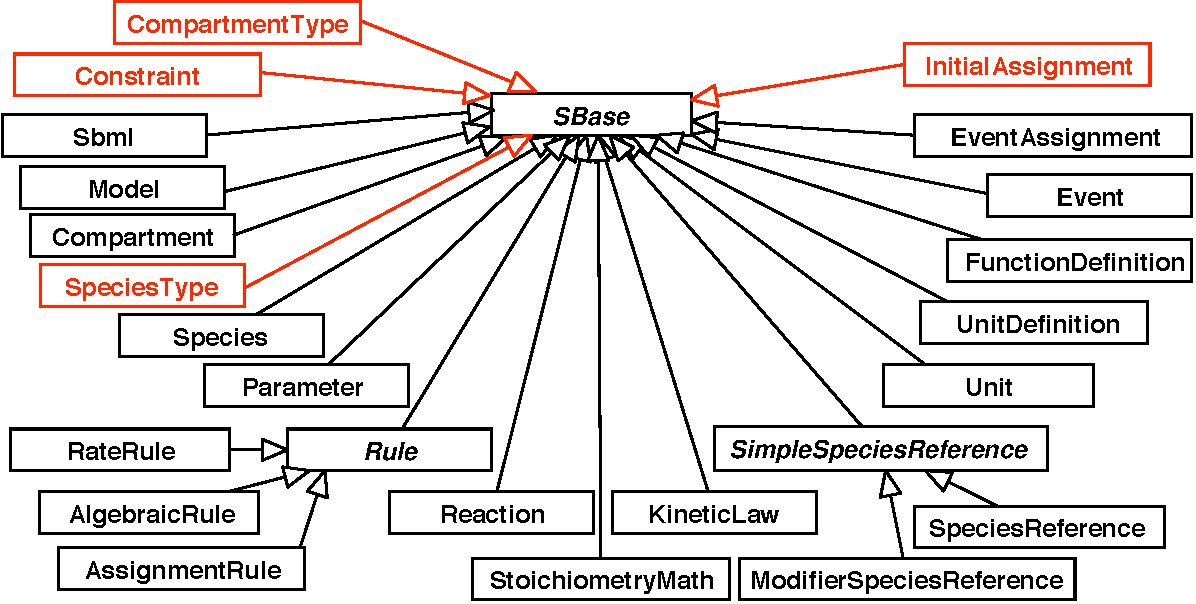
\includegraphics[scale = 0.7]{figs/top-level}
  \caption{A UML diagram of the inheritance hierarchy of major data types
    in SBML.  Open arrows indicate inheritance, pointing from inheritors to
    their parents~\protect\citep{eriksson:1998,oestereich:1999}.  In addition to
    these types, all substructures in SBML (including, for example, all the
    \token{listOf} lists) are also derived from \SBase.  See text
    for details.}
  \label{fig:top-level}
\end{figure}


%-----------------------------------------------------------------------------
\subsection{\changed{Type SBase}}
\label{sec:sbase}
%-----------------------------------------------------------------------------

Every structure composing an SBML Level~2 model definition has a
specific data type that is derived directly or indirectly from a
single abstract type called \SBase.  \changed{In addition to
serving as the parent class for most other classes of objects in
SBML, this} base type is designed to allow a modeler
or a software package to attach arbitrary information to each major
structure or list in an SBML model.  The definition of \SBase is
presented in Figure~\vref{fig:sbase}.

In addition, the \token{listOf\rule{0.5in}{0.5pt}} lists and all
substructures such as \token{trigger} on \Event
(Section~\ref{sec:events}) are also derived from \SBase.  (However,
the \token{notes} and \token{annotation} fields in
\SBase, discussed below, are not derived from \SBase.)

\begin{figure}[hbt]
  \centering
  \begin{classbox}{\textsl{SBase}}
    metaid: ID \{ use="optional" \}                                                                 \\
    notes: (ANY : \{ namespace="http://www.w3.org/1999/xhtml" \}) \{ minOccurs="0" maxOccurs="1" \} \\
    annotation: (ANY) \{ minOccurs="0" maxOccurs="1" \}                                             \\
  \end{classbox}
  \caption{The definition of \SBase.  Text enclosed in braces next
    to field types (e.g., \token{\{minOccurs="0"\}}) indicates
    constraints on the possible field values.  We use the XML Schema
    language to express constraints because we are primarily interested in
    the XML encoding of SBML.  The constraint expression
    \token{\{use="optional"\}} means that the indicated field is optional
    and may be omitted in a particular instance in a model.  The constraint
    expression \token{minOccurs="0"} likewise means the indicated
    field is optional; this alternate form of expression must be used for
    those fields that are containers (i.e., fields encoded as
    subelements in XML).}
  \label{fig:sbase}
\end{figure}

\SBase contains three fields, all of which are optional:
\token{metaid}, \token{notes} and \token{annotation}. These
fields are discussed separately in the following subsections.


\subsubsection{The \token{metaid} Field}
\label{sec:metaid}

\begin{blockChanged}
The \token{metaid} field is present for supporting metadata
annotations using RDF~\cite[Resource Description
Format;][]{lassila:1999}.  It has a data type of XML \token{ID} (the
XML identifier type), which means each \token{metaid} value must be
globally unique within an SBML file.  The \token{metaid} value serves to
identify the element so that it can be referenced by metadata
placed within \token{annotation} structures (see Section~\ref{sec:annotation-use}).  Such
metadata can use RDF \token{description} elements in
which the RDF \token{describes} attributes contain the values of
the \token{metaid}'s of objects in the SBML model.
\end{blockChanged}

%The form of the RDF element content in SBML should follow the form
%described in the CellML Metadata
%Specification~\citep{cuellar:2002}.


\subsubsection{The \token{notes} Field}

The field \token{notes} in \SBase is a container for
XHTML\changed{~1.0~\citep{pemberton:2002}} content.  It is
intended to serve as a place for storing optional information
intended to be seen by humans.  \changed{An example use of the
  \token{notes} field would be to contain formatted user comments}
about the structure in which the \token{notes} field is enclosed.
Every data object derived directly or indirectly from type \SBase
can have a separate value for \token{notes}, allowing users
considerable freedom when adding comments to their models.

\begin{blockChanged}
The content of \token{notes} must declare the use of the XHTML
namespace.  The proper namespace URI is
\uri{http://www.w3.org/1999/xhtml}.  There are multiple ways in
which this can be done.  One way is to place the namespace
declaration on the top-level \Sbml object (see
Section~\ref{sec:sbml}) and then reference the namespace in the
\token{notes} content.  The following example illustrates this
approach:

\begin{example}
<sbml xmlns="http://www.sbml.org/sbml/level2/version2" level="2" version="2"
      xmlns:xhtml="http://www.w3.org/1999/xhtml">
  ...
  <notes>
    <xhtml:body>
      <xhtml:center><xhtml:h2>A Simple Mitotic Oscillator</xhtml:h2></xhtml:center>
      <xhtml:p>A minimal cascade model for the mitotic oscillator
      involving cyclin and cdc2 kinase</xhtml:p>
    </xhtml:body>
  </notes>
  ...
\end{example}

Another approach is to declare the XHTML namespace within the
\token{notes} content itself.  The following is an example of this
approach:

\begin{example}
...
<notes>
  <body xmlns="http://www.w3.org/1999/xhtml">
    <center><h2>A Simple Mitotic Oscillator</h2></center>
    <p>A minimal cascade model for the mitotic oscillator
    involving cyclin and cdc2 kinase</p>
  </body>
</notes>
...
\end{example}

Still other approaches are possible.  Section~\ref{sec:examples}
provides additional examples of using \token{notes} in different
models.

XHTML~1.0 is simply a formulation of HTML~4 in XML~1.0.  This
means the full power of HTML formatting is available for use in
\token{notes} content.  The intention behind requiring XHTML for
\token{notes} content is to regulate the format of notes in a way
that software developers will hopefully find easy to support, yet
at the same time, to provide enough regulation on the format that
users can predict to some degree how their notes will be displayed
in different tools and environments.  Libraries for displaying and
editing HTML content are commonly available in contemporary
software programming environments, and software developers may
wish to avail themselves of these facilities rather than
implementing their own XHTML support systems.

\end{blockChanged}


\begin{blockChanged}
\subsubsection{The \token{annotation} Field}
\label{sec:annotation-use}

Whereas the \token{notes} field described above is a container for content
to be shown directly to humans, the \token{annotation} field is a
container for optional software-generated content \emph{not} meant to be
shown to humans.  Every data object derived from \SBase can have its
own value for \token{annotation}.  The field's data type is XML type
\token{any}, allowing essentially arbitrary data content.  SBML places only
a few restrictions on the organization of the content; these are intended
help software tools read and write the data as well as help reduce
conflicts between annotations added by different tools.


\paragraph{The Use of XML Namespaces in \token{annotation}}

% FIXME 2006-03-19:
% we should mention that RDF is an additional thing that can show
% up in annotations.  basically what's happening here is that we're
% saying any/all rdf content must be lumpted together in one place

At the outset, software developers should keep in mind that multiple
software tools may attempt to read and write annotation content.  To reduce
the potential for collisions between annotations written by different
applications, \sbmltwotwo stipulates that tools must use XML
namespaces~\citep{bray:1999} to specify the intended vocabulary of every
annotation.  The application's developers must choose a URI
(\emph{Universal Resource Identifier}; \citealt{harold:2001,w3c:2000})
reference that uniquely identifies the vocabulary the application will use,
and a prefix string for the annotations.  Here is an example.  Suppose an
application uses the URI \uri{http://www.mysim.org/ns} and the
prefix \token{mysim} when writing annotations related to screen layout.
The content of an annotation might look like the following:

\begin{example}
<annotation>
    <mysim:nodecolors xmlns:mysim="http://www.mysim.org/ns"
         mysim:bgcolor="green"
         mysim:fgcolor="white"/>
</annotation>
\end{example}

In this particularly simple case, the content consists of a single XML
element (\token{nodecolors}) with two attributes (\token{bgcolor},
\token{fgcolor}), all of which are prefixed by the string \token{mysim}.
(Presumably this particular content would have meaning to the hypothetical
application in question.)  The content in this particular example is small,
but it should be clear that there could easily have been an arbitrarily large
amount of data placed inside the \token{mysim:nodecolors} element.

The key point of the example above is that application-specific annotation data
is entirely contained inside a single \emph{top-level element} within the
SBML \token{annotation} container.  \sbmltwotwo places the following
restrictions on annotations:
\begin{itemize}
  
\item Within a given SBML \token{annotation} element, there can
  only be one top-level element using a given namespace.
  
\item No top-level element in an \token{annotation} may use an
  SBML XML namespace, either explicitly by referencing one of the
  SBML XML namespace URIs or implicitly by failing to specify any
  namespace on the annotation.  (As of \sbmltwotwo, the defined
  SBML namespaces are the following URIs:
  \uri{http://www.sbml.org/sbml/level1},
  \uri{http://www.sbml.org/sbml/level2}, as well as
  \uri{http://www.sbml.org/sbml/level2/version2}.)
  
\item The ordering of top-level elements within a given
  \token{annotation} element is \emph{not} significant.  An
  application should not expect that its annotation content
  appears first in the \token{annotation} element, nor in any
  other particular location.

\end{itemize}

The use of XML namespaces in this manner is intended to improve the ability
of multiple applications to place annotations on SBML model structures with
reduced risks of interference or name collisions.  Annotations stored by
different simulation packages can therefore coexist in the same model
definition.  The rules governing the content of \token{annotation} elements
are designed to enable applications to easily add, change, and remove their
annotations from SBML elements while simultaneously preserving annotations
inserted by other applications when mapping SBML from input to output.

Some more examples hopefully will make this more clear.  The next
example is invalid because it contains a top-level element in the
SBML XML namespace---this happens because no namespace is declared
for the \token{<cytoplasm>} element, which means by default it
falls into the SBML namespace:

\begin{example}
<annotation>
    <cytoplasm/>
</annotation>
\end{example}

The following example is invalid because it contains two top-level
elements using the same XML namespace.  Note that it does not
matter that these are two different top-level elements
(\token{<nodecolors>} and \token{<textcolors>}); what matters is
that these separate elements are both in the same namespace rather
than having been collected and placed inside one overall container
element for that namespace.

\begin{example}
<annotation>
    <mysim:nodecolors xmlns:mysim="http://www.mysim.org/ns"
        mysim:bgcolor="green"
        mysim:fgcolor="white"/>
    <mysim:textcolors xmlns:mysim="http://www.mysim.org/ns"
        mysim:bgcolor="green"
        mysim:fgcolor="white"/>
</annotation>
\end{example}

On the other hand, the following example is valid:

\begin{example}
<annotation>
    <mysim:geometry xmlns:mysim="http://www.mysim.org/ns"
         mysim:bgcolor="green" mysim:fgcolor="white">
        <graph:node xmlns:graph="http://www.graph.org/ns" graph:x="4" graph:y="5" />
    </mysim:geometry>
    <othersim:icon xmlns:othersim="http://www.othersim.com/">
        WS2002
    </othersim:icon>
</annotation>
\end{example}

It is worth keeping in mind that although XML namespace names must
be URI references, they are (like all XML namespace names)
\emph{not required} to be directly usable in the sense of
identifying an actual, retrieval document or resource on the
Internet~\citep{bray:1999}.  URIs such as
\uri{http://www.mysim.org/} may appear as though they are (\eg)
Internet addresses, but there are not the same thing.  This style
of URI strings, using a domain name and other parts, is only a
simple and commonly-used way of creating a unique name string.

Finally, note that the namespaces being referred to here are XML
namespaces specifically in the context of the \token{annotation}
field on \SBase.  The namespace issue here is unrelated to the
namespaces discussed in \changed{Section~\ref{sec:identifiers} in the
context of component identifiers in SBML.}


\paragraph{Content of Annotations and Implications for Software Tools}

The \token{annotation} field in the definition of \SBase
exists in order that software developers may attach optional
application-specific data to the structures in an SBML model. However,
it is important that this facility not be misused.  In particular,
it is \emph{critical} that data essential to a model definition
\changed{or that can be encoded in existing SBML
structures} is \emph{not} stored in \token{annotation}. Parameter
values, functional dependencies between model structures, etc.,
should not be recorded as annotations.  It is crucial to keep in
mind the fact that data placed in annotations can be freely ignored by
software applications.  If such data affects the interpretation
of a model, then software interoperability is greatly impeded.

Here are examples of the kinds of data that may be appropriately
stored in \token{annotation}: (a) information about the graphical
layout of model components; (b) application-specific processing
instructions that do not change the essential meaning of a model;
(c) identification information for cross-referencing components in
a model with items in a data resource such as a database.

\paragraph{Standardized Format for Certain Classes of Annotations}

For case (c) above (i.e., information for cross-referencing components in a
model to data resources), \sbmltwotwo recommends a standard format for use
within an \token{annotation} field.  This format should be used in
preference to proprietary syntaxes to maximize the likelihood that multiple
software tools will converge on the same syntax for this kind of
information.  The \sbmltwotwo recommended scheme is described in
Section~\ref{sec:finney-novere}.

\end{blockChanged}


%-----------------------------------------------------------------------------
\subsection{The \token{id} and \token{name} Fields on SBML Components}
\label{sec:idnameattribs}
%-----------------------------------------------------------------------------

\begin{blockChanged}

As will become apparent below, most structures in SBML include two
common fields: \token{id} and \token{name}.  These fields are not
defined on \SBase (as explained in
Section~\ref{sec:why-not-on-sbase} below), but where they do
appear, the common rules of usage described below apply.


\subsubsection{The \token{id} Field and Identifier Scoping}
\label{sec:identifiers}

The \token{id} field is a mandatory field on most structures in
SBML.  It is used to identify a component within the model
definition.  Other SBML structures can refer to the component
using this identifier.  Section~\ref{sec:sid} provides a
definition of the data type \primtype{SId} used for the \token{id}
field.

\end{blockChanged}

A biochemical network model can contain a large number of
components representing different parts of a model.  This leads to
a problem in deciding the scope of an identifer: in what contexts
does a given identifier \emph{X} represent the same thing?  The
approaches used in existing simulation packages tend to fall into
two categories which we may call global and local.  The
\emph{global} approach places all identifiers into a single global
namespace, so that an identifier \emph{X} represents the same
thing wherever it appears in a given model definition.  The
\emph{local} approach places symbols in different namespaces
depending on the context, where the context may be, for example,
individual reaction rate expressions.  The latter approach means
that a user may use the same identifer \emph{X} in different rate
expressions and have each instance represent a different quantity.

The fact that different simulation programs may use different
rules for identifier resolution poses a problem for the exchange
of models between simulation tools.  Without careful
consideration, a model written out in SBML format by one program
may be misinterpreted by another program.  \sbmltwo must
therefore include a specific set of rules for treating identifers
and \changed{their scopes}.

The \changed{scoping} rules in \sbmltwo are relatively straightforward
and are intended to avoid this problem with a minimum of
requirements on the implementation of software tools:
\begin{itemize}

\item \changed{The identifiers (\ie the values of the field
  \token{id}) of functions, compartment types, compartments,
  species types, species, reactions, species references,
  modifier species references, events, global parameters,
  and the model object, must be unique across the set of all
  such identifiers in the model.  This means, for example, that
  a reaction and a species definition cannot both have the same
  identifier.}

\item Each \changed{\Reaction instance} (see
  Section~\ref{sec:reactions}) establishes a private local
  namespace for local parameter identifiers.  Within the
  definition of a given reaction, local parameter identifiers
  introduced in that reaction override (shadow) identical
  identifers \changed{outside of that reaction}.  \changed{Of
    course, the corollary of this is that local parameters inside
    a \Reaction object instance are not visible to other objects
    outside of that reaction.}

\item Unit identifiers (the values of the field \token{id} in the
  \UnitDefinition structure) exist in a separate global namespace
  distinct from other identifiers.

\end{itemize}

The set of rules above can enable software packages using either
local or global namespaces for parameters to exchange SBML model
definitions.  In particular, software environments using local
namespaces for parameters internally should, in principle, be able
to accept SBML model definitions without needing to change
component identifiers.  Environments using a global namespace for
parameters internally can perform manipulations of the identifiers
of local parameter elements within reaction definitions to avoid
name collisions.

% [2006-04-01 AF] Removed the following because a its not >that< simple and
% the the approach you outline is not bullet proof and I don't
% think its a good idea to create a hostage to fortune for
% naive implementors.  In practice you have to (a) ensure the
% generated ids use a seperator (e.g. '.') that contains one or more characters
% that are not valid sbml id characters (to eliminate other namespace colisions)
% (this assumes you never write out the transformed model as SBML!!)
% (b) substitute the new ids into the kinetic law (c) add the new ids to the
% global parameter list.
%
%(An example approach for
%the latter would be the following: when receiving an SBML-encoded
%model, prefix each parameter identifier inside each reaction with
%a string constructed from the reaction's identifier; when writing
%an SBML-encoded model, strip off the prefix.)

The namespace rules described here will hopefully provide a clean
transition path to future levels of SBML, when submodels are
introduced (Section~\ref{sec:level-3}).  Submodels will provide
the ability to compose one model from a collection of other
models.  This capability will have to be built on top of \sbmltwo's
namespace organization.  A straightforward approach to
handling namespaces is to make each submodel's space be private.
The rules governing namespaces within a submodel can simply be the
Level~2 namespace rule described here, with each submodel having
its own (to itself, global) namespace.


\subsubsection{The \token{name} Field}
\label{sec:name}

In contrast to the \token{id} field, the \token{name} field is
optional and is not intended to be used for cross-referencing
purposes within a model.  Its purpose instead is to provide a
human-readable label for the component.  The data type of the
\token{name} field is the type \primtype{string} defined in XML
Schema~\citep{biron:2000,thompson:2000} and discussed further in
Section~\ref{sec:primitive-types}.  SBML imposes no restrictions
as to the content of \token{name} fields beyond those restrictions
defined by the \primtype{string} type in XML Schema.

The recommended practice for handling \token{name} is as follows.
If a software tool has the capability for displaying the content
of \token{name} fields, it should display this content to the user
as a component's label instead of the component's \token{id}
field.  If the user interface does not have this capability (e.g.,
because it cannot display or use special characters in symbol
names), or if the \token{name} field is missing on a given
component, then the user interface should display the value of the
\token{id} field instead.  (Script language interpreters are
especially likely to display \token{id} fields instead of
\token{name} fields.)

As a consequence of the above, authors of systems that
automatically generate the values of \token{id} fields should be
aware some systems may display the \token{id}'s to the user.
Authors therefore may wish to take some care to have their
software create \token{id} values that are reasonably easy for
humans to type and read.

\begin{blockChanged}
An additional point worth mentioning is although there are
restrictions on the uniqueness of \token{id} values (see
Section~\ref{sec:identifiers} below), there are no restrictions on
the uniqueness of \token{name} values in a model.  This allows
software packages leeway in assigning component identifiers.
\end{blockChanged}

%For example, a species in an SBML model must be
%located in a compartment, which means that if the same species appears in
%multiple compartments (e.g., in the context of a transport reaction), they
%must be given different identifiers.  It is currently the case that users
%and software differ sharply in philosophy about how to treat this
%situation: some treat these as different species, and others treat them as
%the same species located in different places.  Those in the latter group
%often want to use the same \token{name} but have different \token{id}
%values for the differently-localized ``instances'' of the species.  The
%freedom from restrictions on \token{name} values enables SBML to
%accommodate both philosophies.


\begin{blockChanged}

\subsubsection{Identifiers, Names, and \class{SBase}}
\label{sec:why-not-on-sbase}

% [MH 2006-03-06] Most of the following issues could be addressed
% by having a separate "SBaseWithId" class.  I think only the first
% two reasons couldn't be addressed.  Thus, the original paragraph
% (which only talked about scoping) was almost in some sense the
% fundamental reason.  I added this other stuff to address some
% questions made in the past, but these other arguments are all
% trumped by saying ``just define an SBaseWithID''.  Therefore,
% it may be worth thinking about going back to the single reason.

Although many SBML components also feature two other fields named
\token{id} and \token{name}, these fields are purposefully not defined on
\SBase.  There are several reasons for this.
\begin{itemize}

\item The identifier field is optional on some SBML components and
  required on others.  Putting \token{id} on \SBase would make it
  impossible to accommodate both cases---it would force
  identifiers to be mandatory on all components.

\item The \SBase abstract type is used as the base type for
  certain structures such as \Unit, \AssignmentRule,
  \AlgebraicRule, etc., which do not have identifiers at all
  because these structures do not need to be referenced by other
  structures.  If instead \SBase had an \token{id} field,
  all objects of these other types in a model would then need to
  be assigned unique identifiers.  This would be a needless burden
  on software developers, given that these objects do not need
  identifiers.

\item The presence of an SBML identifier field (\token{id})
  necessarily requires specifying scoping rules for the
  corresponding identifiers.  However, the \SBase abstract type is
  used as the basis for defining components whose scoping rules
  are in some cases different from each other.  (See
  Section~\ref{sec:identifiers} for more details).  If \SBase where
  to have an \token{id} field, then the specification of \SBase
  would need a default scoping rule and this would then have to be
  overloaded on derived classes that needed different scoping.
  This would make the SBML specification needlessly complex.

\item Because \SBase is the base type of the
  \token{listOf\rule{0.5in}{0.5pt}} lists (see
  Section~\ref{sec:type-inheritance-hierarchy}), putting
  \token{id} on \SBase would require all of these lists in a model
  to be given identifers.  This would again be pointless because
  these lists are only syntactic constructs; they cannot carry a
  value or be referenced by the rest of an SBML model.

\item Because the \Sbml top-level object is derived from \SBase,
  it too would have to be assigned a mandatory identifier.  Again,
  there is no functional reason to have an identifier on this
  object (it is outside the model!).  With respect to the
  \token{name} field, \SBase does not have a \token{name} simply
  because such a field is paired with an \token{id} field.

\end{itemize}

\end{blockChanged}


%-----------------------------------------------------------------------------
\subsection{Mathematical Formulas in SBML Level 2}
\label{sec:formulas}
%-----------------------------------------------------------------------------

Mathematical expressions in SBML Level~2 are represented using
\mathmltwo~\citep{w3c:2000b}, the XML standard for describing
mathematics in machine-readable format.  It is used in the
definitions of functions (Section~\ref{sec:functiondefinition}), rules
(Section~\ref{sec:rules}), initial assignments
(Section~\ref{sec:initialAssignment}), constraints
(Section~\ref{sec:constraints}), reaction kinetics
(Section~\ref{subsec:kinetic-law}), stoichiometries
(Section~\ref{subsec:speciesreference}) and events
(Section~\ref{sec:events}). The \FunctionDefinition, \KineticLaw,
\StoichiometryMath, \EventAssignment,
\changed{\InitialAssignment, \Constraint}, and
\Rule structures each have a single MathML \token{math}
subelement.  \changed{The \Event structure has two \token{math} elements, one
inside a subelement named \token{trigger} and the other inside
a subelement named \token{delay}.  The \FunctionDefinition's single
\token{math} element is limited to containing only a single MathML
\token{lambda} element.}

The XML namespace URI for all MathML elements is
\uri{http://www.w3.org/1998/Math/MathML}.  [See the W3C document by
\citet{bray:1999} for more information about using XML namespaces.]  The
examples \changed{throughout this specification} illustrate the use of this
namespace and MathML in SBML.

\changed{The semantic interpretation of MathML in the context of
SBML follows the \mathmltwo standard.  In particular, the
semantics of MathML functions follow the definitions
laid out by \cite{abramowitz:1997} and \cite{zwillinger:1988}.
Readers are directed to these sources and the MathML specification
for information about such things as which principle values of the
inverse trigonometric functions to use.}


\subsubsection{Subset of MathML Used in SBML Level 2}
\label{sec:mathmlsubset}

The subset of \mathmltwo elements used in SBML Level~2 is similar to
that used by CellML~\changed{\citep{hedley:2001b}, another model
definition language with similar goals as SBML.  The MathML
elements permitted in SBML are} itemized below:
\begin{itemize}\setlength{\parskip}{-0.2ex}

\item \emph{token}: \token{cn}, \token{ci}, \token{csymbol},
  \token{sep}

\item \emph{basic content}: \token{apply}, \token{piecewise},
  \token{piece}, \token{otherwise}

\item \emph{relational operators}: \token{eq}, \token{neq},
  \token{gt}, \token{lt}, \token{geq}, \token{leq}

\item \emph{arithmetic operators}: \token{plus}, \token{minus},
  \token{times}, \token{divide}, \token{power}, \token{root},
  \token{abs}, \token{exp}, \token{ln}, \token{log},
  \token{floor}, \token{ceiling}, \token{factorial}

\item \emph{logical operators}: \token{and}, \token{or},
  \token{xor}, \token{not}

\item \emph{qualifiers}: \token{degree}, \token{bvar},
  \token{logbase}

\item \emph{trigonometric operators}: \token{sin}, \token{cos},
  \token{tan}, \token{sec}, \token{csc}, \token{cot},
  \token{sinh}, \token{cosh}, \token{tanh}, \token{sech},
  \token{csch}, \token{coth}, \token{arcsin}, \token{arccos},
  \token{arctan}, \token{arcsec}, \token{arccsc}, \token{arccot},
  \token{arcsinh}, \token{arccosh}, \token{arctanh},
  \token{arcsech}, \token{arccsch}, \token{arccoth}

\item \emph{constants}: \token{true}, \token{false},
  \token{notanumber}, \token{pi}, \token{infinity},
  \token{exponentiale}

\item \emph{annotation}: \token{semantics}, \token{annotation},
  \token{annotation-xml}

\end{itemize}

The inclusion of logical operators, relational operators,
\token{piecewise}, \token{piece}, and \token{otherwise} elements
facilitates the encoding of discontinuous expressions.  Elements
for representing partial differential calculus are not included.
We anticipate that the requirements for partial differential
calculus will be addressed in proposals for SBML Level~3 geometry
representations (see Section~\ref{sec:level-3}).

\changed{Parsers should take particular note of the MathML
semantics of the N-ary operators \token{plus}, \token{times},
\token{and}, \token{or} and \token{xor}, when they are used
with different numbers of arguments.  The MathML
specification~\citep{w3c:2000b} appendix C.2.3 describes the
semantics for these operators with zero, one, and more arguments.}

The following are the only attributes permitted on MathML elements
in SBML:
\begin{itemize}\setlength{\parskip}{-0.2ex}

\item \token{style}, \token{class} and \token{id} on any element;

\item \token{encoding} and \token{definitionURL} on
  \token{csymbol} elements; and

\item \token{type} on \token{cn} elements.

\end{itemize}

Missing values for these attributes are to be treated in the same
way as defined by MathML.  These restrictions on attributes are
designed to confine the MathML elements to their default semantics
and to avoid conflicts in the interpretation of the type of token
elements.


\subsubsection{\changed{Handling of Whitespace}}
\label{sec:whitespace}

\begin{blockChanged}
\mathmltwo defines ``whitespace'' in the same way as XML does,
\ie the space character (Unicode hexadecimal code 0020),
horizontal tab (code 0009), newline or line feed (code 000A), and
carriage return (code 000D).  In MathML, the content of elements
such as \token{cn} and \token{ci} (described below) can be
surrounded by whitespace characters.  Prior to using the content,
this whitespace is ``trimmed'' from both ends: all whitespace at
the beginning and end of the content is
removed~\cite{ausbrooks:2003}.

For example, in a MathML element \texttt{<cn> 42 </cn>}, the amount of
white space on either side of the ``\texttt{42}'' inside the \texttt{<cn>}
\ldots\ \texttt{</cn>} container does not matter.  Prior to interpreting
the content, the whitespace is removed altogether.
\end{blockChanged}


\subsubsection{Use of \token{cn} Elements in MathML Expressions in SBML}
\label{sec:cn-token}

% FIXME put a bit more in the lead-in paragraph, such as about the
% use of type=.  The cn is not fully explained anywhere else in
% the spec.

\changed{The content of a \token{cn} element must be a number. The
number can be preceded and succeeded by whitespace.}

The following are the only permissible values for the
\token{type} attribute on MathML \token{cn} elements:
``\token{e-notation}'', ``\token{real}'',
``\token{integer}'', and ``\token{rational}''.  The
value of the \token{type} attribute defaults to
``\token{real}''.

\begin{blockChanged}
The values of the content of \token{cn} elements do not
necessarily conform to any specific floating point or integer
representations designed for CPU implementation. For example the
value of a \token{cn} element may exceed the maximum value that
can be stored in a IEEE 64 bit floating point number (IEEE 754).
This is different from the XML Schema type \primtype{double} that is
used in the definition floating point fields of structures in the
SBML namespace which \emph{is} restricted to IEEE double-precision
64-bit floating point type IEEE 754-1985.  (Integer fields in the
SBML namespace are only restricted by sign in some cases. The
absolute size of field integer values is not restricted.)

It is important to note that MathML uses a style of
scientific notation that differs from what is defined in XML Schema.
The \mathmltwo ``\token{e-notation}'' requires the mantissa and exponent to
be separated by one \texttt{<sep/>} element.  The mantissa must
be a real number and the exponent part must be a signed
integer.  This leads to expressions such as

\begin{example}
<cn type="e-notation"> 2 <sep/> -5 </cn>
\end{example}

for the number $2 \times 10^{-5}$.  It is especially
important to note that the expression

\begin{example}
<cn type="e-notation"> 2e-5 </cn>
\end{example}

is \emph{not valid} in \mathmltwo.  In the SBML XML namespace,
when an attribute value is declared to have type
\primtype{double} (a type taken from XML Schema), the
compact notation ``\texttt{2e-5}'' is in fact allowed, but not
inside the MathML XML namespace. (This is a regrettable difference
between two standards that SBML replies upon, but it is not
feasible to redefine these types within SBML because the result
would be incompatible with parser libraries written to conform
with the MathML and XML Schema standards.  It is also not possible
to use XML Schema to define a data type for SBML attribute values
permitting the use of the \token{<sep/>} notation, because XML
attribute values cannot contain XML elements: \token{<sep/>}
cannot appear in an XML attribute value.)
\end{blockChanged}


\subsubsection{Use of \token{ci} Elements in MathML Expressions in SBML}
\label{sec:ci-token}

\changed{The content of a \token{ci} element must be an SBML identifier
that is declared elsewhere in the model.  The identifier can be
preceded and succeeded by whitespace.} The set of possible
identifiers that can appear in a \token{ci} element depends on the
containing structure in which the \token{ci} is used:
\begin{itemize}

\item If a \token{ci} element appears in the body of a function definition
  \changed{(Section~\ref{sec:functiondefinition})}, the
  referenced identifier must be either (i) one of the declared arguments to
  that function, or (ii) the identifier of a previously defined function.

\item \changed{In all other situations, the referenced identifier must be the
  identifier of a species, compartment, parameter, function or reaction declared in
  the model.}  The following are the only possible interpretations of using
  such an identifier in SBML:
  \begin{itemize}

  \item \emph{Species identifier}: When a species identifier occurs in a
    \token{ci} element, it represents the quantity (\quantity{amount of substance}
    or \quantity{concentration}) of that species.
    The units associated with a species identifier are
    \emph{the units of the species}, defined in
    Section~\ref{sec:species-units}.

  \item \emph{Compartment identifier}: When a compartment identifier occurs
    in a \token{ci} element, it represents the size of the compartment.
    The units associated with the size of the compartment are those
    given on the \Compartment structure that declares the identifier;
    see Section~\ref{sec:compartment-units}.

  \item \emph{Parameter identifier}: When a parameter identifier occurs in
    a \token{ci} element, it represents the \changed{numerical} value assigned to that
    parameter.  The units associated with the parameter value are the units
    assigned in its instance of a \Parameter structure; see
    Section~\ref{sec:parameter-units}.

  \item \emph{Function identifier}: When a function identifier occurs in a
    \token{ci} element, it represents a call to that function.  Function
    references in MathML occur in the context of using MathML's
    \token{apply} and often involve supplying arguments to the function;
    see Section~\ref{sec:functiondefinition}.

  \item \changed{\emph{Reaction identifier}: When a reaction
    identifier occurs in a \token{ci} element, it represents the
    rate of the reaction, which is given by the kinetic law of the
    reaction if present.  The units associated with the reaction
    value are the units assigned to the \KineticLaw structure
    contained within the \Reaction structure; see
    Section~\ref{subsec:kinetic-law}.  (The units of the reaction
    identifier follow the defaults described in
    Section~\ref{subsec:kinetic-law} when the \KineticLaw
    structure is not present.)}

  \end{itemize}

\end{itemize}

\changed{The content of \token{ci} elements outside a
\KineticLaw and \FunctionDefinition structures
always refer to objects declared in the top level global namespace;
i.e., SBML uses ``early binding'' semantics.  The only \token{ci}
elements that can represent parameters listed in a
\KineticLaw structure are those \token{ci} elements
contained in the \KineticLaw structure (see
Section~\ref{subsec:kinetic-law}).}


\subsubsection{Use of \token{csymbol} Elements in MathML Expressions in SBML}
\label{sec:csymbol-token}

SBML Level 2 uses the MathML \token{csymbol} element to denote certain
built-in mathematical entities without introducing reserved names into the
component identifier namespace.  The \token{encoding} field of
\token{csymbol} should be set to ``\token{text}''.  The
\token{definitionURL} should be set to one of the following predefined
SBML symbol URIs:
\begin{itemize}

\item \uri{http://www.sbml.org/sbml/symbols/time}.  This represents the
  current simulation time.  The units of the current time entity are
  determined from the built-in \token{time} of Table~\vref{tab:builtin}.

\item \uri{http://www.sbml.org/sbml/symbols/delay}.  This represents a delay
  function.  The delay function has the form $delay(x, d)$, taking two
  \changed{MathML expressions as} arguments.  Its value is the value of argument
  $x$ at $d$ time units before the current time.  \changed{There are no
  restrictions on the form of $x$.} The units of the $d$ parameter
  are determined from the built-in \token{time}.  \changed{The value of the $d$
  parameter, when evaluated, must be numerical and be greater than or equal to 0.}
  The \texttt{delay} function is useful
  for representing biological processes having a delayed response, but
  where the detail of the processes and delay mechanism is not relevant to
  the operation of a given model.

\end{itemize}

The following examples demonstrate these concepts.  The XML fragment below
encodes the formula $x + t$, where $t$ stands for time.
\begin{example}
<math xmlns="http://www.w3.org/1998/Math/MathML">
    <apply>
        <plus/>
        <ci> x </ci>
        <csymbol encoding="text" definitionURL="http://www.sbml.org/sbml/symbols/time">
            t
        </csymbol>
    </apply>
</math>
\end{example}

\begin{blockChanged}
In the fragment above, the use of the token \texttt{t} is mostly a
convenience for human readers---the string inside the \texttt{csymbol} could
have been almost anything, because it is essentially ignored by MathML
parsers and SBML.  Some MathML and SBML processors will take note of the
token and use it when presenting the mathematical formula to users, but the
token used has no impact on the interpretation of the model and it does not
enter into the SBML component identifier namespace.  In other words, the
content of the \token{csymbol} element is for rendering purposes only and
can be ignored by the parser.
\end{blockChanged}

As a further example, the following XML fragment encodes the equation
$k + delay(x, 0.1)$ or alternatively $k_t + x_{t - 0.1}$:
\begin{example}
<math xmlns="http://www.w3.org/1998/Math/MathML">
    <apply>
        <plus/>
        <ci> k </ci>
        <apply>
            <csymbol encoding="text" definitionURL="http://www.sbml.org/sbml/symbols/delay">
                delay
            </csymbol>
            <ci> x </ci>
            <cn> 0.1 </cn>
        </apply>
    </apply>
</math>
\end{example}

Note that the URI in the value of ``\token{definitionURL}'', as all
URIs, are intended to serve as unique identifiers and are not intended to
be dereferenced as Internet addresses.

\begin{blockChanged}

\subsubsection{Math Expression Types}
\label{sec:mathmltype}

MathML operators in SBML each return results in one of two possible types:
boolean and numeric.  The following guidelines summarize the different
possible cases.

The relational operators (\token{eq}, \token{neq},
\token{gt}, \token{lt}, \token{geq}, \token{leq}), the logical
operators (\token{and}, \token{or}, \token{xor}, \token{not}), and
the boolean constants (\token{false}, \token{true}) always return
boolean values.

The type of an operator referring to an SBML \FunctionDefinition is
determined by the type of the top-level operator of the MathML expression
in the \token{math} field of the function definition.  This type may be
boolean or numeric.

All other operators, values and symbols return numeric results.

The roots of the expression trees used in the following contexts
must yield boolean values:
\begin{itemize}

\item the arguments of the MathML logical operators (\token{and},
\token{or}, \token{xor}, \token{not});

\item the second argument of a MathML \token{piece} operator;

\item the \token{trigger} field of an SBML \Event structure; and

\item the \token{math} field of an SBML \Constraint structure.

\end{itemize}

The roots of the expression trees used in the following contexts can
optionally yield boolean values:
\begin{itemize}

\item the arguments to the \token{eq} and \token{neq} operators;

\item the first arguments of MathML \token{piece} and \token{otherwise}
operators; and

\item the top level expression of a function definition.

\end{itemize}

The roots of expression trees in other contexts must yield numeric
values.

The type of expressions should be used consistently.  The set of
expressions that make up the first arguments of the \token{piece}
and \token{otherwise} operators within the same \token{piecewise}
operator should all return values of the same type. The arguments
of the \token{eq} and \token{neq} operators should return the same
type.

\end{blockChanged}

%\subsubsection{N-ary Operators}
%\label{sec:nary-operators}
%
%The use of N-ary operators (\token{add}, \token{times}, \token{and},
%\token{or} and \token{xor}) should follow their definition in the MathML
%specification.  However, the MathML specification does not define the
%semantics of the operators with zero or one operand.  Here we define the
%relevant semantics for SBML.  The general form of the operators is
%
%\begin{center}
%f($x_1$ ... $x_n$) = base\_operand operator $x_1$ operator \ldots\ $x_n$
%\end{center}
%
%where $n$ is any non-negative integer and base\_operand is a
%constant that is associated with the operator.  The base\_operand
%can be considered an additional hidden operand to the operator.
%Table~\ref{tab:baseoperands} gives the base operands for the N-ary
%operators of the MathML subset used in SBML.
%
%\begin{table}[bh]
%  \begin{blockChanged}
%  \small
%  \centering
%  \begin{tabular}{ll}
%    \toprule
%    Operator & Base Operand \\
%    \midrule
%    \token{add} & 0 \\
%    \token{times} & 1 \\
%    \token{and} & true \\
%    \token{or} & false \\
%    \token{xor} & false \\
%    \bottomrule
%  \end{tabular}
%  \vspace*{-0.95ex}
%  \caption{The base operands of the N-ary operators of the MathML subset in
%    SBML.}
%  \label{tab:baseoperands}
%  \end{blockChanged}
%\end{table}
%
%For example
%
%\begin{example}
%<apply>
%    <add/>
%<apply/>
%\end{example}
%
%returns $0 = 0$;
%
%\begin{example}
%<apply>
%    <add/>
%    <cn>7</cn>
%<apply/>
%\end{example}
%
%returns $7 = 0 + 7$; and
%
%\begin{example}
%<apply>
%    <add/>
%    <cn>7<cn/>
%    <cn>13<cn/>
%</apply>
%\end{example}
%
%returns $20 = 0 + 17 + 13$.
%
%Numerical computations involving the N-ary operators can be
%optimized by performing replacements on the operators when certain
%conditions apply.  Specifically, the operator can be replaced by
%the base\_operand if the operator has no operands; or by an
%operand if the operator has only one operand (i.e.,  the operator
%is equivalent to identity).
%\end{blockChanged}

%=============================================================================
\section{SBML Components}
\label{sec:elements}
%=============================================================================

In this section, we define each of the major data structures in SBML. To
provide illustrations of their use, we give partial model definitions in
XML.  Section~\ref{sec:xml-rep} provides many full examples of SBML in XML.

\begin{blockChanged}
In type definitions presented throughout this section section, we follow the UML
convention of hiding the attributes derived from a parent type such as
\SBase. It should be kept in mind that these attributes are always
available.
\end{blockChanged}


%-----------------------------------------------------------------------------
\subsection{The SBML Container}
\label{sec:sbml}
%-----------------------------------------------------------------------------

The outermost portion of an SBML Level~2 model definition consists of a
single \Sbml structure enclosing a single \Model structure
(see next Section).  The definition of \Sbml is shown in
Figure~\ref{fig:sbml}.

\begin{figure}[htb]
  \centering
  \begin{classbox}{Sbml}
    level: positiveInteger \{ use="required" fixed="2" \}             \\
    version: positiveInteger \{ use="required" fixed="\markChanged{2}" \} \\
  \end{classbox}
  \caption{The definition of \Sbml for SBML Level~2
    \changed{Version~2}.  Following UML notation, additional
    fields that are inherited from a base class, in this case
    \SBase, are not shown.}
  \label{fig:sbml}
\end{figure}

\changed{The XML namespace URI for \sbmltwotwo is
\uri{http://www.sbml.org/sbml/level2/version2}}.  All SBML
Level~2 Version~2 elements should be encoded using this URI by
assigning \changed{it} to either the default \changed{XML} namespace or a tag
prefix.  The character encoding for SBML is UTF-8.  SBML documents
should include the \token{encoding} attribute with the value
\token{UTF-8} in the XML prologue.

In the transformation of UML to XML used in this document, the \Sbml
structure is turned into an element named \texttt{sbml}.  The element has
two required attributes: \token{level} and \token{version}.  \changed{For SBML
Level~2 Version~2, these attributes must be set to ``\texttt{2}'' and
``\texttt{2}'', respectively.}

The following is an abbreviated example of the outermost content of an SBML
model definition in XML:

\begin{blockChanged}
\begin{example}
<?xml version="1.0" encoding="UTF-8"?>
<sbml xmlns="http://www.sbml.org/sbml/level2/version2" level="2" version="2">
  ...
</sbml>
\end{example}
\end{blockChanged}

\begin{blockChanged}
Readers may wonder why the SBML top-level XML element uses both a namespace
URI identifying the SBML level and version, as well as separate XML
attributes encoding the level and version.  Why is the information
duplicated?  There are several reasons.  First, XML is only one
possible serialization of SBML (albeit an extremely popular one at this
time).  Though most of this document is written with XML in mind, it is the
intention behind the design of SBML that its object structure should be
implementable in other languages and software systems.
Programmatic access is easier if the level and version information
are accessible directly as data rather than have to be extracted
from a string.  Second, generic high-level XML
parsers may give their calling programs access to the value of the \texttt{xmlns}
attribute.  Providing the information via separate attributes is a good
backup measure.  And finally, earlier in the history of SBML, it was
expected that only the level needed to be encoded as part of the namespace
URI (e.g., \uri{http://www.sbml.org/sbml/level1}) because it was
hoped that changes within levels would not require XML Schema changes.
This has proven to be false, but SBML Level~1 (both versions) and the
first version of SBML Level~2 still subscribe to this principle.  This
means that for these variants of SBML, software tools must look for a
\token{version} attribute on the top-level element.  For backwards
compatibility with software that expects this, it makes more sense to keep
the version and level attributes.
\end{blockChanged}


%-----------------------------------------------------------------------------
\subsection{Models}
\label{sec:model}
%-----------------------------------------------------------------------------

The \Model structure is the highest-level construct in an SBML data
stream or document.  Its definition is shown in
Figure~\vref{fig:model}.  Only one component of type \Model is
allowed per instance of an \changed{\sbmltwotwo} document or data stream, although it does
not necessarily need to represent a single biological entity.

\begin{figure}[htb]
  \centering
  \begin{classbox}{Model}
    id: SId  \{ use="optional" \}                        \\
    name: string \{ use="optional" \}                    \\
    \markChanged{sboTerm: SBOTerm \{ use="optional" \}}      \\
    functionDefinition: FunctionDefinition[0..*]         \\
    unitDefinition: UnitDefinition[0..*]                 \\
    \markChanged{compartmentType: CompartmentType[0..*]}     \\
    \markChanged{speciesType: SpeciesType[0..*]}             \\
    compartment: Compartment[0..*]                       \\
    species: Species[0..*]                               \\
    parameter: Parameter[0..*]                           \\
    \markChanged{initialAssignment: InitialAssignment[0..*]} \\
    rule: Rule[0..*]                                     \\
    \markChanged{constraint: Constraint[0..*]}               \\
    reaction: Reaction[0..*]                             \\
    event: Event[0..*]                                   \\
  \end{classbox}
  \caption{The definition of \Model.  Following UML notation, additional fields
    that are inherited from a base class, in this case \SBase, are not shown.}
  \label{fig:model}
\end{figure}

\changed{\Model serves as a container for components of object classes
\FunctionDefinition, \UnitDefinition,
\CompartmentType, \SpeciesType, \Compartment,
\Species,
\Parameter, \InitialAssignment,
\Rule, \Constraint, \Reaction and
\Event.} All of these components are optional;
that is, the lists in each of the respective fields are permitted
to have zero length. (However, there are dependencies between
components, such that defining some requires defining others.  For
example, as explained in other sections below, defining a species
requires defining a compartment, and defining a reaction requires
defining a species.)

The \Model structure has an optional field, \token{id}, used to
give the model an identifier.  The identifier must be a text string
conforming to the syntax permitted by the \primtype{SId} data type described
in Section~\ref{sec:sid}.  \Model also has an optional \token{name}
field, of type \primtype{string}.  The \token{name} and \token{id} fields
\changed{must} be used as described in Section~\ref{sec:idnameattribs}.

\changed{In the XML encoding of an SBML model, the lists of
compartment types, compartments, species types, species, unit
definitions, parameters, initial assignments, reactions, function
definitions, constraints, rules and events are translated into
lists of XML elements enclosed within elements of the form
\token{listOf}\rule{0.5in}{0.5pt}\token{s}, where the blank is
replaced by the name of the component type.  If the word already
ends in ``s'', such as ``species'', then the extra letter is
omitted from the end, leading to \token{listOfSpecies}.}  The
resulting XML data object has the form illustrated by the
following skeletal model:
\begin{blockChanged}
\begin{example}
<model id="My_Model">
    <listOfFunctionDefinitions>
        ...
    </listOfFunctionDefintions>
    <listOfUnitDefinitions>
        ...
    </listOfUnitDefinitions>
    <listOfCompartmentTypes>
        ...
    </listOfCompartmentTypes>
    <listOfSpeciesTypes>
        ...
    </listOfSpeciesTypes>
    <listOfCompartments>
        ...
    </listOfCompartments>
    <listOfSpecies>
        ...
    </listOfSpecies>
    <listOfParameters>
        ...
    </listOfParameters>
    <listOfInitialAssignments>
        ...
    </listOfInitialAssignments>
    <listOfRules>
        ...
    </listOfRules>
    <listOfConstraints>
        ...
    </listOfConstraints>
    <listOfReactions>
        ...
    </listOfReactions>
    <listOfEvents>
        ...
    </listOfEvents>
</model>
\end{example}
\end{blockChanged}

Readers may wonder about the motivations for the
\token{listOf}\rule{0.5in}{0.5pt}\token{s} notation.  A simpler
approach to creating the lists of components would be to place
them all directly at the top level under \texttt{<model> ...
</model>}.  We chose instead to group them within XML elements
named after \token{listOf}\rule{0.5in}{0.5pt}\token{s}, because we
believe this helps organize the components and makes visual
reading of model definitions easier.  These
\token{listOf}\rule{0.5in}{0.5pt}\token{s} elements are derived
from \SBase which enables each list to contain its own
\token{metaid}, \token{notes} and \token{annotation}
 fields. Further details of how
\token{listOf}\rule{0.5in}{0.5pt}\token{s} elements implement UML
lists is described in Section~\ref{sec:notation}.


\begin{blockChanged}
\subsubsection{The \token{sboTerm} Field}
\label{sec:model-sboterm}

The \Model structure has an optional \token{sboTerm} field of type
\primtype{SBOTerm} (see Sections~\ref{sec:sboterm-type}
and~\ref{sec:sboTerm}).  When a value is given to this field in a
model, the value must be an SBO (\sboref) identifier referring to
a modeling framework defined in SBO (\ie terms derived from
\sboframework).  The SBO term chosen should be the most precise
(narrow) term that defines the mathematical framework assumed by
the \emph{entire} model.  An example framework might be ``discrete
stochastic'', which would mean the \emph{entire} model was created
under the assumption it will be simulated in a tool that turns
substance quantities into discrete numbers and applies a
stochastic stimulation algorithm~\cite[e.g.,][]{gillespie:1977} to
the model.  Other frameworks are possible.

The value given to \token{sboTerm} on a \Model interacts with the
SBO labels on the model's \Reaction elements in the following way.
The label on \Model should apply to the model as a whole, meaning
that \emph{all} reactions in the model assume the same framework.
In that case, the \token{sboTerm} values on individual \Reaction
elements may be omitted, but only the \Reaction SBO labels can be
thus omitted; the SBO labels on \KineticLaw within \Reaction must
still be supplied, as must the terms on other components of the
model, in order to characterize the model completely.

The absence of a \token{sboTerm} value means that either the model
has not been labeled with SBO terms at all, or there was no
available SBO modeling framework term at the time the model was
created that was deemed suitable for characterizing the model as a
whole.  If \Model has no value for \token{sboTerm}, the
\token{sboTerm} fields on each \Reaction in a model may still
indicate the framework assumed for each reaction separately.

As discussed in Section~\ref{sec:sboTerm}, SBO labels are optional
information on a model.  Applications are free to ignore
\token{sboTerm} values, and a model must be interpretable without the
benefit of SBO labels.

\end{blockChanged}


%-----------------------------------------------------------------------------
\subsection{Function Definitions}
\label{sec:functiondefinition}
%-----------------------------------------------------------------------------

The \FunctionDefinition structure associates an identifier with a
function definition.  This identifier can then be used as
\changed{the function called in subsequent MathML} \token{apply}
elements.  \FunctionDefinition is shown in
Figure~\ref{fig:mathdefinition}.

\begin{figure}[htb]
  \centering
  \begin{classbox}{FunctionDefinition}
    id: SId                                                                    \\
    name: string \{ use="optional" \}                                          \\
    math: (lambda:Lambda) \{ namespace="http://www.w3.org/1998/Math/MathML" \} \\
  \end{classbox}
  \caption{The definition of \FunctionDefinition.  Following UML notation,
    additional fields
    that are inherited from a base class, in this case \SBase, are not shown.}
  \label{fig:mathdefinition}
  \label{fig:functionDefinition}
\end{figure}

\begin{blockChanged}
Function definitions in SBML (also informally known as
``user-defined functions'') have relatively limited capabilities.
As is made more clear below, a function cannot reference
parameters or other model quantities outside of itself; values
must be passed as parameters to the function.  Moreover, recursive
and mutually-recursive functions are not permitted.  The purpose
of these limitations is to balance power against complexity of
implementation.  With the restrictions as they are, function
definitions could be implemented as textual substitutions---they
are simply macros.  Software implementations may therefore not
need the full function-definition machinery typically associated
with programming languages.
\end{blockChanged}

The \FunctionDefinition structure has three fields: \token{id},
\token{name} and \token{math}.  Their purposes are explained in the
following subsections.


\subsubsection{The \token{id} and \token{name} Fields}

The \token{id} and \token{name} fields have types \primtype{SId}
and \primtype{string}, respectively, and operate in the manner
described in Section~\ref{sec:idnameattribs}.  \changed{MathML
\token{ci} elements in an SBML model can refer to the
function defined by a \FunctionDefinition using the value of its
\token{id} field.}


\subsubsection{The \token{math} Field}
\label{sec:function-definition-math}

% FIXME improve text, eg by explaining other reasons why lambdas
% can't refer to other lambdas.

The \token{math} field is a container for MathML content that
defines the function.  The content of this field can only be a
MathML \token{lambda} element.  The \token{lambda} element must
begin with zero or more \token{bvar} elements, followed by any
other of the elements in the MathML subset listed in
Section~\ref{sec:mathmlsubset} \emph{except} \token{lambda}
(\ie a \token{lambda} element cannot contain another
\token{lambda} element).  This is the only place in SBML where a
\token{lambda} element can be used.  \changed{The function defined
by a \FunctionDefinition is only available for use in other MathML
elements that \emph{follow} the \FunctionDefinition definition in
the model.  (These restrictions prevent recursive and
mutually-recursive functions from being expressed.)}

\begin{blockChanged}
A further restriction on the content of the \token{math} field is
that it cannot contain references to variables other than the
variables declared to the \token{lambda} itself.  That is, the
contents of MathML \token{ci} elements inside the body of the
\token{lambda} can only be the variables declared by its
\token{bvar} elements, or the identifiers of other
\FunctionDefinition{}s defined earlier in the model.  This implies
that functions must be written so that all variables or parameters
they may need are passed to them via their function parameters.
\end{blockChanged}


\begin{blockChanged}
\subsubsection{Examples}

The following abbreviated SBML example shows a \FunctionDefinition
structure defining \token{pow3} as the name of a function
computing the mathematical expression $x^{3}$, and after that, the
invocation of that function in the mathematical formula of a rate
law.  Note how the invocation of the function uses its identifier
\begin{example}
<model>
    ...
    <functionDefinition id="pow3">
        <math xmlns="http://www.w3.org/1998/Math/MathML">
            <lambda>
                <bvar><ci> x </ci></bvar>
                <apply>
                    <power/>
                    <ci> x </ci>
                    <cn> 3 </cn>
                </apply>
            </lambda>
        </math>
    </functionDefinition>
    ...
    <listOfReactions>
        <reaction id="reaction_1">
            ...
            <kineticLaw>
                <math xmlns="http://www.w3.org/1998/Math/MathML">
                    <apply>
                        <ci> pow3 </ci>
                        <ci> S1 </ci>
                     </apply>
                </math>
            </kineticLaw>
            ...
        </reaction>
    </listOfReactions>
    ...
</model>
\end{example}
\end{blockChanged}


%-----------------------------------------------------------------------------
\subsection{Unit Definitions}
\label{sec:unitdefinitions}
%-----------------------------------------------------------------------------

\begin{blockChanged}

Units of measurement may be supplied in a number of contexts in an
SBML model.  The units of the following mathematical entities can
be specified explicitly: the size of a compartment, the initial
amount of a species, the units of constant and variable parameter
values, the units of time and of substance in which a reaction
rate is expressed, the units of time in an event's execution
delay, and the results of mathematical formulas.  Rather than
requiring a complete unit definition on every structure, SBML
provides a facility for defining named units that can be
referenced throughout a model.  In addition, every kind of SBML
mathematical entity has units assigned to it from a set of
built-in defaults (see Section~\ref{sec:built-in-units} below, and
also Sections~\ref{sec:compartment-units}, \ref{sec:species-units}
and~\ref{subsec:kinetic-law}).  By redefining these built-in
default units, it is possible to change the units used throughout
a model in a simple and consistent manner.

The SBML unit definition facility uses two classes of objects,
\UnitDefinition and \Unit.  Their definitions are shown in
Figure~\vref{fig:unitdefinition} and explained in more detail in
Sections~\ref{sec:unitdefinition-structure}
and~\ref{sec:unit-structure} below.

\begin{figure}[htb]
  \centering
  \begin{classbox}{UnitDefinition}
    id: SId                           \\
    name: string \{ use="optional" \} \\
    unit: Unit[1..*]                  \\
  \end{classbox}
  \hspace*{2em}
  \begin{blockMarkChanged}
  \begin{classbox}{Unit}
    kind: UnitKind                                      \\
    exponent: integer \{ use="optional" default="1" \}  \\
    scale: integer \{ use="optional" default="0" \}     \\
    multiplier: double \{ use="optional" default="1" \} \\
  \end{classbox}
  \end{blockMarkChanged}
  \caption{The definition of \UnitDefinition and \Unit. Following UML
    notation, additional fields
    that are inherited from a base class, in this case \SBase, are not shown.}
  \label{fig:unitdefinition}
\end{figure}

The approach to defining units in SBML is compositional; for
example, $meter\ second^{\,-2}$ is constructed by combining a
\Unit object representing $meter$ with another \Unit object
representing $second^{\,-2}$.  The combination is wrapped inside a
\UnitDefinition, which provides for assigning an identifier and
optional name to the combination.  The identifier can then be
referenced from elsewhere in a model.

The vast majority of modeling situations requiring new SBML unit
definitions involve simple multiplicative combinations of base
units and factors.  An example of this might be ``moles per litre
per second''.  What distinguishes these sorts of simpler unit
definitions from more complex ones is that they may be expressed
without the use of an additive offset from a zero point.  The use
of offsets complicates all unit definition system, yet in the
domain of SBML the real-life cases requiring offsets are few (and
in fact, to the best of our knowledge, only involve temperature).
Consequently, the SBML unit system has been consciously designed
in a way that attempts to simplify implementation of unit support
for the most common cases in systems biology, at the cost of an
asymmetry in unit calculations introduced when offsets are used.


\subsubsection{The \class{UnitDefinition} Structure}
\label{sec:unitdefinition-structure}

A unit definition in SBML consists of an instance of a
\UnitDefinition object, shown in Figure~\ref{fig:unitdefinition}.


\paragraph{The \token{id} and \token{name} Fields}

The \token{id} and \token{name} fields have types \primtype{SId}
and \primtype{string}, respectively, and operate in the manner
summarized in Section~\ref{sec:idnameattribs}.  There are three
crucial differences between unit identifiers and most other
identifiers in SBML:
\begin{enumerate}

\item The \token{id} of a \Unit definition must not contain a
  value from Table~\ref{tab:unitkind} (\ie the enumeration of
  predefined \primtype{UnitKind} values).  This constraint simply
  prevents the redefinition of the base units.

\item Unit identifiers defined by the \token{id} field reside in a
  separate global namespace distinct from the namespace of other
  identifiers in a model; thus, unit identifiers cannot collide
  with the identifiers of species, compartments, reactions, etc.

\item There is a set of predefined identifiers for the built-in
  default units in SBML; these identifiers are \val{substance},
  \val{volume}, \val{area}, \val{length}, and \val{time}.  Using
  one of these values for \token{id} in a \UnitDefinition has the
  effect of redefining the model-wide default units for the
  corresponding quantities.  We discuss this in more detail in
  Section~\ref{sec:built-in-units}.

\end{enumerate}


\paragraph{The List of \class{Unit}s}

A \UnitDefinition object must contain one or more \Unit objects
within the \token{unit} container.  In the XML form of SBML, this
container becomes a \token{listOfUnits} element.
Section~\ref{sec:unit-structure} explains the meaning and use of
\Unit.


\paragraph{Example}

The following skeleton of a unit definition illustrates an example
use of \UnitDefinition:

\begin{example}
<listOfUnitDefinitions>
    <unitDefinition id="unit1">
        ...
    </unitDefinition>
    <unitDefinition id="unit2">
        ...
    </unitDefinition>
</listOfUnitDefinitions>
\end{example}


\subsubsection{The \class{Unit} Structure}
\label{sec:unit-structure}

A \Unit structure represents a (possibly transformed) reference to
a base unit chosen from \primtype{UnitKind}
(Table~\ref{tab:unitkind}).  The field \token{kind} indicates the
chosen base unit, whereas the three fields \token{exponent},
\token{scale}, and \token{multiplier} define how the base unit is
being transformed.  These various fields are described in detail
below.

Compatibility note: in \sbmltwoone, \Unit had an
additional field called \token{offset}.  This field has been
removed entirely from \sbmltwotwo.  Modelers and software authors
are instead directed to use other methods of encoding units
requiring offsets.  The reasons for this change, and some
suggestions for how to achieve equivalent effects of unit offsets,
are discussed in more detail below.


\paragraph{The \token{kind} Field}

\end{blockChanged}

The \Unit data structure has one required field, \token{kind},
whose value must be taken from \primtype{UnitKind}, an enumeration
of base units.  The possible values of \primtype{UnitKind} are
given in Table~\vref{tab:unitkind}.

\begin{table}[bht]
  \vspace*{1ex}
  \centering
  \ttfamily
  \small
  \setlength{\arraycolsep}{8pt}
  \begin{tabular}{llllll}
    \toprule
    ampere      & farad & joule     & lux       & radian   & volt   \\
    becquerel   & gram  & katal     & metre     & second   & watt\\
    candela     & gray  & kelvin    & mole      & siemens  & weber\\
    Celsius     & henry & kilogram  & newton    & sievert\\
    coulomb     & hertz & litre     & ohm       & steradian\\
    \underline{dimensionless} & \underline{item} & lumen     & pascal    & tesla\\
    \bottomrule
  \end{tabular}
  \caption{The possible values of \token{kind} in a \primtype{UnitKind}
    structure.  All are names of base or derived SI
    units~\protect\citep{bipm:2000}, except for
    ``\token{dimensionless}'' and ``\token{item}'', which are
    SBML additions important for handling certain common situations.
    ``\token{Dimensionless}'' is intended for cases where a quantity does not
    have units, and ``\token{item}'' for expressing
    such things as ``N items'' (e.g., ``100 molecules'').
    Also, note that the gram and litre are not
    strictly part of SI; however, they are so
    commonly used in SBML's areas of application that they
    are included as predefined unit names.  (The standard SI unit of
    mass is in fact the kilogram, and volume is
    defined in terms of cubic metres.)}
  \label{tab:unitkind}
\end{table}

Note that the set of acceptable values for the field \token{kind}
does \emph{not} include units defined by \UnitDefinition
structures.  This means that the units definition \changed{system}
in SBML is not hierarchial: user-defined units cannot be built on
top of other user-defined units, only on top of base units.  SBML
differs from CellML~\changed{\cite{hedley:2001b}} in this respect;
CellML allows the construction of hierarchial unit definitions.


\begin{blockChanged}

\paragraph{The \token{exponent}, \token{scale} and \token{multiplier} Fields}

The optional \token{exponent} field on \Unit represents an
exponent on the unit.  Its default value is \val{1} (one).  A
\Unit structure also has an optional \token{scale} field; its
value must be an integer exponent for a power-of-ten multiplier
used to set the scale of the unit.  For example, a unit having a
\token{kind} value of \val{gram} and a \token{scale} value of
\val{-3} signifies $10^{-3} * gram$, or milligrams.  The default
value of \token{scale} is \val{0} (zero), because $10^0 = 1$.
Lastly, the optional \token{multiplier} field can be used to
multiply the \token{kind} unit by a real-numbered factor; this
enables the definition of units that are not power-of-ten
multiples of SI units.  For instance, a \token{multiplier} of
0.3048 could be used to define \val{foot} as a measure of length
in terms of a metre.  The \token{multiplier} field has a default
value of \val{1} (one).

%In the following explanation of the use of these fields, we
%temporarily limit discussion to the case where offsets are not
%required (\ie when \token{offset} in a \Unit definition is not
%set, or is set to \val{0}).  We discuss the topic of offsets
%further below.

\newcommand{\ynew}{\ensuremath{y}\xspace}
\newcommand{\ybase}{\ensuremath{y_b}\xspace}
\newcommand{\unew}{\ensuremath{\{u\}}\xspace}
\newcommand{\ubase}{\ensuremath{\{u_b\}}\xspace}

The unit system allows model quantities to be expressed in units
other than the base units of Table~\ref{tab:unitkind}.  For
analyses and computations, the consumer of the model (be it a
software tool or a human) will want to convert all model
quantities to base SI units for purposes such as verifying the
consistency of units throughout the model.  Suppose we begin with
a quantity having numerical value \ynew when expressed in units
\unew.  The relationship between \ynew and a quantity \ybase
expressed in base units \ubase is
\begin{linenomath}
\begin{equation}
  \ybase \, \ubase = \ynew \, \unew \left( \frac{w \, \ubase}{\unew} \right)
\label{eq:new-to-old}
\end{equation}
\end{linenomath}
The term in the parentheses on the right-hand side is a factor for
converting a quantity in units \unew to another quantity in units
\ubase.  The ratio of units leads to canceling of \unew in the
equation above and leaves a quantity in units \ubase.  It remains
to define this factor.  In terms of the SBML unit system, it is:
\begin{linenomath}
\begin{equation}
  \unew = (\token{multiplier} \cdot 10^\token{scale} \, \ubase)^\token{exponent}
\label{eq:single-unit}
\end{equation}
\end{linenomath}
where the dot ($\cdot$) represents simple scalar multiplication.
The variables \token{multiplier}, \token{scale}, and
\token{exponent} in the equation above correspond to the fields
with the same names in the \Unit structure defined in
Figure~\ref{fig:unitdefinition}.  The exponent in the equation
above may make it more difficult to grasp the relationship
immediately; so let us suppose for the moment that
\token{exponent}=\val{1}.  Then, it is easy to see that
\begin{linenomath}
\begin{equation*}
  \unew = \token{multiplier} \cdot 10^\token{scale} \, \ubase
\end{equation*}
\end{linenomath}
Dividing both sides by \unew produces the ratio in the
parenthesized portion of Equation~\ref{eq:new-to-old}, which means
that $w = \token{multiplier} \cdot 10^\token{scale}$.
To take a concrete example, one foot expressed in terms of the
metre (a base unit) requires \token{multiplier}=\val{0.3048},
\token{exponent}=\val{1}, and \token{scale}=\val{0}:
\begin{linenomath}
\begin{align*}
  \text{foot} = 0.3048 \cdot 10^0 \cdot \text{metre}
\end{align*}
\end{linenomath}
leading to a conversion between quantities of
\begin{linenomath}
\begin{align*}
  \ybase \, \text{metres} = 0.3048 \cdot \ynew \, \text{feet} 
\end{align*}
\end{linenomath}
Given a quantity of, say, $\ynew = 2$, the conversion results in
$\ybase = 0.6096$.  To relate this to SBML terms more concretely,
the following fragment of SBML illustrates how this is represented
using the \Unit and \UnitDefinition constructs:
\begin{example}
<listOfUnitDefinitions>
    <unitDefinition id="foot">
        <listOfUnits>
            <unit kind="metre" multiplier="0.3048"/>
        </listOfUnits>
    </unitDefinition>
</listOfUnitDefinitions>
\end{example}

\newcommand{\uone}{\ensuremath{\{u_{b_1}\}}\xspace}
\newcommand{\utwo}{\ensuremath{\{u_{b_2}\}}\xspace}
\newcommand{\un}  {\ensuremath{\{u_{b_n}\}}\xspace}

The case above is the simplest possible situation, involving the
transformation of quantities from a single defined unit \unew into
a quantity expressed in a single base unit \ubase.  If, instead,
multiple base units $\uone, \utwo, \ldots, \un$ are involved, the
following equation holds (where the $m_i$ terms are the
\token{multiplier} values, the $s_i$ terms are the \token{scale}
values, and the $x_i$ terms are the \token{exponent} values):
\begin{linenomath}
\begin{align}
  \{u\} &= (m_1 \cdot 10^{s_1} \uone)^{x_1} \cdot 
  (m_2 \cdot 10^{s_2} \utwo)^{x_2} \cdot \ldots \cdot (m_n \cdot
  10^{s_n} \un)^{x_n} \notag
  \\[2pt]
               &= m_1^{x_1} \cdot m_2^{x_2} \cdot \ldots \cdot m_n^{x_n}
  \cdot 10^{(s_1 x_1 + s_2 x_2 + \ldots + s_n x_n)} 
  \uone^{x_1} \utwo^{x_2} \ldots \un^{x_n}
\label{eq:multip-units}
\end{align}
\end{linenomath}
Software developers should take care to track the exponents
carefully because they can be negative integers.  The overall use
of Equation~\ref{eq:multip-units} is analogous to that of
Equation~\ref{eq:single-unit}, and leads to the following final
expression.  First, to simplify, let
\begin{linenomath}
\begin{align} 
  m &= m_1^{x_1} \cdot m_2^{x_2} \cdot \ldots \cdot m_n^{x_n} \notag\\
  p &= s_1 x_1 + s_2 x_2 + \ldots + s_n x_n \notag\\
\intertext{then,}
  \ybase \, \uone \utwo \ldots \un 
    &= \ynew \, \unew \left(
  \frac{m \cdot 10^p \uone^{x_1} \utwo^{x_2} \ldots \un^{x_n}}{\unew}
  \right)
\end{align}
\end{linenomath}

Some additional points are worth discussing about the unit scheme
introduced so far.  First, and most importantly, the equations
above are formulated with the assumption that the base units do
not require an additive offset as part of their definition.
\emph{When temperature values in units other than kelvin are being
  considered, then a different interpretation must be made}, as
discussed below.

A second point, related to the first, is that care is needed to
avoid seemingly-obvious but incorrect translations of units
described in textbooks.  The scheme above makes it easy to
formulate statements such as ``1 foot = 0.3048 metres'' in the
most natural way.  However, the most common expression of the
relationship between Fahrenheit and Celsius temperatures, ``(T in
Fahrenheit) = 1.8 $\cdot$ (T in Celsius) + 32'' might lead one to
believe that defining Fahrenheit degrees in terms of Celsius degrees
involves using \token{multiplier}=\val{1.8}.  \emph{Not so}, when
degree changes are being considered and not temperature values.
Converting \emph{temperature values} is different from expressing
a relationship between degree measurements.  The proper value for
the multiplier in the latter case is $5/9$, \ie
\token{multiplier}=\val{0.555556} (where we picked an arbitrary
decimal precision).  If, on the other hand, the actual temperature
is relevant to a quantity (\eg if a model uses a quantity that has
particular values at particular temperatures), then offsets must
be included in unit calculations as described below.


\paragraph{Handling Units Requiring the Use of Offsets in \sbmltwotwo}

Unit definitions and conversions requiring offsets cannot be done
using the simple approach above.  The most general case, involving
offsets, multipliers and exponents, requires a completely
different approach to defining units than what has been presented
up to this point.

In previous versions of SBML, not only was the general case
incorrectly presented (\ie in the same terms described above, when
in reality a different approach is required), but few if any
developers even attempted to support offset-based units in their
software.  In the development of \sbmltwotwo, a consensus among
SBML developers has emerged that a fully generalized unit scheme
is so confusing and complicated that it actually impedes
interoperability.  \twotwo acknowledges this reality by reducing
and simplifying the unit system, specifically by removing the
\token{offset} field on \Unit and describing recommended
approaches for handling Celsius and other temperature units.  This
is a backwards-incompatible change relative to \sbmltwoone and
\sbmlonetwo, but it is believed to have limited real-life impact
because so few tools and models appeared to have employed this
feature anyway.  By simplifying the unit system to the point that
it only involves multiplicative factors as described above, we
expect that more software tools will be able to support the SBML
unit system from this point forward, ultimately improving
interoperability.

We first address the question of how to handle units that
\emph{do} require offsets.  In the SBML unit system, there are two
situations to explore: handling the predefined Celsius unit (which
has an implicit offset relative to the base SI unit kelvin), and
handling user-defined units that require offsets (\eg temperature
reported in Fahrenheit).
\begin{itemize}

\item \emph{Handling Celsius}.  A model in which certain
  quantities are temperatures measured in degrees Celsius can be
  converted straightforwardly to a model in which those
  temperatures are in kelvin.  A software tool could do this by
  performing a straightforward substitution using the following
  formula:
  \begin{linenomath}
    \begin{equation}
      T_\emph{kelvin} = T_\emph{Celsius} + 273.15
      \label{eq:celsius-kelvin}
    \end{equation}
  \end{linenomath}
  In every mathematical formula of the model where a quantity
  (call it $x$) in degrees Celsius appears, replace $x$ with $x_k
  + 273.15$ where $x_k$ is now in kelvin.

  Of course, this transformation only needs to be performed if a
  tool must convert the model to one using kelvin for some purpose
  (such as verifying the units consistency of the whole model).


\item \emph{Handling other units requiring offsets}.  The only
  known units (other than Celsius) requiring offsets in SBML's
  domain of common applications are other temperature units such
  as Fahrenheit.  Few modern scientists would employ Fahrenheit
  degrees; therefore, this is an unusual situation.  The
  complication inherent in converting between degrees Fahrenheit
  and degrees Celsius or kelvin is that both a multiplier and an
  offset are required:
  \begin{linenomath}
    \begin{equation}
      T_\emph{kelvin} = \frac{T_\emph{F} + 459.67}{1.8}
      \label{eq:fah-kelvin}
    \end{equation}
  \end{linenomath}

  One approach to handling this is to use a \FunctionDefinition to
  define a function encapsulating the relationship above, then to
  substitute a call to this function wherever the original
  temperature in Fahrenheit appears in the model's mathematical
  formulas.  Here is a candidate definition as an example:
  \begin{example}
<functionDefinition id="Fahrenheit_to_kelvin">
    <math xmlns="http://www.w3.org/1998/Math/MathML">
        <lambda>
            <bvar><ci> temp_in_fahrenheit </ci></bvar>
            <apply>
                <divide/>
                <apply>
                    <plus/>
                    <ci> temp_in_fahrenheit </ci>
                    <cn> 459.67 </cn>
                </apply>
                <cn> 1.8 </cn>
            </apply>
        </lambda>
    </math>
</functionDefinition>
  \end{example}

  An alternative approach not requiring the use of function
  definitions is to use an \InitialAssignment to compute the
  conversion from Fahrenheit to (say) kelvin, assign its value to
  a variable, and then use that variable elsewhere in the model.
  Still another approach is to rewrite the mathematical formulas
  of a model to directly incorporate the conversion
  Equation~\ref{eq:fah-kelvin} wherever the quantity appears.

  All of these approaches provide general solutions to the problem
  of supporting any units requiring offsets in the unit system of
  \sbmltwotwo.  It can be used for other temperature units
  requiring an offset (\eg degrees Rankine, degrees R\'{e}aumur),
  although the likelihood of a real-life model requiring such
  other temperature units seems exceedingly small.

\end{itemize}

In summary, the removal of \token{offset} in \sbmltwotwo does not
impede the creation of models using alternative units.  If
conversions are needed, then converting between temperature in
degrees Celsius and thermodynamic temperature can be handled
rather easily by the simple substitution described above.  For the
rarer case of Fahrenheit and other units requiring combinations of
multipliers and offsets, users are encouraged to employ the power
of \FunctionDefinition, \InitialAssignment, or other constructs in
SBML.


\paragraph{Examples}

The following example illustrates the definition of an abbreviation named
\val{mmls} for the units $mmol\ l^{-1}\ s^{-1}$:

\begin{example}
<listOfUnitDefinitions>
    <unitDefinition id="mmls">
        <listOfUnits>
            <unit kind="mole"   scale="-3"/>
            <unit kind="litre"  exponent="-1"/>
            <unit kind="second" exponent="-1"/>
        </listOfUnits>
    </unitDefinition>
</listOfUnitDefinitions>
\end{example}


\subsubsection{Built-in Units}
\label{sec:built-in-units}

There are five special unit names in SBML, listed in
Table~\vref{tab:builtin}, corresponding to the five types of
quantities or that play roles in biochemical reactions: substance,
volume, area, length and time.  All SBML mathematical entities
apart from parameters have default units drawn from these
predefined values.  Table~\ref{tab:builtin} lists the default
values; all of the defaults have \token{multiplier}=\val{1}
and \token{scale}=\val{0}.

\begin{table}[htb]
  \centering
  \small
  \setlength{\tabcolsep}{8pt}
  \begin{tabular}{lll>{\ttfamily}l}
    \toprule
    \textbf{Name} & \textbf{Possible Scalable Units} & \textbf{Default Units}\\
    \midrule
    \token{substance} & \markChanged{dimensionless}, mole, item & mole\\
    \token{volume} & \markChanged{dimensionless}, litre, cubic metre & litre\\
    \token{area}   & \markChanged{dimensionless}, square metre & square metre\\
    \token{length} & \markChanged{dimensionless}, metre & metre\\
    \token{time}   & \markChanged{dimensionless}, second & second\\
    \bottomrule
  \end{tabular}
  \caption{SBML's built-in units.}
  \label{tab:builtin}
\end{table}


\paragraph{Redefinition of Built-In Units}

Table~\ref{tab:builtin} also lists alternative base units that are
allowed as the basis of redefined values.  For example, a
redefinition of the built-in unit of time must be based on units
of seconds.  Within certain limits, a model may change the
built-in units by reassigning the keywords \token{substance},
\token{length}, \token{area}, \token{time}, and \token{volume} in
a \UnitDefinition.  The limitations on redefinitions of base units
are the following:
\begin{enumerate}

\item The \UnitDefinition of a redefined built-in unit can only
  contain a single \Unit object within it.
  
\item The value of the \token{unitKind} field in the \Unit object
  must be drawn from one of the values in the second column of the
  appropriate row of Table~\ref{tab:builtin}.
  
\item The value of the \token{exponent} field in the \Unit object
  must be \val{1}.

\end{enumerate}


\subsubsection{References to Units}

A field that defines the units for a mathematical entity (\eg the
field \token{units} on \Parameter) can refer to a named unit
chosen from among the following:
\begin{itemize}
  
\item A new unit defined in a \UnitDefinition as described at the
  start of Section~\ref{sec:unitdefinitions};

\item The predefined units from Table~\vref{tab:unitkind}; and
  
\item The predefined units defined in
  Section~\ref{sec:built-in-units} and listed in
  Table~\ref{tab:builtin}.  (These are \val{substance},
  \val{volume}, \val{area}, \val{length}, and \val{time}.)

\end{itemize}


\paragraph{Examples}

The following example illustrates how to change the built-in units
of volume to be \changed{millilitres}.  If this definition
appeared in a model, the units of volume on all components that
did not explicitly specify different units would be changed to
\changed{millilitres}.

\begin{blockChanged}
\begin{example}
<model>
    ...
    <listOfUnitDefinitions>
        <unitDefinition id="volume">
            <listOfUnits>
                <unit kind="litre" scale="-3"/>
            </listOfUnits>
        </unitDefinition>
    </listOfUnitDefinitions>
    ...
</model>
\end{example}
\end{blockChanged}

Software developers are asked to pay special attention to the units used in
an SBML model.  Different users and developers sometimes make different
assumptions about units, and these assumptions may not correspond to what
is defined in SBML.  Sections~\ref{sec:ci-token}, \ref{sec:species-units} and
\ref{subsec:kinetic-law} have particularly important notes about the usage
of units in SBML.

\end{blockChanged}


%-----------------------------------------------------------------------------
\begin{blockChanged}
\subsection{Compartment Types}
\label{sec:compartmentType}
%-----------------------------------------------------------------------------

A \emph{compartment type} in SBML is a grouping construct used to establish
a relationship between multiple \emph{compartments}
(Section~\ref{sec:compartments}).  A compartment type is represented by the
\CompartmentType data structure, defined in
Figure~\vref{fig:compartmentType}.

\begin{figure}[htb]
  \centering
  \begin{blockMarkChanged}
  \begin{classbox}{CompartmentType}
    id: SId                           \\
    name: string \{ use="optional" \} \\
  \end{classbox}
  \end{blockMarkChanged}
  \caption{The definition of \CompartmentType.  Following UML notation,
    additional fields
    that are inherited from a base class, in this case \SBase, are not shown.}
  \label{fig:compartmentType}
\end{figure}

In \sbmltwotwo, a compartment type only has an identity, and this identity can
only be used to indicate that particular compartments belong to this type.
This may be useful for conveying a modeling intention, such as when a model
contains many similar compartments, either by their biological
function or the reactions they carry; without a compartment type construct,
it would be impossible in the language of SBML to indicate that all of the
compartments share an underlying conceptual relationship because each
SBML compartment must be given a unique and separate identity.

Compartment types have no mathematical meaning in \sbmltwotwo---they have no
effect on a model's mathematical interpretation.  Simulators and other
numerical analysis software may ignore \CompartmentType structures
and references to them in a model.

There is no mechanism in SBML for representing hierarchies of
compartment types.  One \CompartmentType structure cannot
be the subtype of another \CompartmentType structure; SBML
provides no means of defining such relationships.


\subsubsection{The \token{id} and \token{name} Fields}

As with other major structures in SBML, \CompartmentType
has a mandatory field, \token{id}, used to give the species type
an identifier. The identifier must be a text string conforming to
the syntax permitted by the \primtype{SId} data type described in
Section~\ref{sec:sid}.  \CompartmentType also has an
optional \token{name} field, of type \primtype{string}.  The
\token{name} and \token{id} fields \changed{must} be used as
described in Section~\ref{sec:idnameattribs}.


\subsubsection{Examples}

The following partial SBML example illustrates a compartment type used to
relate together many individual compartments in a hypothetical model.

\begin{example}
<model>
    ...
    <listOfCompartmentTypes>
        <compartmentType id="mitochondria"/>
    </listOfCompartmentTypes>
    <listOfCompartments>
        <compartment id="m1" size="0.013" compartmentType="mitochondria" outside="cell"/>
        <compartment id="m2" size="0.013" compartmentType="mitochondria" outside="cell"/>
        <compartment id="m3" size="0.013" compartmentType="mitochondria" outside="cell"/>
        <compartment id="m4" size="0.013" compartmentType="mitochondria" outside="cell"/>
        <compartment id="cell" size="190.0"/>
    </listOfCompartments>
    ...
</model>
\end{example}

\end{blockChanged}


%-----------------------------------------------------------------------------
\begin{blockChanged}
\subsection{Species Types}
\label{sec:speciesType}
%-----------------------------------------------------------------------------

The term \emph{species type} refers to reacting entities
independent of location.  These include simple ions (e.g.,
protons, calcium), simple molecules (e.g., glucose, ATP), large
molecules (e.g., RNA, polysaccharides, and proteins), and others.
The \SpeciesType data structure is intended to represent
these entities.  Its definition is shown in
Figure~\vref{fig:speciesType}.

\begin{figure}[htb]
  \centering
  \begin{blockMarkChanged}
  \begin{classbox}{SpeciesType}
    id: SId                           \\
    name: string \{ use="optional" \} \\
  \end{classbox}
\end{blockMarkChanged}
\caption{The definition of \SpeciesType.  Following UML notation,
    additional fields
    that are inherited from a base class, in this case \SBase, are not shown.}
  \label{fig:speciesType}
\end{figure}

\SpeciesType structures are included in SBML to enable
\Species (Section~\ref{sec:species}) of the same type to
be related together.  It is a conceptual construct; the
existence of \SpeciesType structures in a model has no
effect on the model's numerical interpretation.  Except for the
requirement for uniqueness of species/species type combinations
located in compartments (described in
Section~\ref{sec:species-species-type}), simulators and other
numerical analysis software may ignore \SpeciesType
structures and references to them in a model.

There is no mechanism in SBML for representing hierarchies of
species types.  One \SpeciesType structure cannot be the
subtype of another \SpeciesType structure; SBML provides
no means of defining such relationships.

%An example of a model that is encoded using \SpeciesType
%structures is shown in Section~\ref{sec:speciesType-eg}.

\subsubsection{The \token{id} and \token{name} Fields}

As with other major structures in SBML, \SpeciesType has a
mandatory field, \token{id}, used to give the species type an
identifier.  The identifier must be a text string conforming to
the syntax permitted by the \primtype{SId} data type described in
Section~\ref{sec:sid}.  \SpeciesType also has an optional
\token{name} field, of type \primtype{string}.  The \token{name}
and \token{id} fields \changed{must} be used as described in
Section~\ref{sec:idnameattribs}.

\subsubsection{Example}

The following XML fragment is an example of two
\SpeciesType structures embedded in an SBML model.

\begin{example}
<listOfSpeciesTypes>
    <speciesType id="Glucose"/>
    <speciesType id="Glucose_6_P"/>
</listOfSpeciesTypes>
\end{example}

\end{blockChanged}


%-----------------------------------------------------------------------------
\subsection{Compartments}
\label{sec:compartments}
%-----------------------------------------------------------------------------
A \emph{compartment} in SBML represents a bounded space in which species
are located.  Compartments do not necessarily have to correspond to actual
structures inside or outside of a cell, although models are often designed
that way.  The definition of \Compartment is shown in
Figure~\vref{fig:compartment}.

\begin{figure}[htb]
  \vspace*{1ex}
  \centering
  \begin{classbox}{Compartment}
    id: SId                                                                                       \\
    name: string \{ use="optional" \}                                                             \\
    \markChanged{compartmentType: SId \{ use="optional" \}}                                           \\
    spatialDimensions: integer \{ maxInclusive="3" minInclusive="0" use="optional" default="3" \} \\
    size: double \{ use="optional" \}                                                             \\
    units: SId \{ use="optional" \}                                                               \\
    outside: SId \{ use="optional" \}                                                             \\
    constant: boolean \{ use="optional" default="true" \}                                         \\
  \end{classbox}
  \caption{The definition of \Compartment.  Following UML notation,
    additional fields
    that are inherited from a base class, in this case \SBase, are not shown.}
  \label{fig:compartment}
\end{figure}

It is worth pointing out that, although compartments are optional in the
overall definition of \Model (see Section~\ref{sec:model}), every
species in an SBML model must be located in a compartment.  This in turn
means that if a model declares any species, the model must also declare at
least one compartment.

\subsubsection{The \token{id} and \token{name} Fields}

\Compartment has one required field, \token{id}, of type
\primtype{SId}, to give the compartment a unique identifier by which other
parts of an SBML model definition can refer to it.  A compartment can also
have an optional \token{name} field of type \primtype{string}.  Identifiers
and names \changed{must} be used according to the guidelines described in
Section~\ref{sec:idnameattribs}.


\begin{blockChanged}
\subsubsection{The \token{compartmentType} Field}
\label{sec:compartment-compartment-type}

Each compartment in a model may optionally be designated as
belonging to a particular compartment type. The optional field
\token{compartmentType} of type \primtype{SId} is used identify the
compartment type represented by the \Compartment structure.
The field's value must be the identifier of an existing
\CompartmentType structure.  If the
\token{compartmentType} field is not present on a particular
compartment definition, a unique virtual compartment type is assumed for
that compartment, and no other compartment can belong to that
compartment type.

The values of \token{compartmentType} attributes on compartments
have no effect on the numerical interpretation of a model.
Simulators and other numerical analysis software may ignore
\token{compartmentType} attributes.

\end{blockChanged}


\subsubsection{The \token{spatialDimensions} Field}

A \Compartment structure has an optional field
\token{spatialDimensions}, whose value must be a positive integer
indicating the number of spatial dimensions possessed by the
compartment.  The maximum value is ``\texttt{3}'', meaning a
three-dimensional structure (a volume).  Other permissible values
are ``\texttt{2}'' (for a two-dimensional area), ``\texttt{1}''
(for a one-dimensional curve), and ``\texttt{0}'' (for a point).
The default value is ``\texttt{3}''.

\subsubsection{The \token{size} Field}
\label{sec:size}

Each compartment has an optional floating-point field named
\token{size}, representing the total size of the compartment.  The
\token{size} field enables concentrations of species to be
calculated in the absence of geometry information.  Note in
particular that in SBML Level~2, a missing \token{size} value does
\emph{not} imply that the compartment size is 1.  (This is unlike
the definition of compartment \token{volume} in SBML Level~1.)

The \token{size} field must not be present if the
\token{spatialDimensions} field is has a value of \val{0}.
\changed{This simply follows from the fact that a zero-dimensional
object cannot have a size in the ordinary meaning of the word.}
When the \token{spatialDimensions} field does not have a value of
\val{0}, a missing value for \token{size} for a given compartment
signifies that the value is either unknown, \changed{determined by
an \AssignmentRule or \InitialAssignment structure, not required
for analysis, or is available} from an external data source.

\subsubsection{The \token{units} Field}
\label{sec:compartment-units}

The units associated with the compartment's \token{size} value
may be explicitly set using the optional field \token{units}. The
value chosen for this field must be either one of the base units
from Table~\vref{tab:unitkind}, or the built-in units
``\token{volume}'', ``\token{area}'', ``\token{length}'' or
``\token{dimensionless}'', or a new unit defined by a unit
definition in the enclosing model.  \changed{The type of units
assigned to the \token{units} field must also agree with the
number of spatial dimensions of the compartment; that is, if the chosen
units are not ``\token{dimensionless}'',  they must be either
units of volume if the value of
\token{spatialDimensions} is ``\token{3}'',
units of area if the value of \token{spatialDimensions} is
``\token{2}'', or units of length
if the value of \token{spatialDimensions} is ``\token{1}''.  If
\token{spatialDimensions} is ``\token{0}'', the units
associated with the compartment's \token{size} can only be
``\token{dimensionless}''.}

\begin{blockChanged}
The default units depends on the value of the compartment's
\token{spatialDimensions} field according to the following rule: for
spatial dimensions of 3, 2, 1 or 0, the compartment has the default units
of \token{volume}, \token{area}, \token{length} and \token{dimensionless},
respectively.  (See Table~\vref{tab:builtin} and
Table~\vref{tab:unitkind}.)
\end{blockChanged}

The units of the compartment size, as defined by the \token{units} field,
are used in the following ways:
\begin{itemize}

\item The value of the \token{units} field is used as the units of the \token{size}
  field of the
  compartment structure (see Section~\ref{sec:size}).

\item The value of the \token{units} field is used as the units of the
  compartment identifier when it appears as a numerical quantity in a mathematical
  formula expressed in MathML (discussed in Section~\ref{sec:ci-token}).

\item The value of the \token{units} field is used as the units of the
  \token{math} field \changed{provided on
  \AssignmentRule and \InitialAssignment structures
  for setting a compartment's size}
  (see Section~\ref{sec:assignmentrule}).

\item In a \RateRule structure that
  sets the rate of change of the compartment's size
  (Section~\ref{sec:raterule}), the units on the rule's \token{math} field are
  those in the compartment's \token{units} field divided by the default
  \quantity{time} units.  (In other words, the units for the rate of change
  of compartment size are \quantity{compartment size}/\quantity{time} units.)
\end{itemize}

\subsubsection{The \token{constant} Field}
\label{sec:compartment-constant}

A \Compartment also has an optional boolean field called
\token{constant} that indicates whether the compartment's size
stays constant or can vary during a simulation.  A value of
\val{false} indicates the compartment's size can be
determined by rules (see Section~\ref{sec:rules}), and the value
of the \token{size} field should be taken as being the initial
size of the compartment.  The default value for the
\token{constant} field is \val{true} because in the
most common modeling scenarios at the time of this writing,
compartment sizes remain constant. The \token{constant} field
must default to or be set to \val{true} if the
\token{spatialDimensions} field is 0.

\subsubsection{The \token{outside} Field}
\label{sec:compartment-outside}

The optional field \token{outside} of type \primtype{SId} can be
used to express containment relationships between compartments. If
present, the value of \token{outside} for a given compartment
must be \changed{the \token{id} field value of another
compartment which encloses it}, or in other words, the compartment
that is ``outside'' of it. This enables the representation of
simple topological relationships between compartments, for those
simulation systems that can make use of the information (e.g., for
drawing simple diagrams of compartments).

\changed{The directed graph formed by representing
\Compartment structures as vertexes and the \token{outside}
attribute values as edges must be acyclic.  If this condition were not
imposed, a model could contain a \Compartment that
was contained inside itself.}

Although containment relationships are partly taken into account by the
compartmental localization of reactants and products, it is not always
possible to determine purely from the reaction equations whether one
compartment is meant to be located within another.  In the absence of a
value for \token{outside}, compartment definitions in SBML Level~2 do not
have any implied spatial relationships between each other.  For many
modeling applications, the transfer of substances described by the
reactions in a model sufficiently express the relationships between the
compartments.  (As discussed in Section~\ref{sec:level-3}, we expect that
SBML Level~3 will introduce the ability to define geometries and spatial
qualities.)


\subsubsection{Examples}

The following example illustrates two
compartments in an abbreviated SBML example of a model definition:

\begin{example}
<model>
    ...
    <listOfCompartments>
        <compartment id="cytosol" size="2.5"/>
        <compartment id="mitochondria" size="0.3"/>
    </listOfCompartments>
    ...
</model>

\end{example}

The following is an example of using \token{outside} to model a cell
membrane.  To express that a compartment named B has a membrane that is
modeled as another compartment M, which in turn is located within another
compartment A, one would write:

\begin{example}
<model>
    ...
    <listOfCompartments>
        <compartment id="A"/>
        <compartment id="M" spatialDimensions="2" outside="A"/>
        <compartment id="B" outside="M"/>
    </listOfCompartments>
    ...
</model>

\end{example}


%-----------------------------------------------------------------------------
\subsection{Species}
\label{sec:species}
%-----------------------------------------------------------------------------

\changed{A \emph{species} refers to a pool of reacting entities
of a specific \emph{species type} that take part in
reactions and are located in a specific \emph{compartment}.
The \Species data
structure is intended to represent these pools.}   Its definition
is shown in Figure~\vref{fig:species}.

\begin{figure}[htb]
  \centering
  \begin{classbox}{Species}
    id: SId                                                             \\
    name: string \{ use="optional" \}                                   \\
    \markChanged{speciesType: SId \{ use="optional" \}}                     \\
    compartment: SId                                                    \\
    initialAmount: double \{ use="optional" \}                          \\
    inintialConcentration: double \{ use="optional" \}                  \\
    substanceUnits: SId \{ use="optional" \}                            \\
    spatialSizeUnits: SId \{ use="optional" \}                          \\
    hasOnlySubstanceUnits: boolean \{ use="optional" default="false" \} \\
    boundaryCondition: boolean \{ use="optional" default="false" \}     \\
    charge: integer \{ use="optional" \} \markChanged{\emph{deprecated}}    \\
    constant: boolean \{ use="optional" default="false" \}              \\
  \end{classbox}
  \caption{The definition of \Species.  Following UML notation,
    additional fields
    that are inherited from a base class, in this case \SBase, are not shown.}
  \label{fig:species}
\end{figure}

\begin{blockChanged}
Although the exact definition of \Species given here has
changed from the definition in the specification of SBML Level~2
Version~1 (e.g., through the introduction of species types), the
concept represented by \Species remains the same.
\end{blockChanged}


\subsubsection{The \token{id} and \token{name} Fields}

As with other major structures in SBML, \Species has a mandatory
field, \token{id}, used to give the species an identifier.  The identifier
must be a text string conforming to the syntax permitted by the \primtype{SId}
data type described in Section~\ref{sec:sid}.  \Species also has an
optional \token{name} field, of type \primtype{string}.  The \token{name}
and \token{id} fields \changed{must} be used as described in
Section~\ref{sec:idnameattribs}.


\begin{blockChanged}
\subsubsection{The \token{speciesType} Field}
\label{sec:species-species-type}

Each species in a model may optionally be designated as
belonging to a particular species type.
The optional field \token{speciesType} of type \primtype{SId} is used
identify the species type of the chemical entities that make up
the pool represented by the \Species structure. The field's
value must be the identifier of an existing \SpeciesType
structure.  If the \token{speciesType} field is not present on
a particular species definition, it means the
pool contains chemical entities of a type unique to that pool;
in effect, a virtual species type is assumed for that species,
and no other species can belong to that species type.

There can be only one species of a given species type in any
given compartment of a model.  More specifically, for all
\Species structures having a
value for the \token{speciesType} field, the pair
\begin{center}
(\token{speciesType} field value, \token{compartment} field value)
\end{center}
must be unique across the set of all \Species structures
in a model.

The value of \token{speciesType} attributes on species have no
effect on the numerical interpretation of a model. Simulators
and other numerical analysis software may ignore
\token{speciesType} attributes.

% FIXME mention something about how prev sbml versions didn't have
% this, and implications

\end{blockChanged}


\subsubsection{The \token{compartment} Field}
\label{sec:species-compartment}

The required field \token{compartment}, also of type \primtype{SId},
is used to identify the compartment in which the species is
located.  The field's value must be the identifier of an existing
\Compartment structure.  It is important to note that there
is no default value for the \token{compartment} field on
\Species; every species in an SBML model must be assigned a
compartment, and consequently, a model must define at least one
compartment if that model contains any species.


\subsubsection{The \token{initialAmount} and \token{initialConcentration} Fields}
\label{sec:initialAmount}

The optional fields \token{initialAmount} and
\token{initialConcentration}, both having a data type of
\primtype{double}, are used to set the initial quantity of the
species in the named compartment.  These fields are mutually
exclusive; i.e., \emph{only one} can have a value on any given
instance of a \Species structure.  \changed{Also,
\token{initialConcentration} must not have a value if the
species' compartment has a \token{spatialDimensions} value of
``\texttt{0}''}. Missing \token{initialAmount} or
\token{initialConcentration} values implies that their values are
either unknown, set by an \changed{\AssignmentRule or
  \InitialAssignment} structure, not required for
analysis, or available from an external data source.

The units of the value in the \token{initialAmount} field are
set by the \token{substanceUnits} field of the species
structure.  \changed{The units of the value in the
\token{initialConcentration} field are
\quantity{substance}/\quantity{size} units (i.e.,
\quantity{concentration}).  The units of \quantity{substance}
are those defined in the \token{substanceUnits}, and the
\quantity{size} units are those given in the
\token{spatialSizeUnits} field as described in the next
subsection.}

\subsubsection{The \token{substanceUnits}, \token{spatialSizeUnits} and
    \token{hasOnlySubstanceUnits} Fields}
\label{sec:species-units}

The units associated with a species' quantity, referred to as the
\emph{units of the species}, are determined via the
optional fields \token{substanceUnits}, \token{spatialSizeUnits} and
\token{hasOnlySubstanceUnits}.

\token{hasOnlySubstanceUnits} is a boolean field which defaults
to \val{false}. The \emph{units of the species} are of
the form \quantity{substance}/\quantity{size} units (i.e.,
\quantity{concentration} units, using a broad definition of
concentration) if the compartment's \token{spatialDimensions} is
non-zero and \token{hasOnlySubstanceUnits} has the value
\val{false}. The \emph{units of the species} are of
the form \quantity{substance} if \token{spatialDimensions} is
zero or \token{hasOnlySubstanceUnits} has the value
\val{true}.  \changed{The possible values of
\emph{units of the species} are summarized in
Table~\ref{tab:speciesunits}.}  The units of \quantity{substance}
are those defined in the \token{substanceUnits}, and the
\quantity{size} units are those given in the
\token{spatialSizeUnits} field.

\begin{table}[ht]
\begin{blockChanged}
  \centering
  \small
  \begin{tabular}{lll}
    \toprule
    \textbf{value of} &
    \textbf{\emph{units of the species} when} &
    \textbf{\emph{units of the species} when}\\
    \textbf{\token{hasOnlySubstanceUnits}}&
    \textbf{Spatial Dimensions is greater than 0} &
    \textbf{Spatial Dimensions is 0}\\
    \midrule
    \texttt{false} (default) & $substance/size$ & $substance$ \\
    \texttt{true} & $substance$ & $substance$ \\
    \bottomrule
  \end{tabular}
  \caption{How to interpret the value the \token{hasOnlySubstanceUnits}
  field of the \Species structure.}
  \label{tab:speciesunits}
\end{blockChanged}
\end{table}

For both \token{substanceUnits} and \token{spatialSizeUnits},
the value chosen must be either a base unit from
Table~\vref{tab:unitkind}, a built-in unit from
Table~\vref{tab:builtin}, or a new unit defined by a unit
definition in the enclosing model. \changed{The chosen units for
\token{substanceUnits} must be be \token{dimensionless},
\token{mole}, \token{item}, or units derived from these}. The
\token{substanceUnits} field defaults to the the built-in unit
``\token{substance}'' shown in Table~\vref{tab:builtin}.

The type of units assigned to the \token{spatialSizeUnits} field
must agree with the number of spatial dimensions of the species'
compartment.   \changed{Specifically, they must be units of volume
or ``\token{dimensionless}'' if the value of the compartment's
\token{spatialDimensions} is ``\token{3}''; they must be
units of area or ``\token{dimensionless}'' if the value of
\token{spatialDimensions} is ``\token{2}''; and they must
be units of length or ``\token{dimensionless}'' if the value of
\token{spatialDimensions} is ``\token{1}''.} The
\token{spatialSizeUnits} field must not have a value if
\token{spatialDimensions} on the compartment has a value of
``\token{0}'', or if the species'
\token{hasOnlySubstanceUnits} field has a value of
\val{true}. The default value of the
\token{spatialSizeUnits} is the value of the \token{units} field
of the species' compartment.

\begin{blockChanged}
The \emph{units of the species} are used in the following ways:
\begin{itemize}

\item The
  species identifier has these units when it appears as a numerical quantity
  in a mathematical formula expressed in MathML
  (discussed in Section~\ref{sec:ci-token}).

\item The
   \token{math} field of
  \AssignmentRule \changed{and \InitialAssignment structures}
  determining the species' quantity
  (see Section~\ref{sec:assignmentrule}) has these units.

\item In \RateRule structures that
  set the rate of change of the species' quantity
  (Section~\ref{sec:raterule}), the units on the rule's \token{math} field are
  the \emph{units of the species} divided by the built-in
  \quantity{time} units.

\end{itemize}
\end{blockChanged}

\subsubsection{The \token{constant} and \token{boundaryCondition} Fields}
\label{sec:species-constant}

% the initial value of a species can be defined by an initial assignment
% irrespective of the value of the constant field.

The \Species structure has an optional boolean field named
\token{constant} used to indicate whether the concentration of
that species can vary during a simulation.  The default value is
\val{false}, indicating that the species' concentration can be
determined by reactions and rules.

Another optional field defined for \Species is
\token{boundaryCondition}.  By default, when a species is a
product or reactant of one or more reactions, its concentration is
determined by those reactions.  In SBML, it is possible to
indicate that a given species' concentration is \emph{not}
determined by the set of reactions even when that species occurs
as a product or reactant; i.e., the species is on the
\emph{boundary} of the reaction system but is a component of the
rest of the model.  The boolean field \token{boundaryCondition}
can be used to indicate this.  The value of the field defaults to
\val{false}, indicating the species \emph{is} part of the
reaction system.  Table~\ref{tab:specieattrib} shows how to
interpret the combined values of the \token{boundaryCondition} and
\token{constant} fields.  In practice, a \token{boundaryCondition}
value of \val{true} means a differential equation derived
from the reaction definitions should not be generated for the
species.  A model must not contain an \AssignmentRule or \RateRule
structure that determines the value of a species if the \Species
structure has \token{boundaryCondition} set to (or defaulting to)
\val{false} and the species is a reactant and product of a
reaction.  The example model in
section~\ref{sec:constantspecieseg} contains all four possible
combinations of the \token{boundaryCondition} and \token{constant}
fields on \token{species} elements.  Section~\ref{sec:odeeg}
contains a translation into ODEs of a model which uses
\token{boundaryCondition} and \token{constant} fields.

\begin{table}[ht]
  \centering
  \small
  \begin{tabular}{lllll}
    \toprule
    \textbf{\token{constant}} & \textbf{\token{boundaryCondition}} &
    \textbf{can have} & \textbf{can be} & \textbf{concentration} \\
    \textbf{value} & \textbf{value} & \textbf{assignment} & \textbf{reactant or} & \textbf{is changed by} \\
    & & \textbf{or rate rule} & \textbf{product}\\
    \midrule
    true & true & no & yes & never changes\\
    false & true & yes & yes & rule \\
    true & false & no & no & never changes \\
    false & false & yes & yes & reactions or rule but not both \\
    \bottomrule
  \end{tabular}
  \caption{How to interpret the values of the \token{constant} and
    \token{boundaryCondition} fields of the \Species structure.}
  \label{tab:specieattrib}
\end{table}

\subsubsection{The \token{charge} Field}
\label{sec:charge}

The optional field \token{charge} takes an integer indicating the
charge on the species (in terms of electrons, not the SI unit
coulombs). This may be useful when the species is a charged ion
such as calcium ($\text{Ca}^{2+}$).  \changed{The \token{charge}
field is deprecated in SBML Level~2 Version~2: parsers are free to
ignore this field and generators do not need to create this
field.}

\subsubsection{Example}

The following example shows two species definitions within an
abbreviated SBML model definition.  The example shows that species
are listed under the heading \token{listOfSpecies} in the model:

\begin{example}
<model>
    ...
    <listOfSpecies>
        <species id="Glucose" compartment="cell" initialConcentration="4"/>
        <species id="Glucose_6_P" compartment="cell" initialConcentration="0.75"/>
    </listOfSpecies>
    ...
</model>
\end{example}


%-----------------------------------------------------------------------------
\subsection{Parameters}
\label{sec:parameters}
%-----------------------------------------------------------------------------

A \Parameter structure is used to declare a variable for use in
mathematical formulas in an SBML model definition.  By default, parameters
have constant value for the duration of a simulation and for this reason
are called ``parameters'' instead of variables in SBML.  The definition of
\Parameter is shown in Figure~\vref{fig:parameter}.

\begin{figure}[htb]
  \centering
  \begin{classbox}{Parameter}
    id: SId                                               \\
    name: string \{ use="optional" \}                     \\
    value: double \{ use="optional" \}                    \\
    units: SId \{ use="optional" \}                       \\
    constant: boolean \{ use="optional" default="true" \} \\
    \markChanged{sboTerm: SBOTerm \{ use="optional" \}}       \\
  \end{classbox}
  \caption{The definition of \Parameter. Following UML notation, additional
    fields
    that are inherited from a base class, in this case \SBase, are not shown.}
  \label{fig:parameter}
\end{figure}

\begin{blockChanged}
Parameters can be defined in two places in SBML: in lists of parameters
defined at the top level in a \Model structure, and within
individual reaction definitions (as described in
Section~\ref{sec:reactions}).  Parameters defined at the top level are
\emph{global} to the whole model; parameters that are defined within a
reaction are local to the particular reaction and (within that reaction)
\emph{override} any global parameters having the same identifiers (See
Section~\ref{sec:identifiers} for further details).
\end{blockChanged}


\subsubsection{The \token{id} and \token{name} Fields}

\Parameter has one required field, \token{id}, of type \primtype{SId},
to give the parameter a unique identifier by which other parts of an SBML
model definition can refer to it.  A parameter can also have an optional
\token{name} field of type \primtype{string}.  Identifiers and names \changed{must}
be used according to the guidelines described in
Section~\ref{sec:idnameattribs}.

\subsubsection{The \token{value} Field}

\changed{The optional field \token{value} determines the value
(of type \primtype{double}) assigned to the identifer.  A missing
\token{value} implies that the \token{value} is either (a)
unknown; (b) determined by an \AssignmentRule or
\InitialAssignment structure; (c) not required for analysis;
or (d) available from an external data source. If the parameter is
not constant then the \token{value} field contains the initial
value.}

\subsubsection{The \token{units} Field}
\label{sec:parameter-units}

The units associated with the value of the parameter are specified
by the field \token{units}.  \changed{These units are relevant
when the parameter identifier appears in: (a) \RateRule,
\AssignmentRule and \InitialAssignment structures
setting the value of the parameter; and (b) MathML expressions.} A
\RateRule structure that may determine the value of the
parameter has units \quantity{parameter
  units}/\quantity{time}, where \quantity{parameter units} are the units
assigned to the parameter and \quantity{time} is the built-in \token{time}
units.  The value assigned to the parameter's \token{units} field must
be chosen from one of the following possibilities: one of the base unit
names from Table~\vref{tab:unitkind}; one of the built-in unit names
appearing in first column of Table~\vref{tab:builtin}; or the name of a
new unit defined in the list of unit definitions in the enclosing
\Model structure.  There are no constraints on which units can be
chosen from these sets.  There are no default units for parameters.

\subsubsection{The \token{constant} Field}

The \Parameter structure has an optional boolean field named
\token{constant} which indicates whether the parameter's value can vary
during a simulation.  The field's default value is \val{true};
a value of \val{false} indicates the parameter's value can
be changed by rules (see Section~\ref{sec:rules}) and the
\token{value} is actually intended to be the initial value of the
parameter.

\begin{blockChanged}
Parameters local to a reaction (i.e., those defined within a
\Reaction's \KineticLaw structure, as described in
Section~\ref{subsec:kinetic-law}) cannot be changed by rules and
therefore are implicitly always constant; thus, parameter
definitions within \Reaction structures should \emph{not}
have their \token{constant} field set to \val{false};
\end{blockChanged}

\begin{blockChanged}

\subsubsection{The \token{sboTerm} Field}

The \Parameter structure has an optional \token{sboTerm} field of
type \primtype{SBOTerm} (see Sections~\ref{sec:sboterm-type}
and~\ref{sec:sboTerm}).  When a value is given to this field in a
parameter definition, the value must be an SBO identifier
referring to a quantitative parameter defined in SBO (\ie terms
derived from \sboparameter).  The relationship is of the form
``the SBML parameter \emph{is a} X'', where X is the SBO term.
The term chosen should be the most precise (narrow) one that
captures the role of the parameter in the model.

As discussed in Section~\ref{sec:sboTerm}, SBO labels are optional
information on a model.  Applications are free to ignore
\token{sboTerm} values.  A model must be interpretable without the
benefit of SBO labels.

\end{blockChanged}


\subsubsection{Example}

The following is an example of parameters defined at the \Model level:

\begin{example}
<model>
    ...
    <listOfParameters>
        <parameter id="tau1" value="2.3" units="second"/>
        <parameter id="Km1" value="10.7" units="\changed{moleperlitre}"/>
    </listOfParameters>
    ...
</model>
\end{example}


\begin{blockChanged}
%-----------------------------------------------------------------------------
\subsection{Initial Assignments}
\label{sec:initialAssignment}
%-----------------------------------------------------------------------------

\sbmltwotwo provides two ways of assigning initial values to
entities in a model.  The simplest and most basic is to set the
values of the appropriate fields in the relevant components; for
example, the initial value of a model parameter (whether it is a
constant or a variable) can be assigned by setting its
\token{value} field directly in the model definition
(Section~\ref{sec:parameters}).  However, this approach is not
suitable when the value must be calculated, because the initial
value fields on different components such as species,
compartments, and parameters are single values and not
mathematical expressions.  This is the reason for the introduction
of \InitialAssignment: to permit calculating the value of a
constant or the initial value of a variable from the values of
\emph{other} quantities in a model.  The definition of
\InitialAssignment is shown in Figure~\ref{fig:initialAssignment}.

\begin{figure}[htb]
  \centering
  \begin{blockMarkChanged}
  \begin{classbox}{InitialAssignment}
    symbol: SId                                                     \\
    sboTerm: SBOTerm \{ use="optional" \}                           \\
    math: Math \{ namespace="http://www.w3.org/1998/Math/MathML" \} \\
  \end{classbox}
  \caption{The definition of \InitialAssignment.
    Following UML notation fields
    that are inherited from a base class are not shown.}
  \label{fig:initialAssignment}
\end{blockMarkChanged}
\end{figure}

As explained below, the provision of \InitialAssignment does not
mean that models necessarily must use this construct when defining
initial values of quantities in a model.  If a value can be set
directly using the relevant field of a component in a model, then
that approach may be more efficient and more portable to other
software tools.  \InitialAssignment should be used when the other
mechanism is insufficient for the needs of a particular model.

Initial assignments have some similarities to assignment rules
(Section~\ref{sec:assignmentrule}).  The main differences are that
unlike \AssignmentRule, an \InitialAssignment definition only
applies at the beginning of simulated time (the former apply at
all times), and \InitialAssignment can set the value of a constant
whereas an \AssignmentRule cannot.


\subsubsection{The \token{symbol} Field}

\InitialAssignment contains the field \token{symbol}, of type
\primtype{SId}.  The value of this field in an \InitialAssignment
object can be the identifier (\ie the value of the \token{id}
field) of a \Compartment, \Species or \Parameter elsewhere in the
model.  The purpose of the \InitialAssignment is to define the
initial value of the constant or variable referred to by the
\token{symbol} field.

An initial assignment cannot be made to reaction identifiers, that
is, the \token{symbol} field value of an \InitialAssignment cannot
be an identifier that is the \token{id} field value of a \Reaction
object in the model.  This is identical to a restriction placed on
rules (see Section~\ref{sec:ruleconstraints}).


\subsubsection{The \token{math} Field}

The \token{math} field contains a MathML expression that is used
to calculate the value of the constant or the initial value of the
variable.  The units of the value computed by the formula in the
\token{math} field are taken to be the units associated with the
identifier given in the \token{symbol} field.  (That is, the units
are the units of the species, compartment, or parameter, as
appropriate for the kind of object identified by the value of
\token{symbol}.)


\subsubsection{The \token{sboTerm} Field}

\InitialAssignment has an optional \token{sboTerm} field of type
\primtype{SBOTerm} (see Sections~\ref{sec:sboterm-type}
and~\ref{sec:sboTerm}).  When a value is given to this field in an
initial assignment definition, the value must be a valid SBO
identifier referring to a mathematical expression (\ie terms
derived from \sbomathformula).  The \InitialAssignment object
should have a ``is a'' relationship with the SBO term, and the
term should be the most precise (narrow) term that captures the
role of the \InitialAssignment in the model.

As discussed in Section~\ref{sec:sboTerm}, SBO labels are optional
information on a model.  Applications are free to ignore
\token{sboTerm} values.  A model must be interpretable without the
benefit of SBO labels.


\subsubsection{Semantics of Initial Assignments}
\label{sec:initial-assignment-semantics}

The value calculated by an \InitialAssignment object overrides the
value assigned to the given symbol by the object defining that
symbol.  For example, if a \Compartment's \token{size} is set in
its definition, and the model also contains an \InitialAssignment
having that compartment's \token{id} as its \token{symbol} value,
then the interpretation is that the \token{size} assigned in the
\Compartment definition should be ignored and the value assigned
based on the computation defined in the \InitialAssignment.

This does not mean that a definition of a symbol can be omitted if
there is an \InitialAssignment object for that symbol; the symbols
must always be defined even if they are assigned a value
separately.  For example, there must be a \Parameter definition
for a given parameter if there is an \InitialAssignment for that
parameter.

The effects of all \InitialAssignment objects are in general terms
the same, but differ in the precise details depending on the type
of variable being set:
\begin{itemize}

\item \emph{In the case of a species}, an \InitialAssignment sets
  the referenced species' initial quantity
  (\quantity{concentration} or \quantity{amount of substance}) to
  the value determined by the formula in \token{math}.  (See
  Section~\ref{sec:species-units} for an explanation of how the
  units of the species' quantity are determined.)

\item \emph{In the case of a compartment}, an \InitialAssignment
  sets the referenced compartment's initial size to the size
  determined by the formula in \token{math}.  The overall units of
  the formula are the units specified for the size of the
  compartment.  (See Section~\ref{sec:compartment-units} for an
  explanation of how the units of the compartment's size are
  determined.)

\item \emph{In the case of a parameter}, an \InitialAssignment
  sets the referenced parameter's initial value to that determined
  by the formula in \token{math}.  The overall units of the
  formula are the units defined for the parameter.  (See
  Section~\ref{sec:parameter-units} for an explanation of how the
  units of the parameter are determined.)

\end{itemize}

There cannot be two initial assignments for the same symbol in a
model; that is, a model must not contain two or more
\InitialAssignment objects that both have the same identifier as
their \token{symbol} field value.  A model must also not define
initial assignments \emph{and} assignment rules simultaneously for
the same entity.  That is, there cannot be \emph{both} an
\InitialAssignment and an \AssignmentRule for the same symbol in a
model, because both kinds of constructs apply at the start of
simulated time and allowing both to exist for a given symbol would
result in indeterminism.  (See also
Section~\ref{sec:ruleconstraints}.)

The ordering of \InitialAssignment objects is not significant.
The combined set of \InitialAssignment, \AssignmentRule and
\KineticLaw objects form a set of assignment statements that must
be considered as a whole.  The combined set of assignment
statements should not contain algebraic loops: a chain of
dependency between these statements should terminate.  (More
formally, consider the directed graph of assignment statements
where nodes are a model's \AssignmentRule objects and directed
arcs exist for each occurrence of a symbol in an assignment
statement \token{math} field.  The directed arcs in this graph
start from the statement assigning the symbol and end at the
statement that contains the symbol in their math fields.  Such a
graph must be acyclic.)  Examples of valid and invalid set of
assignment statements are given in
Section~\ref{sec:ruleconstraints}.

Finally, it is worth being explicit about the expected behavior in
the following situation.  Suppose (1) a given symbol has a value
$x$ assigned to it in its definition, and (2) there is an initial
assignment having the identifier as its \token{symbol} value and
reassigning the value to $y$, \emph{and} (3) the identifier is
also used in the mathematical formula of a second initial
assignment.  What value should the second initial assignment use?
It is the value assigned to the symbol by the first initial
assignment, not whatever value was given in the symbol's
definition.  This follows directly from the behavior at the
beginning of this section: if an \InitialAssignment object exists
for a given symbol, then the symbol's value is overriden by that
initial assignment.


\subsubsection{Example}

The following example shows how the species \val{x} can assigned
the initial value $2 \times y$, where \val{y} is an identifier
defined elsewhere in the model:

\begin{example}
<model>
    ...
    <listOfSpecies>
        <species id="x" initialConcentration="5"/>
    </listOfSpecies>
    ...
    <listOfInitialAssignments>
        <initialAssignment symbol="x">
            <math xmlns="http://www.w3.org/1998/Math/MathML">
                <apply>
                    <times/>
                    <ci> y </ci>
                    <cn> 2 </cn>
                </apply>
            </math>
        </initialAssignment>
    </listOfInitialAssignments>
    ...
</model>
\end{example}

The next example illustrates the more complex behavior discussed
above, when a symbol has a value assigned in its definition but
there also exists an \InitialAssignment for it \emph{and} another
\InitialAssignment uses its value in its mathematical formula.

\begin{example}
<model>
    ...
    <listOfSpecies>
        <species id="x" initialConcentration="5"/>
    </listOfSpecies>
    ...
    <listOfInitialAssignments>
        <initialAssignment symbol="x">
            <math xmlns="http://www.w3.org/1998/Math/MathML">
                <cn> 2 </cn>
            </math>
        </initialAssignment>
        <initialAssignment symbol="othersymbol">
            <math xmlns="http://www.w3.org/1998/Math/MathML">
                <apply>
                    <times/>
                    <ci> x </ci>
                    <cn> 2 </cn>
                </apply>
            </math>
        </initialAssignment>
    </listOfInitialAssignments>
    ...
</model>
\end{example}

The value of \val{othersymbol} in the SBML excerpt above will be
\val{4}.  The case is somewhat pathological, but helps illustrate
the rule of thumb: if there is an initial assignment for a symbol,
the value assigned to the symbol in its definition must be ignored
and the value created by the initial assignment used instead.

\end{blockChanged}


%-----------------------------------------------------------------------------
\subsection{Rules}
\label{sec:rules}
%-----------------------------------------------------------------------------

\emph{Rules} provide a way to create constraints on variables for
cases in which the constraints cannot be expressed using reactions
(Section~\ref{sec:reactions}) nor by the assignment of an initial
value to a component in a model.  There are two orthogonal
dimensions by which rules can be described.  First, there are
three different possible functional forms, corresponding to the
following three general cases (where $x$ is a variable, $f$ is
some arbitrary function returning a numeric result, $V$ is a
vector of variables that does not include $x$, and $W$ is a vector
of variables that may include $x$):
\vspace*{1ex}
\begin{center}
\begin{tabular}{rll}
\emph{Algebraic}    & left-hand side is zero:             & $0 = f(W)$\\
\emph{Assignment}  & left-hand side is a scalar:         & $x = f(V)$\\
\emph{Rate}         & left-hand side is a rate-of-change: & $dx/dt = f(W)$\\
\end{tabular}
\end{center}

The second dimension concerns the role of variable $x$ in the
equations above: $x$ can be the identifier of a compartment (to
set its size), a species (to set its concentration), or a
parameter (to set its value).

In their general form given above, there is little to distinguish
between \emph{assignment} and \emph{algebraic} rules
\changed{however there are restrictions on assignment rules that
are described in Section~\ref{sec:ruleconstraints} (the set of
assignment rules cannot contain algebraic loops)}. They are
treated as separate cases for the following reasons:
\begin{itemize}

\item \emph{Assignment} rules can simply be evaluated to calculate intermediate
  values for use in numerical methods;

\item Some simulators do not contain numerical solvers capable of solving
  unconstrained \emph{algebraic} equations;

\item Those simulators that \emph{can} solve these \emph{algebraic}
  equations make a distinction between the different categories listed
  above; and

\item Some specialized numerical analyses of models may only be applicable to
  models that do not contain \emph{algebraic} rules.
\end{itemize}

The approach taken to covering these cases in SBML is to define an
abstract \Rule structure containing only one field,
\token{math}, to hold the right-hand side expression, then to
derive subtypes of \Rule that add fields to distinguish the
cases of algebraic, assignment and rate rules.
Figure~\vref{fig:rules} gives the definitions of \Rule and
the subtypes derived from it.  The figure shows there are four
subtypes, \AlgebraicRule, \AssignmentRule and
\RateRule derived directly from \Rule. These
correspond to the cases \emph{Algebraic}, \emph{Assignment}, and
\emph{Rate} described above respectively.

% FIXME: SBOTTerm spelling error

\begin{figure}[htb]
  \centering
  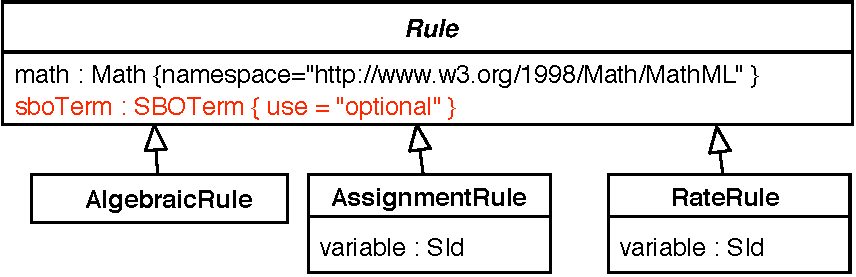
\includegraphics[scale = 0.68]{figs/rule}
  \caption{The definition of \Rule and derived types.
    Following UML notation fields
    that are inherited from a base class are not shown.}
  \label{fig:rules}
\end{figure}

\begin{blockChanged}
\subsubsection{The \token{sboTerm} Field}

The \Rule structure has an optional \token{sboTerm} field of type
\primtype{SBOTerm} (see Sections~\ref{sec:sboterm-type}
and~\ref{sec:sboTerm}).  This means that the object classes
derived from \Rule, namely \AlgebraicRule, \AssignmentRule, and
\RateRule, all have \token{sboTerm} fields.  When a value is given
to this field, it must be a valid SBO identifier referring to a
mathematical expression defined in SBO (\ie terms derived from
\sbomathformula).  The \AlgebraicRule, \AssignmentRule, or
\RateRule object should have a ``is a'' relationship with the SBO
term, and the term should be the most precise (narrow) term that
captures the role of that rule in the model.

As discussed in Section~\ref{sec:sboTerm}, SBO labels are optional
information on a model.  Applications are free to ignore
\token{sboTerm} values.  A model must be interpretable without the
benefit of SBO labels.

\end{blockChanged}


\subsubsection{\class{AlgebraicRule}}
\label{sec:algebraicrule}

The rule type \AlgebraicRule is used to express equations that are
neither assignments of model variables nor rates of change.
\AlgebraicRule does not add any fields to the basic \Rule;
its role is simply to distinguish this case from the other cases.  An
 example of the use of \AlgebraicRule structures is given in
Section~\ref{sec:algeraiceg}.


\subsubsection{\class{AssignmentRule}}
\label{sec:assignmentrule}

The rule type \AssignmentRule is used to express equations
that set the values of variables.  The left-hand side (the
\token{variable} field) of an assignment rule can refer to the
identifier of a species, compartment, or parameter \changed{(but
not a reaction)}.  Two or more \RateRule or
\AssignmentRule structures cannot have the same left-hand
side or \token{variable} field value in an SBML model definition.
In all cases, as would be expected, the units of the formula
representing the right hand side, the \token{math} field, are
identical to the units associated with the left hand side, the
\token{variable} field, when that variable appears in other
formulas.

The effects of an \AssignmentRule structure are in general terms
the same, but differ in the precise details depending on the type of variable
being set:
\begin{itemize}

\item \emph{In the case of a species}, an \AssignmentRule sets the
  referenced species' quantity (\quantity{concentration} or
  \quantity{amount of substance})
  to the value determined by the formula
  in \token{math}.  The units of the formula are the \emph{units of the species} as
  defined in Section~\ref{sec:species-units}.

  \emph{Restrictions}: In a given SBML Level~2 model, there cannot be both a
  \AssignmentRule \token{variable} field and a \SpeciesReference
  \token{species} field having the same
  value. (See Section~\ref{sec:reactions} for the definition of
  \SpeciesReference.)  This means an assignment rule cannot be
  defined for a species that is created or destroyed in a reaction.  The
  only exception is when the given species is a boundary condition; i.e.,
  on the \Species structure the
  \token{boundaryCondition} field is set to \val{true}.

\item \emph{In the case of a compartment}, an \AssignmentRule sets
  the referenced compartment's size to the size determined by the formula
  in \token{math}.  The overall units of the formula are the units
  specified for the size of the compartment identified by the value of the
  \AssignmentRule's \token{variable} field.  (See
  Section~\ref{sec:compartment-units} for an explanation of how the units of the
  compartment's size are determined.)

\item \emph{In the case of a parameter}, an \AssignmentRule sets the
  referenced parameter's value to that determined by the formula in
  \token{math}.  The overall units of the formula are the units
  defined for the parameter identified by the value of the
  \AssignmentRule's \token{variable} field.  (See
  Section~\ref{sec:parameter-units} for an explanation of how the units of the
  parameter are determined.)


\end{itemize}

\subsubsection{\class{RateRule}}
\label{sec:raterule}

The rule type \RateRule is used to express equations that
determine the rates of change of variables.  The left-hand side
(the \token{variable} of a rate rule) can refer to the identifier
of a species, compartment, or parameter \changed{(but not a
reaction)}. Two or more \RateRule or \AssignmentRule
structures cannot have the same left-hand side or
\token{variable} field value in an SBML model definition. In all
cases, as would be expected, the units of the formula representing
the right hand side, in the \token{math} field, are of the form
\quantity{x}/\quantity{time} where \quantity{x} are the same units
as associated with the symbol in the \token{variable} field, when
that variable appears in other formulas.  \quantity{time} is a
built-in unit (see Section~\ref{sec:unitdefinitions}). The effects
of a \RateRule are in general terms the same, but differ in
the precise details depending on which variable is being set:
\begin{itemize}

\item \emph{In the case of a species}, a \RateRule sets the rate of
  change of the species' quantity to the value determined by the
  formula in \token{math}.  The overall units of the formula must be
  \quantity{species quantity}/\quantity{time}, where the \quantity{time} units
  are the built-in units of time described in
  Section~\ref{sec:unitdefinitions} and the \quantity{species quantity} units
  are the \emph{units of the species} as
  defined in Section~\ref{sec:species-units}.

  \emph{Restrictions}: In a given model, there cannot be both a
  \SpeciesReference \token{species} field and a
  \RateRule \token{variable} field
  having the same
  value. (See Section~\ref{sec:reactions} for the definition of
  \SpeciesReference.)  \changed{This means an rate rule cannot be
  defined for a species that is created or destroyed in a reaction.}  The
  only exception is when the given species is a boundary condition; i.e.,
  on the \Species structure that defines the species the
  \token{boundaryCondition} field is set to \val{true}.

\item \emph{In the case of a compartment}, a \RateRule sets the rate
  of change of the compartment's size to the value determined by the
  formula in \token{math}.  The overall units of the formula are
  \quantity{size}/\quantity{time}, where the \quantity{time} units are the
  built-in units of time described in Section~\ref{sec:unitdefinitions} and
  the \quantity{size} units are the units of size on the compartment
  identified by the value of the \RateRule's \token{variable}
  field.  (See Section~\ref{sec:compartment-units} for an explanation of how the
  units of the compartment's size are determined.)

\item \emph{In the case of a parameter}, a \RateRule sets the rate
  of change of the parameter's value to that determined by the formula in
  \token{math}.  The overall units of the formula are of the form
  \quantity{x}/\quantity{time} where \quantity{x} are the units
  defined for the parameter identified by the value of the
  \AssignmentRule's \token{variable} field and the \quantity{time}
  units are the built-in units of time described in Section~\ref{sec:unitdefinitions}.  (See
  Section~\ref{sec:parameter-units} for an explanation of how the units of the
  parameter are determined.)

\end{itemize}

\subsubsection{Restrictions on Rules}
\label{sec:ruleconstraints}

\changed{
SBML specifically does not
stipulate the form of the algorithms that can be applied to rules
and reactions.  For example, SBML does not specify when or how
often rules should be evaluated.  The constraints described by
rules and kinetic rate laws are meant to apply collectively to the
set of variable values for a specific instant in time.
}

No more than one assignment or rate rule can be defined for a
given identifier.  No assignment or rate rule can be defined for
an identifier whose corresponding structure has the field
\token{constant} set to \token{true}.

\begin{blockChanged}
A rule cannot be used to set the value of a reaction rate; that
is, the value of a \token{variable} field in an \AssignmentRule or
\RateRule cannot be the value of any \Reaction's \token{id} field.

The value calculated by an \AssignmentRule object overrides the
value assigned to the given symbol by the object defining that
symbol.  For example, if a \Compartment's \token{size} is set in
its definition, and the model also contains an \AssignmentRule
having that compartment's \token{id} as its \token{variable}
value, then the interpretation is that the \token{size} assigned
in the \Compartment definition should be ignored and the value
assigned based on the computation defined in the
\AssignmentRule.

This does not mean that a definition of a symbol can be omitted if
there is an \AssignmentRule object for that symbol.  For
example, there must be a \Parameter definition for a given
parameter if there is an \AssignmentRule for that parameter.

A model must also not define initial assignments \emph{and}
assignment rules simultaneously for the same entity.  That is,
there cannot be \emph{both} an \AssignmentRule and an
\InitialAssignment for the same symbol in a model, because both
kinds of constructs apply at the start of simulated time and
allowing both to exist for a given symbol would result in
indeterminism.  (See also
Section~\ref{sec:initial-assignment-semantics}.)

The combined set of \InitialAssignment,
\AssignmentRule and \KineticLaw structures form a
set of assignment statements that should be considered as a whole.
The combined set of assignment statements should not contain
algebraic loops: a chain of dependency between these statements
should terminate. Formally consider the directed graph of
assignment statements where nodes are statements and directed arcs
exist for each occurrence of a symbol in an assignment statement
\token{math} field. The directed arcs start from the statement
assigning the symbol to the statements that contain the symbol in
their math fields. Such a graph must be acyclic. (A
\KineticLaw structure assigns to the symbol contained in
the \token{id} field of the containing \Reaction
structure).  Eliminating algebraic loops ensures that assignment
statements can be evaluated any number of times without the result
of those evaluations changing. As an example, consider the
following equations:
\begin{linenomath}
\begin{equation*}
  \begin{array}{lll}
    x = x + 1, & y = z + 200, & z = y + 100
  \end{array}
\end{equation*}
\end{linenomath}
If this set of equations were interpreted as a set of assignment
statements, it would be invalid because the rule for $x$ refers to
$x$ and the rule for $y$ refers to $z$ whilst the rule for $z$
refers to $y$.
\end{blockChanged}

The following set of equations if interpreted as assignment
statements would be valid:

\begin{linenomath}
\begin{equation*}
  \begin{array}{lll}
    x = 10, & y = z + 200, & z = x + 100
  \end{array}
\end{equation*}
\end{linenomath}

\begin{blockChanged}

A SBML model must not be overdetermined.  A SBML model that does
not contain \AlgebraicRule structures is not over
determined.

To determine whether a continuous deterministic mathematical model
is overdetermined we form a bipartite graph in which one set of
vertices represent the variables and the other the set of vertices
represent the equations. Edges in the graph link equation vertexes
to the variable vertices so that the variables are linked to the
equations that determine them. Edges connect each algebraic
equation vertex to all the vertices representing variables
occurring in the equation. For each an ordinary differential
equation (ODE) a single edge connects the vertex representing the
equation to the vertex representing the variable determined by the
equation.

A mathematical model is overdetermined if the maximal matchings
of the bipartite graph contain disconnected vertexes representing
equations. (If one maximal matching has this property then all the
maximal matchings will have this property i.e. it is only
necessary to find one maximal matching.)  A efficient algorithm
for finding a maximal matching is described in
\cite{hopcroft:1973}.)

We can define the application of the above general statement to
SBML by defining the mapping of SBML structures to components of
the bipartite graph representing the model structure. In this
mapping we consider assignment rules to be algebraic equations and
we consider the assignment of kinetic laws to reaction variables
to be algebraic equations.  We assume the construction of an ODE
for each species determined by one or more reaction rate laws. The
following mapping assumes that the model is valid in all respects
but may be overdetermined e.g. equations cannot refer to
undeclared variables.

The bipartite graph is formed as follows:
\begin{itemize}

\item Create equation vertexes for each of the following:

\begin{enumerate}
 \item a \Species structure that has the
 \token{boundaryCondition} field set to false and \token{constant}
field set to false and which is referenced by one or more reactant
or product lists of a \Reaction structure containing a
 \KineticLaw structure

\item a \Rule structure

\item a \KineticLaw structure
\end{enumerate}

\item Create variable vertexes for (a) every \Species,
 \Compartment and \Parameter structure which has the
 \token{Constant} field set to false; and (b) for every
 \Reaction structure.

\item Create an edge for each case of the following:

\begin{enumerate}
\item \emph{a \Species structure that has the
 \token{boundaryCondition} field set to false and \token{constant}
 field set to false and which is referenced by the reactant or
product lists of a \Reaction structure containing a
 \KineticLaw structure.} The edge connects the vertex
representing the species to the vertex representing the species'
equation (see (1) above)

\item \emph{an \AssignmentRule or \RateRule.} The
edge connects the vertex representing the \Rule to the
vertex representing the variable referenced by the
\token{variable} field of the rule.

\item \emph{a \KineticLaw.}  The edge connects the vertex
representing the \KineticLaw equation to the variable
vertex representing the \Reaction containing the
\KineticLaw.

\item \emph{the occurrence of a MathML \token{ci} symbol
referencing a variable (that is referencing a \Species,
\token{compartment}, \token{parameter} structure which has the
\token{constant} field set to false) within an
\AssignmentRule or \AlgebraicRule.} The edge
connects the vertex representing the rule to the vertex
representing the variable.

\item \emph{the occurrence of a MathML \token{ci} symbol
referencing a \Reaction within an \AssignmentRule or
\AlgebraicRule.}  The edge connects the vertex representing
the rule to the vertex representing the reaction variable.

\item \emph{the occurrence of a MathML \token{ci} symbol
referencing a variable within an \AssignmentRule or
\AlgebraicRule.} The edge connects the vertex representing
the rule to the vertex representing the variable.  The \token{ci}
element must either reference: (a) a \Species,
\token{compartment} or \token{parameter} structure which has the
\token{constant} field set to false; or (b) reference a
\Reaction structure)

\item \emph{the occurrence of a MathML \token{ci} symbol
referencing a variable within an \KineticLaw.} The edge
connects the vertex representing the kinetic law to the vertex
representing the variable.  The \token{ci} element must either
reference a \Species, \token{compartment} or
\token{parameter} structure which has the \token{constant} field
set to false.  In this context a \token{ci} element cannot refer
to a \Reaction structure.

\end{enumerate}
\end{itemize}
\end{blockChanged}

\subsubsection{Example of Rule Use}
\label{sec:eg-rule-use}

This section contains an example set of rules.  Consider the following
set of equations:
\begin{equation*}
  \begin{array}{lll}
    k = \D\frac{k_3}{k_2}, & s_2 = \D\frac{k \, x}{1 + k_2}, & A = 0.10 \, x
  \end{array}
\end{equation*}
This can be encoded by the following scalar rule set (where the definitions
of \texttt{x}, \texttt{s}, \texttt{k}, \texttt{k2}, \texttt{k3} and \texttt{A} are
assumed to be located elsewhere in the model and not shown in this
abbreviated example):

\begin{example}
    <listOfRules>
        <assignmentRule variable="k">
            <notes>
                <xhtml:p>
                    k = k3/k2
                </xhtml:p>
            </notes>
            <math xmlns="http://www.w3.org/1998/Math/MathML">
                <apply>
                    <divide/>
                    <ci> k3 </ci>
                    <ci> k2 </ci>
                </apply>
            </math>
        </assignmentRule>
        <assignmentRule variable="s2">
            <notes>
                <xhtml:p>
                    s2 = (k * x)/(1 + k2)
                </xhtml:p>
            </notes>
            <math xmlns="http://www.w3.org/1998/Math/MathML">
                <apply>
                    <divide/>
                    <apply>
                        <times/>
                        <ci> k </ci>
                        <ci> x </ci>
                    </apply>
                    <apply>
                        <plus/>
                        <cn> 1 </cn>
                        <ci> k2 </ci>
                    </apply>
                </apply>
            </math>
        </assignmentRule>
        <assignmentRule variable="A">
            <notes>
                <xhtml:p>
                    A = 0.10 * x
                </xhtml:p>
            </notes>
            <math xmlns="http://www.w3.org/1998/Math/MathML">
                <apply>
                    <times/>
                    <cn> 0.10 </cn>
                    <ci> x </ci>
                </apply>
            </math>
        </assignmentRule>
    </listOfRules>
\end{example}


%\subsubsection{Guidelines for Evaluating Rules}
%
%This section describes how rules including those implied by
%\Reaction structures (see Section~\ref{sec:reactions})
%should be evaluated.  For the purpose of interpreting models
%mathematically (and for this description), \Reaction
%structures collectively imply a \class{SpeciesConcentrationRule}
%structure, of type \class{rate}, for each species referenced in a
%\SpeciesReference structure excluding those species which
%are defined with the \token{boundaryCondition} attribute equal to
%\texttt{true}.
%
%To determine the initial values of variables is a 2 set process:
%
%\begin{itemize}
%
%\item variables should be set according to the initial values
%given by \Species, \Compartment and
%\Parameter structures then
%
%\item the \class{scalar} rules should be evaluated
%
%\end{itemize}
%
%To determine the rates of change of variables given a set of
%current variable values is again a two set process:
%
%\begin{itemize}
%
%\item the \class{scalar} rules should be evaluated then
%
%\item the \class{rate} rules should be evaluated
%
%\end{itemize}
%
%The \class{scalar} rules should be evaluated to determine the
%complete set of variable values given an incomplete set of
%variable values determined by \class{rate} and
%\AlgebraicRule structures.
%

\begin{blockChanged}
%-----------------------------------------------------------------------------
\subsection{Constraints}
\label{sec:constraints}
%-----------------------------------------------------------------------------

The \Constraint structure is a mechanism for stating the
assumptions under which a model is designed to operate.  The
\emph{constraints} are statements about permissible values of
different quantities in a model.  Figure~\vref{fig:constraint}
shows the definition of the \Constraint data structure.

\begin{figure}[htb]
  \begin{blockMarkChanged}
  \centering
  \small
  \begin{classbox}{Constraint}
    sboTerm: SBOTerm \{ use="optional" \}                                                            \\
    math: Math \{ namespace="http://www.w3.org/1998/Math/MathML" \}                                  \\
    message: (ANY: \{ namespace="http://www.w3.org/1999/xhtml" \}) \{ minOccurs="0" maxOccurs="1" \} \\
  \end{classbox}
  \caption{The definition of \Constraint.
    Following UML notation fields
    that are inherited from a base class are not shown.}
  \label{fig:constraint}
  \end{blockMarkChanged}
\end{figure}

A \Constraint structure consists of two fields:
\token{math}, which contains a MathML formula, and the optional
field \token{message}, which contains a message in XHTML format that may
be displayed to the user.  The formula contained in the
\token{math} field should be an arbitrary function of the
variables and parameters of the SBML model.  The formula must
return a boolean value of \texttt{true} when the model is a
\emph{valid} state.  \Constraint structures have effect at
all times, i.e, $t >= 0$.

\Constraint structures \emph{cannot and should not} be used
to compute the dynamical behavior of a model as part of, for
example, simulation. They simply provide a mechanism allowing a
modeler to express the validity of a model's state during
numerical analysis.  Constraints may be used as a key input to
non-dynamical analysis, for example by expressing flux constraints
for flux balance analysis.

The results of a simulation of a model containing a constraint are
invalid from any simulation time at and after a point when the
function given by the \token{math} returns a value of
\val{false}. (Invalid simulation results do not make a
prediction of the behavior of the biochemical reaction network
represented by the model.)  The precise behavior of simulation
tools is left undefined with respect to constraints. If invalid
results are detected with respect to a given constraint, the
\token{message} field may optionally be displayed to the user.
Software tools are not required to display the message, but it is
recommended as a matter of best practice. The simulation tool may
also halt the simulation or clearly delimit in output data the
simulation time point at which the simulation results become
invalid.


\subsubsection{The \token{sboTerm} Field}

The \Constraint structure has an optional \token{sboTerm} field of
type \primtype{SBOTerm} (see Sections~\ref{sec:sboterm-type}
and~\ref{sec:sboTerm}).  When a value is given to this field in a
constraint definition, the value must be a valid SBO identifier
referring to a mathematical expression (\ie terms derived from
\sbomathformula).  The \Constraint should have an ``is a''
relationship with the SBO term, and the term should be the most
precise (narrow) term that captures the role of the
\Constraint in the model.

As discussed in Section~\ref{sec:sboTerm}, SBO labels are optional
information on a model.  Applications are free to ignore
\token{sboTerm} values.  A model must be interpretable without the
benefit of SBO labels.


\subsubsection{Example}

As an example, the following SBML fragment demonstrates the
constraint that species $S_1$ should only have values between 1
and 100:

\begin{example}
<listOfConstraints>
    <constraint>
        <math xmlns="http://www.w3.org/1998/Math/MathML">
            <apply>
                <and/>
                <apply>
                    <lt/>
                    <cn> 1 </cn>
                    <ci> S1 </ci>
                </apply>
                <apply>
                    <lt/>
                    <ci> S1 </ci>
                    <cn> 100 </cn>
                </apply>
            </apply>
        </math>
        <message>
            <p xmlns="http://www.w3.org/1999/xhtml">
                Species S1 is out of range
            </p>
        </message>
    </constraint>
</listOfConstraints>
\end{example}

\end{blockChanged}


%-----------------------------------------------------------------------------
\subsection{Reactions}
\label{sec:reactions}
%-----------------------------------------------------------------------------

A \emph{reaction} represents any transformation, transport or binding
process, typically a chemical reaction, that can change the
amount of one or more species.  In SBML, a reaction is defined primarily in
terms of the participating reactants and products (and their corresponding
stoichiometries), along with optional modifier species, an optional kinetic
law describing the rate at which the reaction takes place, and optional
parameters entering into the kinetic law.  These various parts of a
reaction are recorded in the SBML \Reaction type defined in
Figure~\vref{fig:reaction}.

\begin{figure}[htb]
  \centering
  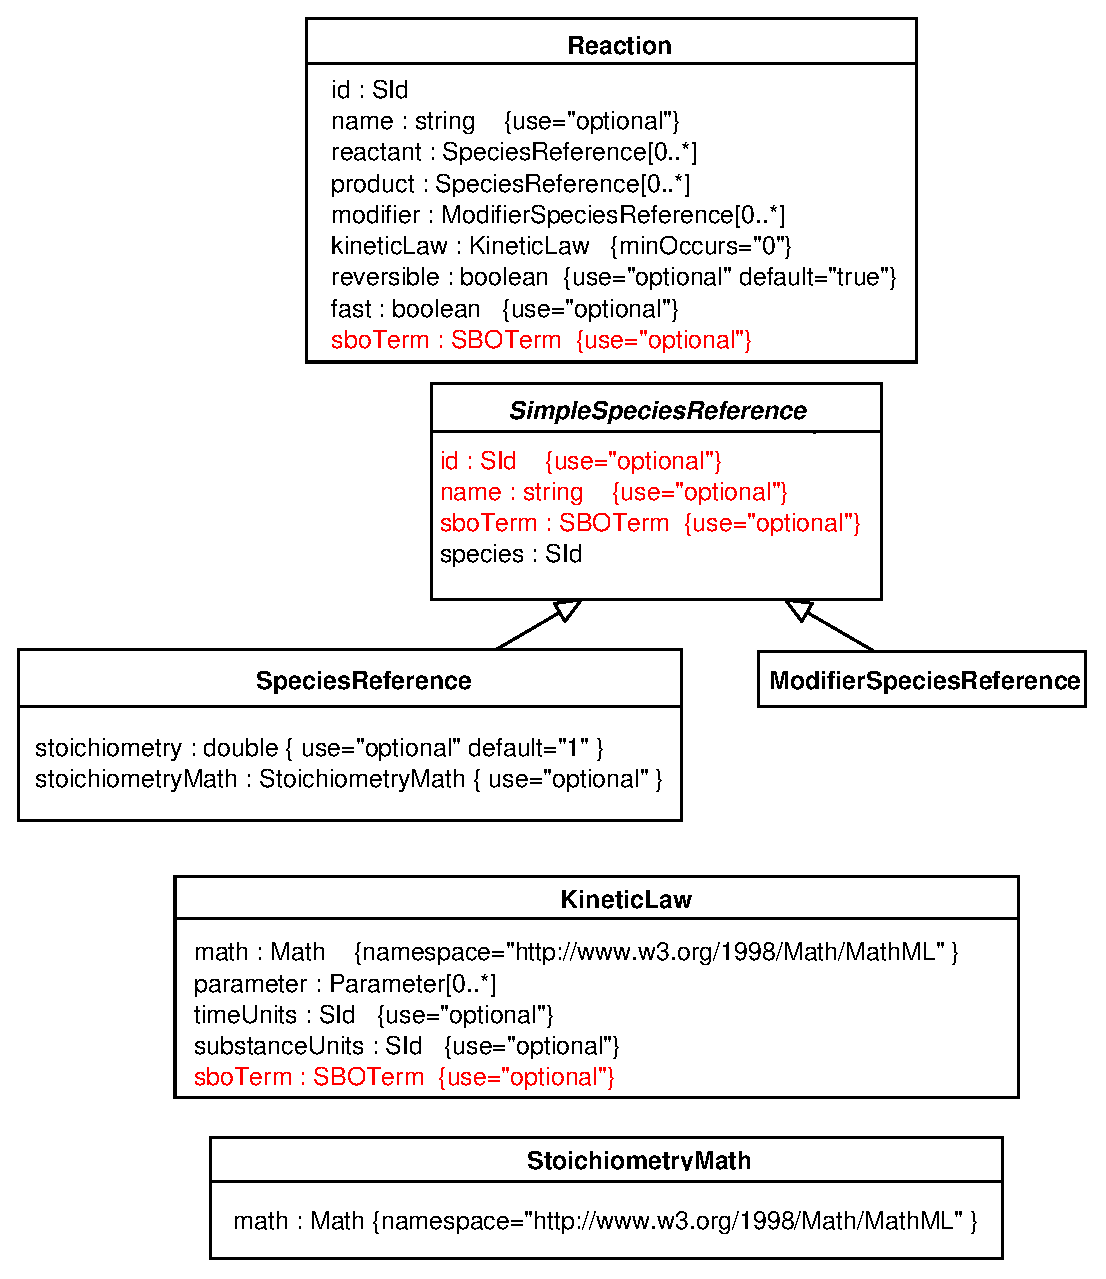
\includegraphics[scale=0.67]{figs/reaction}
  \caption{The definitions of \Reaction, \KineticLaw,
    \SpeciesReference and \ModifierSpeciesReference.
    Following UML notation fields
    that are inherited from a base class are not shown.}
  \label{fig:reaction}
\end{figure}


\subsubsection{The \token{id} and \token{name} Fields}

As with most other main structures in SBML, the \Reaction data
structure includes a required \token{id}\changed{, of type
  \primtype{SId},} and an optional \token{name}\changed{, of type
  \primtype{string}}.  These must be used according to the
guidelines described in Section~\ref{sec:idnameattribs}.

\begin{blockChanged}
The identifier of a \Reaction structure can be used in mathematical
formulas in an SBML model to represent the rate of the reaction.  This
usage is explained in detail in Section~\ref{subsec:reaction-as-symbol}
below.
\end{blockChanged}


\subsubsection{The \token{reactant}, \token{product} and \token{modifier} Fields}

\begin{blockChanged}
The reactant species, product species and
modifier species in a reaction are described using the fields
\token{reactant}, \token{product} and \token{modifiers}, respectively.
These fields are optional lists of \SpeciesReference and
\ModifierSpeciesReference structures, as shown in
Figure~\vref{fig:reaction}.  They are described in more detail in
Sections~\ref{subsec:speciesreference} and~\ref{subsec:modifierreference}
below.
\end{blockChanged}


\subsubsection{The \token{reversible} Field}

The optional boolean field \token{reversible} indicates
whether the reaction is reversible.  The field is optional, and if left
unspecified in a model, it defaults to a value of \val{true}.
Although the reversibility of a reaction is determined by its rate law, the
need to allow rate expressions in SBML to be optional leads to the need for
a \changed{separate} flag indicating reversibility.  Information about reversibility in the
absence of a \token{KineticLaw} in a \Reaction is useful in certain
kinds of structural analyses such as elementary mode analysis.  It is true
that the presence of this information in two places (i.e., the rate
expression and the flag \token{reversible}) leaves open the possibility of
a model containing contradictory information, but the creation of such a
model would indicate an error on the part of the software generating it.
Software developers must take care to guard against logical contradictions
in the definitions of reactions.

\begin{blockChanged}
\subsubsection{The \token{fast} Field}

The optional boolean field \token{fast} is another optional
boolean field in the \Reaction data structure.  The field has no
default value.

Previous definitions of SBML indicated that software tools could
ignore this field if they did not implement support for the
corresponding concept; however, further research has revealed that
this is incorrect and \token{fast} cannot be ignored.  \sbmltwotwo
stipulates that if a model has values for \token{fast}, a software
tool must be able to respect the field or else indicate to the
user that it does not have the capacity to do so.

When a model contains values for \token{fast} on any of its
reactions, it is an indication that the creator of the model is
distinguishing different time scales of reactions.  The model's
reaction definitions are divided into two sets by the values of
the \token{fast} fields.  The set of reactions which have values
of \val{true} (known as \emph{fast reactions}) should be assumed
to be operating on a time scale significantly faster than the
other reactions (the \emph{slow reactions}).  Fast reactions are
considered to be instantaneous relative to the slow reactions.
Software tools must use a pseudo steady-state approximation for
the set of fast reactions when constructing the system of
equations for the model.

Modelers should take care to note that the correctness of the
approximation requires a significant separation of time scales
between the fast reactions and other proceses.  This is not
trivial to estimate a priori, and may even change over the course
of a simulation, but can be reasonably assessed a posteriori in
most cases.

Care must be taken when interpreting values on the \token{fast}
field.  The absence of a default value means that if a there are
\emph{no} values for \token{fast} anywhere in a model, the field
itself cannot be used to make assumptions about fast or slow
reactions; it only means the creator of the model is not using the
field to make time scale distinctions.  If the model does in fact
constain fast reactions, they may be represented in another way.
Conversely, if a model \emph{does} contain a value for
\token{fast} on any reaction, then the model's creator is making
explicit statements about time scale separations and software
reading the model must take appropriate steps or risk
misinterpreting the model.  Since there is no default value, the
best-practice recommendation is to label all reactions in a model
(either \val{true} or \val{false}) if any one of the reactions
needs to be given a value.

Analysis software cannot ignore the value of the \token{fast}
attribute because doing so may lead to different results when
compared to a software system that makes use of \token{fast}.  For
maximal interoperability, we recommend that SBML models are not
generated with the \token{fast} attribute set to \val{true};
instead, any approximation required by the model should be made
explicit through the use of rules (see Section~\ref{sec:rules}).


%This may be relevant when computing equilibrium concentrations of
%rapidly equilibrating reactions.  Simulation/analysis packages may
%chose to use this information to reduce the number of ODEs
%required and thereby optimize such computations.

% Mike the following is exactly what the guys at Virtual Cell are
% saying is not possible.  They said software that didn't do
% transformation to PSST and just ignored true values would get the wrong
% results....
%
%(A simulator/analysis package that has no facilities for dealing
%with fast reactions can ignore this field. In theory, if the
%choice of which reactions are fast is correctly made, then a
%simulation performed with them should give the same results as a
%simulation performed without fast reactions. However, currently
%there appears to be no single unambiguous method for designating
%which reactions should be considered fast, and some users may
%designate a reaction as fast when in fact it is not.)


\subsubsection{The \token{sboTerm} Field}

The \Reaction structure has an optional \token{sboTerm} field of
type \primtype{SBOTerm} (see Sections~\ref{sec:sboterm-type}
and~\ref{sec:sboTerm}).  When a value is given to this field in a
reaction definition, the value must be a valid SBO identifier
referring to a modeling framework (\ie terms derived from
\sboframework).  The \Reaction structure should have an ``is a''
relationship with the SBO term.  The SBO term chosen should be the
most precise (narrow) term that defines the mathematical framework
used in the reaction.

As discussed in Section~\ref{sec:model-sboterm}, the value given
to \token{sboTerm} on a model's \Reaction objects interacts with
the SBO labels on the \Model element.  If the \Model's
\token{sboTerm} field has a value, it should be interpreted to
mean that all the reactions in a model assume the same modeling
framework.  In that case, the \token{sboTerm} labels on individual
reactions may be omitted, but only the \Reaction SBO labels can be
thus omitted; the SBO labels on \KineticLaw within \Reaction must
still be supplied, as must the terms on other components of the
model, in order to characterize the model completely.  (See
Section~\ref{sec:model-sboterm} for more discussion about this
topic.)

SBO labels are optional information on a model.  Applications are
free to ignore \token{sboTerm} values, and a model must be
interpretable without the benefit of SBO labels.
Section~\ref{sec:sboTerm} gives more information about this
principle and the use of SBO.


\subsubsection{\abstractclass{SimpleSpeciesReference}}
\label{subsec:simplespeciesreference}

Every species that enters into a given reaction must appear in
that reaction's lists of reactants, products \changed{and/or} modifiers.  In an
SBML model, all species that \changed{may} participate in any reaction are
listed in the \token{listOfSpecies} field of the top-level
\Model data structure (see Section~\ref{sec:model}).  Lists
of products, reactants and modifiers in \Reaction
structures do not introduce new species, but rather, they refer
back to those listed in the model's top-level \token{listOfSpecies}.  For
reactants and products, the connection is made using the
\SpeciesReference data structure; for modifiers, it is made
using the \ModifierSpeciesReference data structure.

\SimpleSpeciesReference, defined in Figure~\vref{fig:reaction}, is
an abstract type that serves as the parent class of both
\SpeciesReference and \ModifierSpeciesReference.  It is used
simply to hold the fields \token{species}, \token{id},
\token{name}, and \token{sboTerm} that are common to the latter
structures.


\paragraph{The \token{id} and \token{name} Fields}

The optional identifier stored in the \token{id} field allows the
\abstractclass{SimpleSpeciesReference} structure to be referenced
from other structures.  There are as yet no SBML structures that
do this; however, such structures are anticipated in future levels
of SBML.  The identifier must be a text string conforming to the
syntax permitted by the \primtype{SId} data type described in
Section~\ref{sec:sid}.  The \token{id} value (whether it is in a
\SpeciesReference or \ModifierSpeciesReference object) exists in
the global namespace of the model, as described in
Section~\ref{sec:idnameattribs}.  \SimpleSpeciesReference also has
an optional \token{name} field, of type \primtype{string}.  The
\token{name} and \token{id} fields must be used as described in
Section~\ref{sec:idnameattribs}.


\paragraph{The \token{sboTerm} Field}

The \SimpleSpeciesReference structure has an optional
\token{sboTerm} field of type \primtype{SBOTerm} (see
Sections~\ref{sec:sboterm-type} and~\ref{sec:sboTerm}).  This
means that the object classes derived from
\SimpleSpeciesReference, namely \SpeciesReference and
\ModifierSpeciesReference, all have \token{sboTerm} fields.  When
a value is given to this field, it must be a valid SBO referring
to a participant role.  The appropriate term depends on whether
the object is a reactant, product or species.  If a reactant, then
it should be a term in the \sboreactant hierarchy; if a product,
then it should be a term in the \sboproduct hierarchy; and if a
modifier, then it should be a term in the \sbomodifier hierarchy.
The \SpeciesReference and \ModifierSpeciesReference structures
should have an ``is a'' relationship to the term identified by the
SBO term identifier.  The SBO terms chosen should be the most
precise (narrow) one that defines the role of the species in the
reaction.

A product term must only be used when the \SpeciesReference
structure is contained in the \token{product} field of the
containing \Reaction structure.  Similarly, a reactant term must
only be used when the \SpeciesReference structure is contained in
the \token{reactant} field of the containing \Reaction structure.

As discussed in Section~\ref{sec:sboTerm}, SBO labels are optional
information on a model.  Applications are free to ignore
\token{sboTerm} values.  A model must be interpretable without the
benefit of SBO labels.


\end{blockChanged}


\subsubsection{\SpeciesReference}
\label{subsec:speciesreference}

\begin{blockChanged}
In a given reaction, references to a model's species that act as reactants
and/or products are made using \SpeciesReference data objects.

\paragraph{The \token{species} field}

The mandatory field \token{species}, inherited from
\SimpleSpeciesReference (Section~\ref{subsec:simplespeciesreference}),
must refer to the name of an existing species defined in the enclosing
\Model structure.
\end{blockChanged}

\paragraph{The \token{stoichiometry} and \token{stoichiometryMath}
fields}

\changed{Product and reactant
stoichiometries can be specified using \emph{either} \token{stoichiometry} or
\token{stoichiometryMath} in the \SpeciesReference structure.}
The \token{stoichiometry} field is of type double and should contain values
greater than 0. The \token{stoichiometryMath} field is implemented as an
element containing a MathML math expression in dimensionless units.  Only
one of the \token{stoichiometry} and \token{stoichiometryMath} fields
should be used on a given \SpeciesReference structure.  When neither
field is present then the stoichiometry associated with the
\SpeciesReference structure is ``\token{1}''.

\changed{For maximum interoperability between models and software tools,
we recommend that when generating SBML Level 2 models,
the \token{stoichiometry} field be used} in
preference to the \token{stoichiometryMath} field and that the
\token{stoichiometry} field contains integer values.  Parsing
software should expect and handle appropriately all possible
values of the \token{stoichiometry} and
\token{stoichiometryMath} fields including, for example,
non-integer values for \token{stoichiometry}. \changed{The
expression in \token{stoichiometryMath} may refer to species
identifiers, as discussed in Section~\ref{sec:ci-token}.  The only
species identifiers that can be used in \token{stoichiometryMath}
are those listed in the \token{reactant}, \token{product} and
\token{modifier} fields of the containing \Reaction
structure.}

The following is a simple example of a species reference for species
``X0'', with stoichiometry 2, in a list of reactants within a reaction
named ``J1'':

\begin{example}
<model>
    ...
    <listOfReactions>
        <reaction id="J1">
            <listOfReactants>
                <speciesReference species="X0" stoichiometry="2">
            </listOfReactants>
            ...
        </reaction>
        ...
    </listOfReactions>
    ...
</model>
\end{example}

The following is a more complex example of a species reference for species
``X0'', with a stoichiometry expression consisting of the parameter \texttt{x}:

\begin{example}
<model>
    ...
    <listOfReactions>
        <reaction id="J1">
            <listOfReactants>
                <speciesReference species="X0">
                    <stoichiometryMath>
                        <math xmlns="http://www.w3.org/1998/Math/MathML">
                            <ci>x</ci>
                        </math>
                    </stoichiometryMath>
                </speciesReference>
            </listOfReactants>
            ...
        </reaction>
        ...
    </listOfReactions>
    ...
</model>
\end{example}

%A reaction can contain an empty list of reactants or an empty list of
%products but must have at least one reactant or product.  Also note that
%whether a given species is allowed to appear as a reactant or product is
%dictated by certain flags on the structure defining the species in the
%model; see Section~\ref{sec:species-constant} for more information.

A species can occur more than once in the lists of reactants and
products of a given reaction.  The effective stoichiometry for a
species in a reaction is the sum of the stoichiometry values given
on the \SpeciesReference structures in the list of products minus
the sum of stoichiometry values given on the \SpeciesReference
structures in the list of reactants.  A positive value indicates
the species is effectively a product and a negative value
indicates the species is effectively a reactant.  SBML places no
restrictions on the effective stoichiometry of a species in a
reaction; for example, it can be zero.  In the following SBML
fragment, the two reactions have the same effective stoichiometry
for all their species:

\begin{example}
<reaction id="x">
    <listOfReactants>
        <speciesReference species="a"/>
        <speciesReference species="a"/>
        <speciesReference species="b"/>
    </listOfReactants>
    <listOfProducts>
        <speciesReference species="c"/>
        <speciesReference species="b"/>
    </listProducts>
</reaction>
<reaction id="y">
    <listOfReactants>
        <speciesReference species="a" stoichiometry="2"/>
    </listOfReactants>
    <listOfProducts>
        <speciesReference species="c"/>
    </listProducts>
</reaction>
\end{example}

\paragraph{Constraints on the use of \class{SpeciesReference}
structures}

A reaction can contain an empty list of reactants or an empty list
of products but must have at least one reactant or product.  Also
note that whether a given species is allowed to appear as a
reactant or product is dictated by certain flags on the structure
defining the species in the model; see
Section~\ref{sec:species-constant} for more information.

\subsubsection{\ModifierSpeciesReference}
\label{subsec:modifierreference}

\begin{blockChanged}
Sometimes a species appears in the kinetic rate formula of a reaction but
is itself neither created nor destroyed in that reaction (for example,
because it acts as a catalyst or inhibitor).  In SBML, all such species are
simply called \emph{modifiers} without regard to the detailed role of
those species in the model.
The \Reaction structure provides a way to express which
species act as modifiers in a given reaction.  This is the purpose
of the \token{modifier} field in \Reaction; this field is
a list of \ModifierSpeciesReference structures defined in
Figure~\vref{fig:reaction}.

The \ModifierSpeciesReference structure has a mandatory
field, \token{species}, of type \primtype{SId}, inherited from
\SimpleSpeciesReference; its value must be the identifier
of a species defined in the enclosing \Model.   This
species is designated as a modifier for the current reaction.  A
reaction may have any number of modifiers.  The
\ModifierSpeciesReference structure also has an
optional field named \token{id}, used to give the reference an
identifier.  The identifier must be a text string conforming to
the syntax permitted by the \primtype{SId} data type described in
Section~\ref{sec:sid}.  The \token{id} value exists in the global
namespace of the model as described in
Section~\ref{sec:idnameattribs}.  \ModifierSpeciesReference
also has an optional \token{name} field, of type \primtype{string}.
The \token{name} and \token{id} fields \changed{must} be used as
described in Section~\ref{sec:idnameattribs}.

It is permissible for a modifier species to simultaneously appear in the
list of reactants and products of the same reaction where it is
designated as a modifier, as well as to appear in the list of reactants,
products and modifiers of other reactions in the model.

\end{blockChanged}


\subsubsection{\KineticLaw}
\label{subsec:kinetic-law}

A \token{kineticLaw} structure, enclosed in a \Reaction structure,
 describes the rate at which the reaction
takes place.  The inclusion of a \KineticLaw structure in an
instance of a \Reaction component is optional; however, in general
there is no useful default that can be substituted in place of a missing
rate law definition in a reaction.

\paragraph{The \token{math} field}

As shown in Figure~\vref{fig:reaction}, the \KineticLaw structure has a
field called \token{math}; this is a MathML expression  defining the
rate of the reaction.

It is important to make clear at the outset that a ``kinetic law'' in SBML
is \emph{not} equivalent to a traditional rate law.  The reason is that
SBML must support multi-compartment models, and the units used in textbook
rate laws as well as some conventional single-compartment modeling packages
are problematic when used for defining reactions between multiple
compartments.  Rate expressions in SBML are expressed in terms of
\quantity{substance}/\quantity{time}, rather than the more typical
\quantity{concentration}/\quantity{time}.  Converting between these two
conventions is a simple matter of dividing the
\quantity{substance}/\quantity{time} expression by the size of the
compartment where a given species is located.  To put this in slightly more
precise terms, suppose there are two species $S$ and $P$ in a reaction
$S \rightarrow P$, where $S$ is located in a compartment $A$ having
volume $V_A$, $P$ is located in a compartment $B$ having volume $V_B$, and
the kinetic law expression gives the rate of the reaction as being $R$.
Then the rate of change in the concentration of $S$ is given by $d[S]_A/dt
= -R/V_A$ and the rate of change in the concentration of $P$ is $d[P]_B/dt
= R/V_B$.  The translation of a complete multi-compartmental model into
ODEs is given in Section~\ref{sec:odeeg}.

\changed{The expression in \token{math} may refer to species
identifiers, as discussed in Section~\ref{sec:ci-token}.}  The
only species identifiers that can be used in \token{math} are
those listed in the \token{species} fields  of the
\token{reactant}, \token{product} and \token{modifier} structures
contained in the \Reaction structure.

\paragraph{The \token{substanceUnits} and \token{timeUnits}
fields}

As previously stated, the overall rate expression in the
\token{math} field must have the units of
\quantity{substance/time}.  The optional fields
\token{substanceUnits} and \token{timeUnits} determine the units
of substance and time for the reaction, respectively. The values
of these fields must be chosen from one of the following
possibilities: one of the base unit names from
Table~\vref{tab:unitkind}; one of the built-in unit names
appearing in the first column of Table~\vref{tab:builtin}); or the
name of a new unit defined in the list of unit definitions in the
enclosing \Model structure.  \changed{In the case of
\token{substanceUnits}, the value chosen must be a scaled and/or
multiplied variant of \token{dimensionless}, \token{moles}, or
\token{item}. In the case of \token{timeUnits}, the value chosen
must be a scaled and/or multiplied variant of \token{seconds} or
\token{dimensionless}, with an \token{exponent} field value of
\val{1}.}. If these fields are not set in a given \KineticLaw
instance, the units are taken from the defaults defined by the
built-in ``\token{substance}'' and ``\token{time}'' of
Table~\vref{tab:builtin}.

\paragraph{The \token{Parameter} field}

An instance of a \KineticLaw type structure can contain zero or more
\token{parameter} structures (Section~\ref{sec:parameters}) which define
symbols that can be used in the \token{math} field.  As discussed in
Section~\ref{sec:identifiers}, reactions introduce local namespaces for
parameter identifiers.  Within a \KineticLaw structure inside a
reaction definition, a local parameter whose identifier is identical to a
global parameter defined in the enclosing \Model-type structure
takes precedence over that global parameter.

\paragraph{The \token{sboTerm} field}

\begin{blockChanged}
The \KineticLaw structure has an optional \primtype{SBOTerm}
field, \token{sboTerm} (see Section~\ref{sec:sboTerm}).  This
field when present must contain a Systems Biology Ontology
(SBO; \sboref) term identifier referring to a kinetic law SBO term,
that is a term derived from \sboratelaw.  The
\KineticLaw structure should have a `is a' relationship
with the SBO term. The SBO term chosen should be the most precise
(narrow) term that defines the type of kinetic law encoded by the
structure.

\paragraph{Example}

The following is an example of a \Reaction structure that
defines a reaction named $J_1$, in which $X_0 \rightarrow S_1$ at
a rate given by $k X_0 S_2$, in conventional units, where $S_2$ is
a catalyst and $k$ is a parameter.  It demonstrates the use of
species references and the \KineticLaw structure.  The
units on the species here are the defaults of
\quantity{substance}/\quantity{volume} (see
Section~\ref{sec:species}), and so the conventional rate
expression is multiplied by the compartment volume so that the
encoded rate expression has the final units of
\quantity{substance/time}.

\begin{example}

<model>
    ...
    <listOfUnitDefinitions>
        <unitDefinition id="concent_per_time">
            <listOfUnits>
                <unit kind="litre"/>
                <unit kind="mole"   exponent="-1"/>
                <unit kind="second" exponent="-1"/>
            </listOfUnits>
        </unitDefinition>
    </listOfUnitDefinitions>
    ...
    <listOfSpecies>
        <species id="S1" compartment="c1" initialConcentration="2.0"/>
        <species id="S2" compartment="c1" initialConcentration="0.5"/>
        <species id="X0" compartment="c1" initialConcentration="1.0"/>
    </listOfSpecies>
        ...
    <listOfReactions>
        <reaction id="J1">
            <listOfReactants>
                <speciesReference species="X0"/>
            </listOfReactants>
            <listOfProducts>
                <speciesReference species="S1"/>
            </listOfProducts>
            <listOfModifiers>
                <modifierSpeciesReference species="S2"/>
            </listOfModifiers>
            <kineticLaw>
                <math xmlns="http://www.w3.org/1998/Math/MathML">
                    <apply>
                        <times/>
                        <ci> k </ci>
                        <ci> S2 </ci>
                        <ci> X0 </ci>
                        <ci> c1 </ci>
                    </apply>
                </math>
                <listOfParameters>
                    <parameter id="k" value="0.1" units="concent_per_time"/>
                </listOfParameters>
            </kineticLaw>
        </reaction>
    </listOfReactions>
    ...
</model>
\end{example}
\end{blockChanged}


\begin{blockChanged}
\subsubsection{Reaction Identifiers Used in Mathematical Expressions}
\label{subsec:reaction-as-symbol}

The value of the \token{id} field of a \Reaction structure
can be used as the content of a MathML \token{ci} element. Such a
\token{ci} element or symbol represents the rate of the given
reaction as given by the \KineticLaw structure of the
reaction.  The symbol has the units of the \KineticLaw as
described in Section~\ref{subsec:kinetic-law} or
\quantity{substance/time} units if the \KineticLaw is not
present.

A \KineticLaw structure forms an assignment statement
assigning the evaluated value of the \token{math} field to the
symbol value contained in the \Reaction \token{id} field.
No other structure can assign a value to such a reaction symbol;
i.e., the \token{variable} fields of \InitialAssignment,
\RateRule, \AssignmentRule and
\EventAssignment structures cannot contain the value of a
\Reaction \token{id} field.

The combined set of \InitialAssignment, \AssignmentRule and
\KineticLaw structures form a set of assignment statements that
should be considered as a whole.  The combined set of assignment
rules should not contain algebraic loops: a chain of dependency
between these statements should terminate.  (More formally,
consider the directed graph of assignment statements where nodes
are statements and directed arcs exist for each occurrence of a
symbol in a assignment statement \token{math} field. The directed
arcs start from the statement defining the symbol to the
statements that contain the symbol in their math fields. Such a
graph must be acyclic.)  Examples of valid and invalid set of
assignment statements are given in
Section~\ref{sec:ruleconstraints}.

\end{blockChanged}


%-----------------------------------------------------------------------------
\subsection{Events}
\label{sec:events}
%-----------------------------------------------------------------------------

\Model has an optional list of \Event structures that
describe the time and form of explicit instantaneous discontinuous state
changes in the model.  For example, an event may describe that one species
concentration is halved when another species concentration exceeds a given
threshold value.

An \Event structure defines when the event can occur, the variables
that are affected by the event, and how the variables are affected.  The
effect of the event can optionally be delayed after the occurrence of the
condition which invokes it.  The operation of an \Event structure is
divided into two phases (even when the event is not delayed): one when the
event is \emph{fired} and the other when the event is \emph{executed}. The
\Event type is defined in Figure~\vref{fig:event}.  Both
\Event and \EventAssignment are derived from \SBase
(see Section~\ref{sec:sbase}).  An example of a model which uses events is
given below.

\begin{figure}[htb]
  \centering
  \begin{classbox}{Event}
    id: SId                                                                     \\
    name: string \{ use="optional" \}                                           \\
    trigger: (math : Math \{ namespace="http://www.w3.org/1998/Math/MathML" \}) \\
    delay: (math : Math \{ namespace="http://www.w3.org/1998/Math/MathML" \}) \{ minOccurs="0" maxoccurs="1" \} \\    
    timeUnits: SId \{ use="optional" \}                                         \\
    \markChanged{sboTerm: SBOTerm \{ use="optional" \}}                             \\
    eventAssignment: EventAssignment[1..*]                                      \\
  \end{classbox}
  \vspace*{2ex}
  \begin{classbox}{EventAssignment}
    variable: SId                                                              \\
    \markChanged{sboTerm: SBOTerm \{ use="optional" \}}                            \\
    math: Math \{ namespace="http://www.w3.org/1998/Math/MathML" \}            \\
  \end{classbox}
  \caption{The definitions of \Event and \EventAssignment.
    Following UML notation, additional fields that are inherited
    from a base class, in this case \SBase, are not shown.}
  \label{fig:event}
\end{figure}


\begin{blockChanged}
\subsubsection{\class{Event}}

An \Event definition has three required parts: an identifier, a
trigger condition and at least one \EventAssignment. In addition
there is an optional delay expression.  These are described below.
\end{blockChanged}


\paragraph{The \token{id} and \token{name} Fields}
\label{sec:event-id-name}

These optional fields are available to support external references
to event structures.  These fields operate in the manner described in
Section~\ref{sec:idnameattribs} except that the \token{id} field is optional.


\paragraph{The \token{trigger} Field}
\label{sec:event-trigger}

The \token{trigger} field defines when the \Event structure has an
effect on the model.  The \token{trigger} field contains a MathML boolean
expression.  The exact instant that the expression evaluates to true is the
time point when the \Event is \emph{fired}.  The event only fires
when the \token{trigger} makes the transition from false to true.  The
event will fire at any further time points when the \token{trigger} make
this transition.


\paragraph{The \token{delay} Field}
\label{sec:event-delay}

The optional \token{delay} field defines the length of time after
the event has \emph{fired} that the event is \emph{executed}. The
\token{delay} field is another MathML expression.  This
expression should be evaluated when the rule is \emph{fired}.  The
default value for the \token{delay} field is 0.  The value of the
\token{delay} field should always be positive.  The units of the \token{delay}
field are those given on the \token{timeUnits} field.


\paragraph{The \token{timeUnits} Field}
\label{sec:event-timeunits}

The optional field \token{timeUnits} determines the units of time
that apply to the \token{delay} field.
The value of the \token{timeUnits} field must be either
``\token{second}'' or ``\token{dimensionless}'' from Table~\vref{tab:unitkind}, ``\token{time}'' from
Table~\vref{tab:builtin},
or a new unit defined by a unit definition in the enclosing model
which must be a variant of ``\token{second}'' units.
The default value of the \token{timeUnits} field is
``\token{time}''.


\begin{blockChanged}
\paragraph{The \token{sboTerm} Field}

The \Event structure has an optional \token{sboTerm} field of type
\primtype{SBOTerm} (see Sections~\ref{sec:sboterm-type}
and~\ref{sec:sboTerm}).  The term is associated with the trigger
condition on the event.  When a value is given to this field, it
must be a valid SBO referring to a mathematical expression (\ie
terms derived from \sbomathformula).  The \Event's trigger should
have a ``is a'' relationship with the SBO term, and the term
should be the most precise (narrow) term that captures the form of
the trigger formula in the model.

As discussed in Section~\ref{sec:sboTerm}, SBO labels are optional
information on a model.  Applications are free to ignore
\token{sboTerm} values.  A model must be interpretable without the
benefit of SBO labels.

\end{blockChanged}


\paragraph{The \token{eventAssignment} Field}
\label{sec:eventassignment}

The \token{eventAssignment} field consists of a non-empty list of
\EventAssignment structures.  This field is implemented as
a \token{listOfEventAssignments} element containing one or more
\token{eventAssignment} elements.  The \EventAssignment
structures represent variable assignments that have effect when
the event is \emph{executed}.


\begin{blockChanged}
\subsubsection{\class{EventAssignment}}

The \EventAssignment structure is shown in Figure~\ref{fig:event}.

\end{blockChanged}


\paragraph{The \token{variable} Field}

The \token{variable} field is of
type \primtype{SId} and contains the identifier of a variable i.e. a
compartment, species or parameter.  \changed{The \token{variable}
field must not contain the identifier of a reaction.  The values
of the \token{variable} field must be unique among the set of
\EventAssignment structures within an \Event
structure.} The structures referenced by the \token{variable}
field must have their \token{constant} fields set to
\val{false}.

\changed{A variable cannot be assigned a value in an
\EventAssignment structure and be assigned a value by an
\AssignmentRule structure i.e. the value of a
\token{variable} attribute on a \EventAssignment structure
cannot be the same as the value of a \token{variable} attribute
on a \AssignmentRule structure.  This restriction is
imposed because in the invalid case the EventAssignment is
redundant because the variable would assume the value of given by
the \AssignmentRule.}


\begin{blockChanged}
\paragraph{The \token{sboTerm} Field}

The \EventAssignment structure has an optional \token{sboTerm}
field of type \primtype{SBOTerm} (see
Sections~\ref{sec:sboterm-type} and~\ref{sec:sboTerm}).  When a
value is given to this field, it must be a valid SBO term
identifier referring to a mathematical expression (\ie terms
derived from \sbomathformula).  The \EventAssignment should have
an ``is a'' relationship with the SBO term, and the term should be
the most precise (narrow) term that captures the form of the
assignment formula in the model.

As discussed in Section~\ref{sec:sboTerm}, SBO labels are optional
information on a model.  Applications are free to ignore
\token{sboTerm} values.  A model must be interpretable without the
benefit of SBO labels.

\end{blockChanged}


\paragraph{The \token{math} Field}

The \token{math} field contains a MathML
expression that defines the new value of the variable. This
expression is evaluated when the \Event is \emph{fired} but
the variable only acquires the result or new value when the
\Event is \emph{executed}. The order of the
\EventAssignment structures is not significant; the effect
of one assignment cannot affect the result of another assignment.
The identifiers occurring in the MathML \token{ci} fields of the
\EventAssignment structures represent the value of the
identifier at the point when the \Event is \emph{fired}.

In all cases, as would be expected, the units of the formula
\changed{ in an \EventAssignment} are identical to the
units associated with the \token{variable} field, when that
variable appears in other formulas. However, the precise details,
which are identical to those of \AssignmentRule structures,
depend on the variable that is being set:
\begin{itemize}

\item \emph{In the case of a species}, an \EventAssignment sets the
  referenced species' quantity (\quantity{concentration} or
  \quantity{amount of substance})
  to the value determined by the formula
  in \token{math}.  The units of the formula are the \emph{units of the species} as
  defined in Section~\ref{sec:species-units}.

\item \emph{In the case of a compartment}, an \EventAssignment sets
  the referenced compartment's size to the size determined by the formula
  in \token{math}.  The overall units of the formula are the units
  specified for the size of the compartment identified by the value of the
  \EventAssignment's \token{variable} field.  (See
  Section~\ref{sec:compartment-units} for an explanation of how the units of the
  compartment's size are determined.)

\item \emph{In the case of a parameter}, an \EventAssignment sets the
  referenced parameter's value to that determined by the formula in
  \token{math}.  The overall units of the formula are the units
  defined for the parameter identified by the value of the
  \EventAssignment's \token{variable} field.  (See
  Section~\ref{sec:parameter-units} for an explanation of how the units of the
  parameter are determined.)

\end{itemize}

\subsubsection{Example \class{Event} Structure}

A example of an \Event structure follows.  This structure makes the
assignment $k_2 = 0$ at the point when $P_1 \leq t$:

\begin{example}
<event>
    <trigger>
        <math xmlns="http://www.w3.org/1998/Math/MathML">
            <apply>
                <leq/>
                <ci> P1 </ci>
                <ci> t </ci>
            </apply>
        </math>
    </trigger>
    <listOfEventAssignments>
        <eventAssignment variable="k2">
            <math xmlns="http://www.w3.org/1998/Math/MathML">
                <cn> 0 </cn>
            </math>
        </eventAssignment>
    <listOfEventAssignments>
</event>
\end{example}

A complete example of a model using events is given in Section~\ref{sec:eventeg}.

\subsubsection{Detailed Semantics of Events}

The description of events above describes the action of events in isolation from
each other.  This section describes how events interact.  Events whose \token{trigger}
expression is true at the start of a simulation do not \emph{fire} at the start of the simulation.
Events \emph{fire} only when the trigger \emph{becomes} true, i.e. the trigger expression
transitions from false to true.  It is possible for events to \emph{fire} other events, i.e. an
event assignment can cause an event to \emph{fire}, therefore it is possible for model to be entirely
encoded in \Event structures.

\changed{\emph{Any} transition of a \token{trigger} expression
from false to true will cause an \token{event} to \emph{fire}.
Consider an \token{event} $E$ with delay $d$ where the
\token{trigger} expression makes a transition from false to true
at times $t_1$ and $t_2$.  The \EventAssignment structure
will have effect at $t_1+d$ and $t_2+d$ irrespective of the
relative times of $t_1$ and $t_2$. For example events can
``overlap'' so that $t_1 < t_2 < t_1+d$ still causes an event
assignments to occur at $t_1+d$ and $t_2+d$.}

It is entirely possible for two events to be \emph{executed} simultaneously in simulated time.
It is assumed that, although the precise time at which these events are \emph{executed} is not
resolved beyond the given point in simulated time, the order in which the events occur is resolved.
This order can be significant in determining the overall outcome of a given simulation. SBML Level
2 does not define the algorithm for determining this order (the tie-breaking algorithm).  As a
result, the results of simulations involving events may vary when simultaneous events occur during
simulation.  It is anticipated that future versions or levels of SBML will define a specific set
of tie-breaking algorithms and a mechanism for models to indicate which algorithm should be
applied during simulation.

Despite the absence of a specific tie-breaking algorithm, SBML event simulation is constrained as
follows. When an event $X$ \emph{fires} another event $Y$ and event $Y$ has zero delay then event
$Y$ is added to the existing set of simultaneous events that are pending \emph{execution}. Events
such as $Y$ do not have a special priority or ordering within the tie-breaking algorithm. Events
$X$ and $Y$ form a cascade of events at the same point in simulation time.  All events in a model
are open to being in a cascade.  The position of an event in the event list does not affect whether
it can be in the cascade: $Y$ can be triggered whether it is before or after $X$ in the list of
events.  A cascade of events can be infinite (never terminate).  When this occurs a simulator
should indicate this has occurred, i.e. it is incorrect for the simulator to arbitrarily break the
cascade and continue the simulation without at least indicating the infinite cascade occurred.
A variable can change more than once when processing simultaneous events at simulation
time $t$.  The model behavior (output) for such a variable is the value of the
variable at the end of processing all the simultaneous events at time $t$.

\changed{It is not possible for an event to be triggered when
simulation time is zero ($t=0$).  All variables are nominally
assumed to have their initial conditions at any time before $t=0$
(to do otherwise assumes simulation before $t=0$).  The time
symbol can never have a negative value.  As result no transition
in variable values or expressions can occur at $t=0$ and thus no
events can be triggered at that point in simulation time.}


\begin{blockChanged}
%-----------------------------------------------------------------------------
\section{The Systems Biology Ontology and the \token{sboTerm} Field}
\label{sec:sboTerm}
%-----------------------------------------------------------------------------

The values of \token{id} fields on SBML components allow the
components to be cross-referenced within a model. The values of
\token{name} fields on SBML components provide meaningful labels
suitable for display to humans (Section~\ref{sec:idnameattribs}).
The specific identifiers and labels used in a model necessarily
must be unrestricted by SBML, so that software and users are free
to pick whatever they need.  However, this freedom makes it more
difficult for software tools to interpret models without
additional human intervention.  For example, there is nothing
inherent in a parameter with identifier ``\token{k}'' that would
indicate to a software tool it is a first-order rate constant (if
that's what ``\token{k}'' happened to be in some given model).  An
advanced software tool \emph{might} be able to deduce the purposes
of some model components by detailed analysis of the kinetic rate
expressions and other parts of the model, but this quickly becomes
infeasible for any but the simplest of models.

An approach to solving this problem is to associate model
components with terms from a regulated, controlled vocabulary
(CV).  This is the purpose of the optional \token{sboTerm} field
provided on the SBML classes \sboelements.  In this section, we
discuss the \token{sboTerm} field, the motivations and theory
behind its introduction, and guidelines for its use.

The Systems Biology Ontology is not part of SBML; it is being
developed separately, to allow the modeling community to evolve
the ontology independently of SBML.  However, the terms in the
ontology are being designed with SBML components in mind, and are
classified into subsets that can be related one-to-one with SBML
components such as reaction rate expressions, parameters, and a
few others.


\subsection{Principles}
\label{sec:sbo-principles}

Labeling model components with terms from a shared controlled
vocabulary allows a software tool to identify each component using
identifiers that are not tool-specific.  An example of where this
is useful is the desire by many software developers to provide
users with meaningful names for reaction rate equations.  Software
tools with model editing interfaces frequently provide these names
in menus or lists of choices for users.  However, without a
standardized set of names or identifiers shared between
developers, a given software package cannot reliably interpret the
names or identifiers of reactions in models written by other
tools.

The first solution that might come to mind is to stipulate that
certain common reactions always have the same name (\eg
``Michaelis-Menten''), but this is simply impossible to do: not
only do humans often disagree on the names themselves, but it
would not allow for correction of errors or updates to the list of
predefined names except by issuing new revisions of the SBML
specification---to say nothing of many other limitations with this
approach.  Moreover, the parameters and variables that appear in
rate expressions also need to be identified in a way that software
tools can interpret mechanically, implying that the names of these
entities would also need to be regulated.

The Systems Biology Ontology (SBO) provides vocabularies for
identifying common reaction rate expressions, common
reactant/product/modifier roles in reactions, common parameter
types and their roles in rate expressions, and common modeling
frameworks (e.g., ``continuous'', ``discrete'', etc.).  The
relationship implied by an \token{sboTerm} value on an SBML model
component is ``is a'': the thing defined by that SBML component
``is a'' instance of the thing defined in SBO having the
identifier given by the \token{sboTerm} field value.  By adding
SBO term references on the components of a model, a software tool
can provide additional details using an independent, shared
vocabulary that can enable \emph{other} software tools to
recognize precisely what the component is meant to be.  Those
tools can then act on that information.  For example, if the SBO
identifier \token{SBO:0000049} is assigned to the concept of
``first-order irreversible mass-action kinetics, continuous
framework'', and a given \KineticLaw object in a model has an
\token{sboTerm} field with this value, then regardless of the
identifier and name given to the reaction itself, a software tool
could use this to inform users that the reaction is a first-order
irreversible mass-action reaction.  This kind of reverse
engineering of the meaning of reactions in a model would be
difficult to do otherwise, especially for more complex reaction
types.

The presence of the label on a kinetic expression can also allow
software tools to make more intelligent decisions about rate laws.
For example, an application could recognize certain identifiers as
being ones it knows how to solve with optimized procedures.  The
application could then use internal, optimized code implementing
the rate laws indexed by identifiers such as \token{SBO:0000049}
appearing in SBML models.

Although the use of SBO labels can be beneficial, it is critical
to keep in mind that the presence of an \token{sboTerm} value on
an object \emph{must not change the fundamental mathematical
  meaning} of the model.  An SBML model must be defined such that
it stands on its own and does not depend on additional information
added by SBO terms for a correct mathematical interpretation.  SBO
term definitions will not imply any alternative mathematical
semantics for any SBML structure labeled with that term.  Two
important reasons motivate this principle.  First, it would be too
limiting to require that all software tools be able to understand
the SBO vocabularies in addition to understanding \sbmltwotwo.
Supporting SBO is not only additional work for the software
developer; for some kinds of applications, it may not make sense.
If the SBO terms on a model are optional, it follows that the SBML
model \emph{must} remain unambiguous and fully interpretable
without them, because an application reading the model may ignore
the terms.  Second, we believe allowing the use of \token{sboTerm}
to alter the mathematical meaning of a model would give software
authors too much leeway to shoehorn inconsistent concepts into
SBML structures, ultimately reducing the interoperability of the
models.


\subsection{Using SBO and \token{sboTerm}}

The \token{sboTerm} field data type is always \primtype{SBOTerm},
defined in Section~\ref{sec:sboterm-type}.  When present in a
given model object instance, the field's value must be an
identifier taken from the Systems Biology Ontology (SBO; \sboref).
This identifier must refer to a single SBO term that best defines
the entity encoded by the SBML object in question.  An example of
the type of relationship intended is: \emph{the KineticLaw in
  reaction R1 is a first-order irreversible mass action rate law}.

Note the careful use of the words ``defines'' and ``entity encoded
by the SBML object'' in the paragraph above.  As mentioned, the
relationship between the SBML object and the URI is:
\begin{quote}
  The ``thing'' encoded by this SBML object \emph{is an} instance
  of the ``thing'' represented by the referenced SBO term.
\end{quote}


\subsubsection{The Structure of the Systems Biology Ontology}

The goal of SBO labeling for SBML is to clarify to the fullest
extent possible the nature of each reaction rate equation in a
model.  The approach taken in SBO begins with a
hierarchically-structured set of controlled vocabularies with four
main divisions: (1) modeling framework, (2) participant role, (3)
quantitative parameter, and (4) mathematical expression.
Figure~\ref{fig:sbo-top-level} illustrates the highest level of
SBO.

\begin{figure}[tbh]
  \vspace*{1ex}
  \centering
  \begin{blockMarkChanged}
    
\includegraphics[scale = 0.9]{figs/sbo-top-level}
  \end{blockMarkChanged}
  \caption{The four controlled vocabularies (CVs) that make up the
    main branches of SBO.  (Other CVs in SBO may evolve in time,
    but are not discussed here.)}
  \label{fig:sbo-top-level}
\end{figure}

Each of the four branches of Figure~\ref{fig:sbo-top-level} have a
hierarchy of terms underneath them.  At this time, we can only
begin to list some initial concepts and terms in SBO; what follows
is not meant to be complete, comprehensive or even necessarily
consistent with future versions of SBO.  The web site for SBO
(\sboref) should be consulted for the current version of the
ontology.  Section~\ref{sec:sbo-frequency-of-change} describes how
the impact of SBO changes on software applications is minimized.

\begin{figure}[htb]
  \vspace*{1ex}
  \centering
  \begin{blockMarkChanged}
    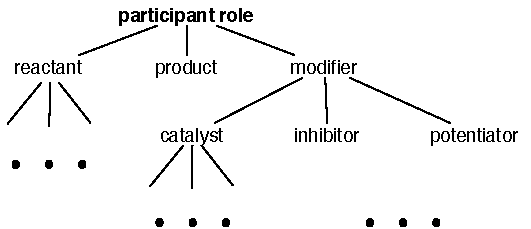
\includegraphics[scale = 0.9]{figs/sbo-participant-role}
  \end{blockMarkChanged}
  \caption{Partial expansion of some of the terms in the
    \emph{participant role} CV of SBO.}
  \label{fig:expanded-species}
\end{figure}

Figure~\ref{fig:expanded-species} shows the anticipated structure
for the \emph{participant role} CV which reflects the hierarchical
conceptual groupings of the concepts. For example, in reaction
rate expressions, there are a variety of possible modifiers.  Some
classes of modifiers can be further subdivided and grouped.  All
of this is easy to capture in the CV.  As more agreement is reached
in the modeling community about how to define and name modifiers
for different cases, the CV can grow to accommodate it.

\begin{figure}[tbh]
  \vspace*{2ex}
  \centering
  \begin{blockMarkChanged}
    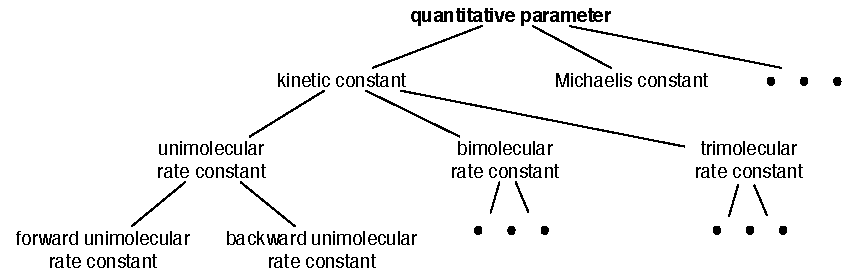
\includegraphics[scale = 0.9]{figs/sbo-quantitative-parameter}
  \end{blockMarkChanged}
  \caption{Partial expansion of some of the terms in the \emph{quantitative
      parameter} CV.}
  \label{fig:expanded-parameter}
\end{figure}

Similar to the above, the controlled vocabulary for quantitative
parameters also has a hierarhical structure, as illustrated in
Figure~\ref{fig:expanded-parameter}.  Note the separation of
\emph{kinetic constant} into separate terms for unimolecular,
bimolecular, etc. reactions, as well as for for forward and
reverse reactions.  The need to have separate terms for forward
and reverse rate constants arises in reversible mass-action
reactions.  This distinction is not always necessary for all
quantitative parameters; for example, there is no comparable
concept for the Michaelis constant.  Another distinction for some
quantitative parameters is a decomposition into different versions
based on the modeling framework being assumed.  For example,
different terms for continuous and discrete formulations of
kinetic constants represent specializations of the constants for
particular simulation frameworks.  Not all quantitative parameters
will need to be distinguished along this dimension.

\begin{wrapfigure}[6]{r}{2.85in}
%\begin{figure}[h]
  \centering
  \vspace*{-2ex}
  \begin{blockMarkChanged}
    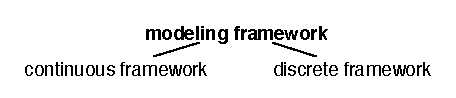
\includegraphics[scale = 0.9]{figs/sbo-framework}
  \end{blockMarkChanged}    
  \vspace*{-2ex}
  \caption{Partial expansion of some of the terms in the
    \emph{modeling framework} CV.}
  \label{fig:expanded-framework}
\end{wrapfigure}
%\end{figure}
The \emph{modeling framework} controlled vocabulary is needed to
support labeling models and reactions with the framework for which
they are designed.  Figure~\ref{fig:expanded-framework}
illustrates the structure of this CV, which is at this point
extremely simple, but we expect that more terms will evolve in the
future.

Finally, there is the \emph{mathematical expression} framework.
This controlled vocabulary encompasses the various mathematical
expressions that constitute a model.
Figure~\ref{fig:sbo-math-expression} illustrates a portion of the
hierarchy.  Rate law formulas are part of the mathematical
expression hierarchy, and subdivided by successively more refined
distinctions until the leaf terms represent precise statements of
common reaction types.  Other types of mathematical expressions
are likely to be included in order to be able to characterize
other mathematical components of a model, namely initial
assignments, assignment rules, rate rules, algebraic rules,
constraints, and event triggers and assignments.

\begin{figure}[tbh]
  \centering
  \begin{blockMarkChanged}
    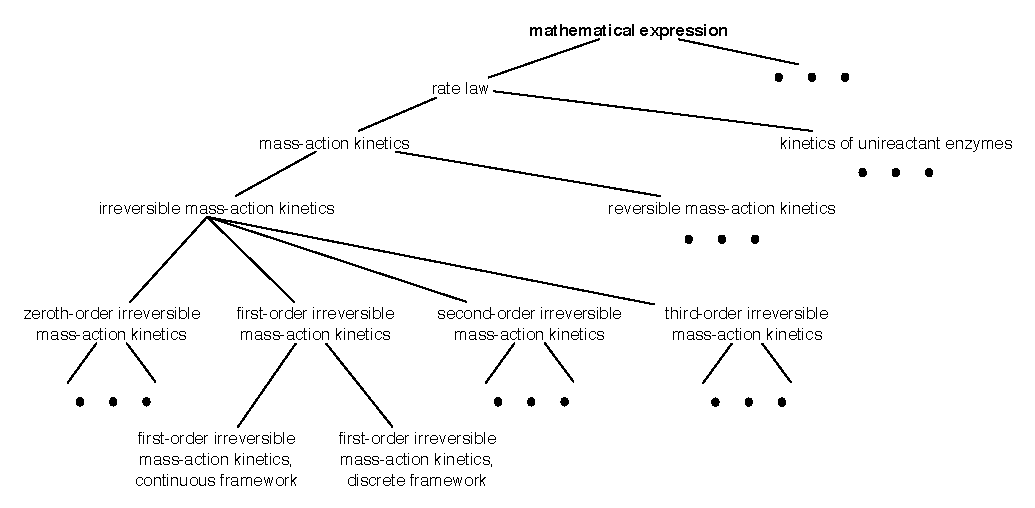
\includegraphics[scale = 0.97]{figs/sbo-math-expression}
  \end{blockMarkChanged}
  \caption{Partial expansion of some of the terms in the \emph{mathematical
      expression} CV.}
  \label{fig:sbo-math-expression}
\end{figure}

The leaf terms of the rate law portion of the SBO mathematical
expression framework contain the mathematical formulas for the
rate laws encoded using \mathmltwo.  There are many potential uses
for this.  One is to allow a software application to obtain the
formula and insert it into a model.  In effect, the formulas given
in the CV act as templates for what to put into an SBML
\KineticLaw definition.  The MathML definition also acts as a
precise statement about the rate law in question.

To make this discussion concrete, here is an example definition of
an entry in the SBO rate law hierarchy at the time of this
writing.  This term represents second-order, irreversible,
mass-action kinetics with one reactant, formulated for use in a
continuous modeling framework:
\begin{quote}
\begin{description}

\item \emph{ID}: \token{SBO:0000052}

\item \emph{Name}: second order irreversible mass action kinetics,
  one reactant, continuous scheme

\item \emph{Definition}: Reaction scheme where the products are
  created from the reactants and the change of a product quantity
  is proportional to the product of reactant activities. The
  reaction scheme does not include any reverse process that
  creates the reactants from the products, and the change of a
  product quantity is proportional to the square of one reactant
  quantity. It is to be used in a reaction modelled using a
  continuous framework.

\item \emph{Parent(s)}: \token{SBO:0000052}, first-order
  irreversible mass-action kinetics (is a)

\item \emph{MathML}:
\begin{example}
<math xmlns="http://www.w3.org/1998/Math/MathML">
   <lambda>
     <bvar><ci definitionURL="http://biomodels.net/SBO/SBO:0000036">k</ci></bvar>
     <bvar><ci definitionURL="http://biomodels.net/SBO/SBO:0000010">R</ci></bvar>
     <apply>
         <times/>
         <ci>k</ci>
         <ci>R</ci>
         <ci>R</ci>
     </apply>
   </lambda>
</math>
\end{example}

\end{description}
\end{quote}

In the MathML definition of the term shown above, the bound
variables in the \token{lambda} expression are tagged with
references to terms in the SBO quantitative parameter (for
\token{k}) and SBO participant role (for \token{R}) vocabularies.
This makes it possible for software applications to interpret the
intended meanings of the parameters in the expression.


%\subsubsection{Interacting with the Systems Biology Ontology}

%We fully anticipate that web service interfaces and software
%libraries will be made available to provide application
%programming interfaces (APIs) to the Systems Biology Ontology,
%allowing software applications to access definitions of SBO terms
%and relationships between them.  The actual SBO ontology is stored
%in a database, but it may be helpful to discuss the content of the
%entries in order to get a sense for the kinds of data fields that
%are likely to be available for each entry in SBO.  The following
%are the minimum anticipated data fields:
%\begin{itemize}\setlength{\parskip}{-0.2ex}
  
%\item \emph{Identifier}: Each term has a unique identifier of type
%  \primtype{SBOType} (Section~\ref{sec:sboterm-type}).

%\item \emph{Name}: Each term is given a name; \eg ``unimolecular
%  rate constant''.
  
%\item \emph{Definition}: Each term includes a written description
%  of its intended meaning.  For example, for ``unimolecular rate
%  constant'', this might be ``Numerical parameter that quantifies
%  the velocity of a chemical reaction involving only one
%  reactant.''
  
%\item \emph{MathML}: For terms that represent final mathematical
%  expressions (\ie the leaf terms of \sbomathformula), the formula
%  is represented using generic \mathmltwo.

%\item \emph{Parents}: The term(s) from which a given term is
%  derived.  The given term has an ``is a'' relationship to its
%  parents.

%\item \emph{Comment}: Additional notable information about the
%  CV term, on an as-needed basis.

%\end{itemize}

%Note that the definitions of formulas, in particular the rate
%laws, are recorded in generic \mathmltwo format.  They
%purposefully do not contain SBML markup.  This permits other,
%non-SBML-aware software applications to use SBO for other
%purposes, and likewise, for other kinds of ontologies to interlink
%with SBO.

One of the goals of SBO is to permit a tool to traverse up and
down the hierarchy in order to find equivalent terms in different
frameworks.  The hope is that when a software tool encounters a
given rate formula in a model, the formula will be a specific form
(say, ``mass-action kinetics, second order, one reactant, for
discrete simulation''), but by virtue of the consistent
organization of the reaction rate CV into framework-specific
definitions, the tool should in principle be able to determine the
definitions for other frameworks (say, ``mass-action kinetics,
second order, one reactant for \emph{continuous} simulation'').
If the software tool is designed for continuous simulation and it
encounters an SBML model with rate laws formulated for discrete
simulation, it could in principle look up the rate laws'
identifiers in the CV and search for alternative definitions
intended for discrete simulation.  And of course, the converse is
true, for when a tool designed for discrete simulation encounters
a model with rate laws formulated for continuous simulation.


\subsubsection{Relationships Between Individual SBML Components and SBO Terms}

The availability of \token{sboTerm} fields on various SBML
components is limited to those for which an SBO label is
appropriate given the goals and principles of SBO's use in SBML
(Section~\ref{sec:sbo-principles}).
Table~\ref{tab:sboterm-availability} summarizes the relationship
between SBML components having \token{sboTerm} fields and the
vocabularies within SBO that apply to that component.

% NOTE: make sure the list in this table matches what's
% defined in \sboelements at the top of this file.

\begin{table}[bht]
  \small
  \centering
  \begin{tabular}{lll}
    \toprule
    \textbf{SBML Component}		& \textbf{SBO Vocabulary} & \textbf{Parent SBO Identifier} \\
    \midrule
    \Model				& modeling framework	  & \sboframeworkID \\
    \Reaction				& modeling framework	  & \sboframeworkID \\
    \Parameter				& quantitative parameter  & \sboparameterID \\
    \SpeciesReference			& participant role	  & \sboparticipantID \\
    \ModifierSpeciesReference		& participant role	  & \sboparticipantID \\
    \KineticLaw				& mathematical expression & \sbomathformulaID \\
    \InitialAssignment			& mathematical expression & \sbomathformulaID \\
    \AlgebraicRule			& mathematical expression & \sbomathformulaID \\
    \AssignmentRule			& mathematical expression & \sbomathformulaID \\
    \RateRule				& mathematical expression & \sbomathformulaID \\
    \Constraint				& mathematical expression & \sbomathformulaID \\
    \Event				& mathematical expression & \sbomathformulaID \\
    \EventAssignment			& mathematical expression & \sbomathformulaID \\
    \bottomrule
  \end{tabular}
  \caption{SBML components and the main types of SBO terms that
  may be assigned to them.  The parent identifiers are provided
  for guidance, but actual annotations should use more specific
  child terms.  See text for explanation.}
  \label{tab:sboterm-availability}
\end{table}

The parent identifiers shown in
Table~\ref{tab:sboterm-availability} are provided for reference.
They are the highest-level terms in their respective vocabularies;
however, these are \emph{not} the terms that would be used to
annotate an element in SBML, because there are more specific terms
underneath the parents shown here.  A software tool should use the
most specific SBO term available for a given concept rather than
using the top-level identifier acting as the root of that
particular vocabulary.

%\subsubsection{Examples}
%\label{sec:sboterm-examples}

%% FIXME

%\textbf{NEED EXAMPLES}


\subsection{Relationships to the SBML \token{annotation} Field}

Another means of providing this kind of information would be to
place it inside the \token{annotation} field
(Sections~\ref{sec:sbase} and~\ref{sec:annotation-standard}).
Although \token{sboTerm} is just another kind of optional
annotation in SBML, the SBO references are separated out and given
a separate field on SBML components, both to simplify their use
for software tools and because they assert a slightly stronger and
more focused connection in a more regimented fashion.  SBO term
references are intended to allow a modeler to make a statement of
the form ``this object is identical to meaning and intention to
the definition of X in the SBO vocabulary'' and do so in a way
that a \emph{software tool can interpret unambiguously}.


\subsubsection{Tradeoffs in Using SBO Terms}

The SBO-based approach to annotating SBML components with
controlled terms has the following strengths:
\begin{enumerate}

\item The syntax is minimally intrusive and maximally simple,
  requiring only one string-valued attribute.

\item It supports a significant fraction of what SBML users have wanted
  to do with controlled vocabularies.

\item It does not interfere with any other scheme.  The more
  general annotation-based approach described in
  Section~\ref{sec:annotation-standard} can still be used
  simultaneously in the same model.

\end{enumerate}

The scheme has the following weaknesses:
\begin{enumerate}

\item An object can only have one \token{sboTerm} field,
  therefore, it can only be related to a single term in SBO.
  (This also impacts the design of SBO: it must be structured such
  that a class of SBML elements can logically only be associated
  with one class of terms in the ontology.)

\item The only relationship that can be expressed by
  \token{sboTerm} is ``is a''.  It is not possible to represent
  different relationships (known as \emph{verbs} in
  ontology-speak).  This limits what can be expressed.

\end{enumerate}

The weaknesses are not shared by the annotation scheme described
in Section~\ref{sec:annotation-standard}.  If an application's
needs cannot be met using SBO terms, software developers should
examine the approach described in
Section~\ref{sec:annotation-standard}.


\subsubsection{When to Use SBO and When to Use Other Annotations}

The general annotation guidelines described in
Section~\ref{sec:annotation-standard} could also be used to make
references to SBO terms.  However, in the interest of making the
use of SBO in SBML maximally interoperable between software tools,
the best-practice recommendation is to place SBO references in the
\token{sboTerm} field rather than in the \token{annotation} field
of an object.

Some software applications may have their own vocabulary of terms
similar in purpose to SBO.  For maximal software interoperability,
the best-practice recommendation in SBML is nonetheless to use SBO
terms in preference to using application-specific annotation
schemes.  Software applications should therefore attempt to
translate their private terms to and from SBO terms when writing
and reading SBML, respectively.


\subsection{Additional Discussion}

Here we discuss some additional points about the SBO-based approach.

\subsubsection{Frequency of Change in the Ontology}
\label{sec:sbo-frequency-of-change}

The SBO development approach follows conventional ontology
development approaches in bioinformatics.  One of the principles
being followed is that identifiers and meanings of terms in the
CVs never change and the terms are never deleted.  Where some
terms are deemed obsolete, the introduction of new terms refine or
supercede existing terms, but the existing identifiers are left in
the CV.  Thus, references never end up pointing to nonexistent
entries.  In the case where synonymous terms are merged after
agreement that multiple terms are identical, the term identifiers
are again left in the CV and they still refer to the same concept
as before.  Out-of-date terms cached or hard-coded by an
application remain usable in all cases.  (Also, with
machine-readable CV encodings and appropriate software design, it
should be possible to develop API libraries that automatically map
older terms to newer terms as the CVs evolve.)

Therefore, a model is never in danger of ending up with SBO
identifiers that cannot be dereferenced.  If an application finds
an old model with a term \token{SBO:0000065}, it can be assured
that it will be able to find this term in SBO, even if it has been
superceded by other, more preferred terms.


\subsubsection{Consistency of Information}

If you have a means of linking (say) a reaction rate formula to a
term in a CV, is it possible to have an inconsistency between the
formula in the SBML model and the one defined for the CV term?
Yes, but this is not a new problem; it arises in other situations
involving SBML models already.  The guideline for these situations
is that the model must be self-contained and stand on its own.
Therefore, in cases where they differ, the definitions in the SBML
model take precedence over the definitions referenced by the CV.
In other words, the model (and its MathML) is authoritative.


\subsubsection{Implications for Network Access}
\label{sec:sbo-implications-for-network-access}

Must a software tool have the ability to access the network or
read the CV every time it encounters a model or otherwise works
with SBML?  No.  Since the SBO will likely stabilize and change
infrequently once a core set of terms is defined, applications can
cache the controlled vocabulary and not make network accesses to
the master SBO copy unless something forces them to (\eg detecting
a reference in a model to an SBO term that the application does
not recognize).  In addition, applications could have user
preference settings indicating how often the CV definitions should
be refreshed (similar to how modern applications provide a setting
dictating how often they should check for new versions of
themselves).  Simple applications may go further and hard code
references to terms in SBO that have reached stability and
community consensus.


\subsubsection{Implications for Software Tools}

What if a software tool does not pay attention to the SBO
annotations described here?  Then one is faced with exactly the
situation that exists today: the SBML model must be interpreted
as-is, without benefit of the information added by the SBO terms.
The purpose of introducing an ontology scheme and guidelines for
its use is to give tools enough information that they \emph{could}
perform added processing, if they were designed to take advantage
of that information.


\subsubsection{Is Another Ontology Really Needed?}

It may seem that developing a new, separate ontology is overkill
for the intended purpose.  However, it turns out that no existing
ontology contains the necessary details for this role in SBML.  In
particular, none of the existing ontologies provide mathematical
formulas for rate laws.


\end{blockChanged}


\begin{blockChanged}
%=============================================================================
\section{A Standard Format for the \token{annotation} Field}
\label{sec:finney-novere}
\label{sec:annotation-standard}
%=============================================================================

This section describes the standard non-proprietary format for
\token{annotation} elements when (a) referring to controlled
vocabulary terms and database identifiers which define and
describe biological and biochemical entities; and (b) describing
the creator of a model and its modification history. Such a
structured format should facilitate the generation of models
compliant with the MIRIAM standard of model
curation~\citep{le_novere:2005}.

This format should \emph{not} be used to refer to SBO terms
(Section~\ref{sec:sboTerm}), because SBO defines terms about
mathematical modelling constructs and not the biological and
biochemical entities that the mathematics represent.

This format uses a restricted form of Dublin
Core~\citep{DCMI:2003} and BioModels qualifier elements (see
\url{http://sbml.org/wiki/Biomodels_Qualifiers}) embedded in
RDF~\citep{w3c:2004}. It uses a number of external XML standards
and associated XML namespaces.
Table~\ref{tab:namespaces-for-standard-annotation} lists these
namespaces and relevant documentation on those namespaces.  The
format constrains the order of elements in these
namespaces beyond the constraints defined in the standard
definitions for those namespaces.  For each standard listed, the
format only uses a subset of the possible syntax defined by the
given standard.  Thus it is possible for an \token{annotation}
element to include XML that is compliant with those external
standards but is not compliant with the format described here.
Parsers wishing to support this format should be aware that a
valid \token{annotation} element may contain an \token{rdf:RDF}
element which is not compliant with the format described here.  A
parser should check that all aspects of the syntax defined here
before assuming that the contained data is encoded in the format.

\begin{table}[bh]
  \begin{blockChanged}
  \small
  \centering
  \begin{tabular}{lll}
    \toprule
    Namespace Prefix & Namespace URI & Definition Document \\
    \midrule
    \token{dc} & \uri{http://purl.org/dc/elements/1.1/} & \citep{powell:2003}\\
    \token{rdf} & \uri{http://www.w3.org/1999/02/22-rdf-syntax-ns\#} & \citep{w3c:2004b} \\
    \token{dcterms} & \uri{http://purl.org/dc/terms/} & \citep{kokkelink:2002}\\
    & & \citep{DCMIUB:2005} \\
    \token{vcard} & \uri{http://www.w3.org/2001/vcard-rdf/3.0\#} & \citep{iannella:2001} \\
    \token {bqbiol} & \uri{http://biomodels.net/biology-qualifiers/} \\
    \token {bqmodel} & \uri{http://biomodels.net/model-qualifiers/} \\
    \bottomrule
  \end{tabular}
  \vspace*{-0.95ex}
  \caption{The XML standards used in the SBML standard format for annotation.
  The namespace prefix are shown to indicate only the prefix used in the main text.}
  \label{tab:namespaces-for-standard-annotation}
  \end{blockChanged}
\end{table}

%=============================================================================
\subsection{General Syntax fo the  standard annotation}
%=============================================================================

An outline of the format syntax is shown below.

\begin{example}
<SBML_ELEMENT +++ metaid="SBML_META_ID" +++ >
  +++
  <annotation>
    +++
    <rdf:RDF
      xmlns:rdf="http://www.w3.org/1999/02/22-rdf-syntax-ns\#"
      xmlns:dc="http://purl.org/dc/elements/1.1/"
      xmlns:dcterm="http://purl.org/dc/terms/"
      xmlns:vcard="http://www.w3.org/2001/vcard-rdf/3.0\#"
      xmlns:bqbiol="http://biomodels.net/biology-qualifiers/" \\
      xmlns:bqmodel="http://biomodels.net/model-qualifiers/" \\
    >
      <rdf:Description rdf:about="#SBML_META_ID">
        [MODEL_HISTORY]
        <RELATION_ELEMENT>
          <rdf:Bag>
            <rdf:li rdf:resource="URI" />
            ...
          </rdf:Bag>
        </RELATION_ELEMENT>
        ...
      </rdf:Description>
      +++
    </rdf:RDF>
    +++
  </annotation>
  +++
</SBML_ELEMENT>
\end{example}

The above outline shows the order of the elements. The capitalized
identifiers refer to generic strings of a particular type:
\texttt{SBML\_ELEMENT} refers to any SBML element name that can
contain an \token{annotation} element; \texttt{SBML\_META\_ID} is
a XML \primtype{ID} string; \texttt{RELATION\_ELEMENT} refers to a
element names in either the namespace
\uri{http://biomodels.net/biology-qualifiers/} or
\uri{http://biomodels.net/model-qualifiers/}; and
\texttt{URI} is a URI.  \texttt{[MODEL\_HISTORY]} refers to an
optional section described in
Section~\ref{sec:model-history-annotation} which can only be
present within SBML model elements. `\texttt{+++}' is a
placeholder for either no content or valid XML syntax that is not
defined by the standard annotation scheme but is consistent with
the relevant standards for the enclosing elements. `\texttt{...}'
is a placeholder for zero or more elements of the same form as the
immediately preceding element.  The precise form of whitespace and
the XML namespace prefix definitions is not constrained.  The rest
of this section describes the format formally in English.

In this format the annotation of an element is located in a single
\token{rdf:RDF} element contained within an SBML
\token{annotation} element. The annotation element can contain
other elements in any order as described in Section \emph{\ref{sec:annotation-use}}.
The format described in this section only defines the form of the
\token{rdf:RDF} element. The containing SBML \SBase element
must have a \token{metaid} field value. (As this attribute is of
the type \primtype{ID} its value must unique to the entire SBML
document.)

The first element of the \token{rdf:RDF} element must be an
\token{rdf:Description} element with an \token{rdf:about}
attribute. (This format doesn't define the form of subsequent
elements of the \token{rdf:RDF} element.) The value of the
\token{rdf:about} attribute must be of the form
\texttt{\#<string>} where the string component is equal to the
value of the \token{metaid} field of the containing SBML element.

The \token{rdf:Description} element can contain only an optional
model history section (see
Section~\ref{sec:model-history-annotation} followed by a sequence
of zero or more BioModels relation elements. The optional model
history section can only be present within an SBML \Model element.
The specific type of the relation elements will vary depending on
the relationship between the SBML component and referenced
information or resource.

Whilst Section~\ref{sec:qualified-dc-annotation} describes the
detailed semantics of each of the relation element types the
content of these elements follows exactly the same form.  The
Biomodels qualifiers relation elements must only contain a single
\token{rdf:Bag} element which in turn must only contain one or
more \token{rdf:li} elements.  The \token{rdf:li} elements must
only have a \token{rdf:resource} attribute containing a URI
referring to an information resource (See
Section~\ref{sec:uri-in-annotation}).

Annotations in this format can be located at different depths
within a model component as is appropriate.

%=============================================================================
\subsection{Use of URIs}
\label{sec:uri-in-annotation}
%=============================================================================

The format represents a set of relationships between the SBML
element and the resources referred to by the contained
\token{rdf:resource} attribute values.  The BioModels relation
elements simply define the type of the relationship.

For instance a \Species element representing a protein
could be annotated with a reference to the database UniProt by the
\uri{http://www.uniprot.org/\#P12999} resource identifier,
identifying exactly the protein described by the \Species
element. This identifier maps to a unique entry in UniProt which
is never deleted from the database. In the case of UniProt, this
is the ``accession'' of the entry. When the entry is merged with
another one, both ``accession'' are conserved. Similarly in a
controlled vocabulary resource, each term is associated with a
perenial identifier. The UniProt entry also possess an ``entry
name'' (the Swiss-Prot ``identifier''), a ``protein name'',
``synonyms'' etc. Only the ``accession'' is perennial and should
be used.

The value of the \texttt{rdf:resource} attribute is a URI that
both uniquely identifies the resource, and the data in the
resource. In this case the resource constraining the identifier
precedes the '\#' symbol and the term or database identifier
follows the '\#' symbol. In the present example, the resource
\uri{http://www.uniprot.org/} includes the entry P12999.

The value of the \texttt{rdf:resource} attribute is a URI, not a
URL; as such, a URI does not have to reference a physical web
object but simply identifies a controlled vocabulary term or
database object (a URI is a label that, in this case, just happens
to look like a URL). For instance, a true URL for an Internet
resource such as \uri{http://www.uniprot.org/entry/P12999} might
correspond to the URI \uri{http://www.uniprot.org/\#P12999}.

SBML does not specify how a parser is to interpret a URI. In the
case of a transformation into a physical URL, there could be
several solutions. For instance, the URI
\uri{http://www.geneontology.org/\#GO:0007268} can be translated
into:

\noindent \uri{http://www.ebi.ac.uk/ego/DisplayGoTerm?selected=GO:0007268}\\
\noindent \uri{http://www.godatabase.org/cgi-bin/amigo/go.cgi?view=details\&query=GO:0007268}\\
\noindent
\uri{http://www.informatics.jax.org/searches/GO.cgi?id=GO:0007268}

Similarly the URI \uri{http://www.ebi.ac.uk/intenz/\#EC 3.5.4.4}
can refer to:

\noindent \uri{http://www.ebi.ac.uk/intenz/query?cmd=SearchEC\&ec=3.5.4.4}\\
\noindent \uri{http://www.expasy.org/cgi-bin/nicezyme.pl?3.5.4.4}\\
\noindent \uri{http://www.chem.qmul.ac.uk/iubmb/enzyme/EC3/5/4/4.html}\\
\noindent \uri{http://www.genome.jp/dbget-bin/www\_bget?ec:3.5.4.4}\\
\noindent etc.

To enable interoperability, the community has agreed on an initial
set of standardized valid URI syntax rules which may be used
within the standard annotation format. This set of rules is not
part of the SBML standard but will grow independently from
specific SBML Levels and Versions. As the set changes a given URI
syntax rule will not be modified although the physical resource
associated with the rule may change. These URIs will always be
composed as \texttt{resource\#id}. The web page
\url{http://sbml.org/wiki/MIRIAM_URI_Set} lists URI syntaxes and
possible physical links to controlled vocabulary and databases.
Each entry contains a list of SBML and relation elements in which
the given URI can be appropriately embedded. To enable consistent
and thus useful links to external resources, the URI syntax rule
set must have a consistent view of the concepts represented by the
different SBML elements for the purposes of this format.  For
example as the rule set is designed to link SBML biological and
biochemical resources the rule set assumes that a \Species element
represents the concept of a biochemical entity type rather than
mathematical symbol. The URI rule list will evolve with the
evolution of databases and resources. The annotation format
described in this section does not require software to access this
list to operate.

%=============================================================================
\subsection{Relation Elements}
\label{sec:qualified-dc-annotation}
%=============================================================================

To enable the format to encode different types of relationships
between SBML elements and resources, different Biomodel qualifier
elements are used to enclose a set of \token{rdf:li} elements. The
relation elements imply a specific relationship between the
enclosing SBML element and the resources referenced by the
\token{rdf:li} elements.

The detailed semantics (i.e. from the perspective of automatic
parser) of the relation elements is defined by the URI list at
\url{http://sbml.org/wiki/MIRIAM_URI_Set}, and thus is outside the
scope of SBML. The URI list generally assumes that the biological
entity represented by the element is the concept linked to the
reference resource.

Several relation elements with a given tag, enclosed in the same SBML
element, each represent an alternative annotation to the SBML
element. For example two \class{bqbiol:hasPart} elements within a
\class{Species} SBML element represent two different sets of
references to the parts making up the the chemical entity
represented by the species. (The species is not made up of all the
entities represented by all the references combined).

The complete list of the qualifier elements in the Biomodels
qualifier namespaces is documented at
\url{http://sbml.org/wiki/Biomodels_Qualifiers}. The list is
divided into two namespaces one for model qualifiers
\uri{http://biomodels.net/biology-qualifiers/} (prefix used here
\token{bqbiol}) and the other for biological qualifiers
\uri{http://biomodels.net/model-qualifiers/}) (prefix used here
\token{bqmodel}.  This list will only grow i.e no element will be
removed from the list. The following is the list of elements at
the time of writing:

%\begin{figure}[htb]
%  \vspace*{2pt}
%  \centering
%\[
%%\begin{CD}
%\textrm{SBML Element}  @>{qualifier}>> \textrm{Referenced Resource} \\
%@VV{represents}V                @VV{represents}V \\
%\textrm{Biological Entity A}   @>{relationship}>>
%\textrm{Biological Entity B}
%%\end{CD}
%\]
%  \caption{How the relationship between biological
%  entities are defined using relations between resources}
%  \label{fig:lenovere-annotation}
%\end{figure}

\begin{itemize}

\item \token{bqmodel:is} The object encoded by the SBML
  component is the subject of the referenced resource. For
  instance, this qualifier should be used to link the model to a
  model database.

\item \token{bqmodel:isDescribedBy} The object encoded by the
SBML component is described by the referenced resource.  This
relation should be used to link SBML components to literature that
describes the component.

\item \token{bqbiol:is} The object encoded by the SBML
  component is the subject of the referenced resource. This
  relation could be used to link a reaction to its exact
  counterpart in KEGG or Reactome for instance.

\item \token{bqbiol:hasPart} The object encoded by the SBML
component includes the subject of the referenced resource, either
physically or logically.

\item \token{bqbiol:isPartOf} The object encoded by the SBML
component is a physical or logical part of the subject of the
referenced resource.

\item \token{bqbiol:isVersionOf} The object encoded by the
SBML component is a version or an instance of the subject of the
referenced resource.

\item \token{bqbiol:hasVersion} The subject of the referenced
resource is a version or an instance of the object encoded by
the SBML component.

\item \token{bqbiol:isHomologTo} The object encoded by the
SBML component is a homolog to the referenced resource.
\end{itemize}

In all cases using the biology qualifiers, the `object' of the
relation is the biological or biochemical object represented by
the enclosing SBML element. In the cases of the model qualifiers,
the `object' of the relation is the model component encoded by the
enclosing SBML element. The resources referenced by the
\class{rdf:li} elements contained within the relation element are
the `object' of the relation.

%===============================================================
\subsection{Model History}
\label{sec:model-history-annotation}
%================================================================

When enclosed in an SBML \Model element, the format described in
previous sections can include additional elements to describe the
history of the model.  This history data must occur immediately
before the first BioModels relation elements.  These additional
elements encode information on the model creator and a sequence of
dates recording changes to the model. The syntax for this section
is outlined below.

\begin{example}
<dc:creator rdf:parseType="Resource">
  <rdf:Bag>
    <rdf:li rdf:parseType="Resource">
      [[
      +++
      <vCard:N rdf:parseType="Resource">
        <vCard:Family>FAMILY_NAME</vCard:Family>
        <vCard:Given>GIVEN_NAME</vCard:Given>
      </vCard:N>
      +++
      [<vCard:EMAIL>EMAIL_ADDRESS</vCard:EMAIL>]
      +++
      [<vCard:ORG>
        <vCard:Orgname>ORGANIZATION_NAME</vCard:Orgname>
      </vCard:ORG>]
      +++
      ]]
    </rdf:li>
    ...
  </rdf:Bag>
</dc:creator>
<dcterms:created rdf:parseType="Resource">
  <dcterms:W3CDTF>DATE<dcterms:W3CDTF>
</dcterms:created>
{<dcterms:modified rdf:parseType="Resource">
  <dcterms:W3CDTF>DATE<dcterms:W3CDTF>
</dcterms:modified>}
\end{example}

The order of elements is as shown above except that elements of
the format contained between \texttt{[[} and \texttt{]]} can occur
in any order.  The capitalized identifiers refer to generic
strings of a particular type: \texttt{FAMILY\_NAME} is the family
name of a person who created the model; \texttt{GIVEN\_NAME} is
the first name of the same person who created the model;
\texttt{EMAIL\_ADDRESS} is the email address of the same person
who created the model; and \texttt{ORGANIZATION\_NAME} is the name
of the organization with which the same person who created the
model is affiliated \texttt{DATE} is a date in W3C date
format~\citep{wolf:1998}. \texttt{W3CDTF}, \texttt{N},
\texttt{ORG} and \texttt{EMAIL} are literal strings. The elements
of the format contained between \texttt{[} and \texttt{]} are
optional. `\texttt{+++}' is a placeholder for either no content or
valid XML syntax that is not defined by the standard annotation
scheme but is consistent with the relevant standards for the
enclosing elements. `\texttt{...}' is a placeholder for zero or
more elements of the same form as the immediately preceding
element. The precise form of whitespace and the XML namespace
prefix definitions is not constrained.  The remaining text in this
section describes the syntax formally in English.

The additional elements of the model history sub-format consist in
sequence of a \token{dc:creator} element, a
\token{dcterms:created} element and zero or more
\token{dcterms:modified} elements.  All these elements must have
the attribute \token{rdf:parseType} set to \texttt{Resource}.

The \token{dc:creator} element describes the person who created
the SBML encoding of the model and contains a single
\token{rdf:Bag} element.  The \token{rdf:Bag} element can contain
any number of elements however the first element must be a
\token{rdf:li} element.  The  \token{rdf:li} element can contain
any number of elements in any order.  The set of elements
contained with the \token{rdf:li} element can include the
following informative elements: \token{vCard:N},
\token{vCard:EMAIL} and \token{vCard:ORG}.  The \token{vCard:N}
contains the name of the creator and must consist of a sequence of
two elements: \token{vCard:Family} and the \token{vCard:Given}
whose content is the family (surname) and given (first) names of
the creator respectively.  The \token{vCard:N} must have the
attribute \token{rdf:parseType} set to \texttt{Resource}.  The
content of the \token{vCard:EMAIL} element must be the email
address of the creator.  The content of the \token{vCard:ORG}
element must contain a single \token{vCard:Orgname} element.  The
\token{vCard:Orgname} element must contain the name of an
organization to which the creator is affiliated.

The \token{dcterms:created} and \token{dcterms:modified} elements
must each contain a single \token{dcterms:W3CDTF} element whose
content is a date in W3C date format~\citep{wolf:1998} which is a
a profile of (restricted form of) ISO 8601.

%================================================================
\subsection{Examples}
%=================================================================

The following shows the annotation of a model with model creation
data and links to external resources:

\begin{example}
<model metaid="_180340" id="GMO" name="Goldbeter1991_MinMitOscil">
    <annotation>
        <rdf:RDF
                xmlns:rdf="http://www.w3.org/1999/02/22-rdf-syntax-ns\#"
                xmlns:dc="http://purl.org/dc/elements/1.1/"
                xmlns:dcterms="http://purl.org/dc/terms/"
                xmlns:vCard="http://www.w3.org/2001/vcard-rdf/3.0\#"
                xmlns:bqbiol="http://biomodels.net/biology-qualifiers/"
                xmlns:bqmodel="http://biomodels.net/model-qualifiers/"
        >
            <rdf:Description rdf:about="#_180340">
                <dc:creator rdf:parseType="Resource">
                    <rdf:Bag>
                        <rdf:li rdf:parseType="Resource">
                            <vCard:N rdf:parseType="Resource">
                                <vCard:Family>Shapiro</vCard:Family>
                                <vCard:Given>Bruce</vCard:Given>
                            </vCard:N>
                            <vCard:EMAIL>bshapiro@jpl.nasa.gov</vCard:EMAIL>
                            <vCard:ORG>
                                <vCard:Orgname>NASA Jet Propulsion Laboratory</vCard:Orgname>
                            </vCard:ORG>
                        </rdf:li>
                    </rdf:Bag>
                </dc:creator>
                <dcterms:created rdf:parseType="Resource">
                    <dcterms:W3CDTF>2005-02-06T23:39:40</dcterms:W3CDTF>
                </dcterms:created>
                <dcterms:modified rdf:parseType="Resource">
                    <dcterms:W3CDTF>2005-09-13T13:24:56</dcterms:W3CDTF>
                </dcterms:modified>
                <bqmodel:is>
                    <rdf:Bag>
                        <rdf:li rdf:resource="http://www.ebi.ac.uk/biomodels/#BIOMD0000000003"/>
                    </rdf:Bag>
                </bqmodel:is>
                <bqmodel:isDescribedBy>
                     <rdf:Bag>
                         <rdf:li rdf:resource="http://www.ncbi.nlm.nih.gov/PubMed/#1833774"/>
                     </rdf:Bag>
                <bqmodel:isDescribedBy>
                <bqbiol:isVersionOf>
                    <rdf:Bag>
                        <rdf:li rdf:resource="http://www.genome.jp/kegg/pathway/#hsa04110"/>
                        <rdf:li rdf:resource="http://www.reactome.org/#69278"/>
                    </rdf:Bag>
                </bqbiol:isVersionOf>
        </rdf:Description>
    </rdf:RDF>
</annotation>
\end{example}

The following example shows a \Reaction structure annotated
with a reference to its exact Reactome counterpart.

\begin{example}
<reaction id="cdc2Phospho" metaid="jb007">
  <annotation>
    <rdf:RDF
      xmlns:bqbiol="http://biomodels.net/biology-qualifiers/"
      xmlns:rdf="http://www.w3.org/1999/02/22-rdf-syntax-ns\#"
    >
      <rdf:Description rdf:about="#jb007">
        <bqbiol:is>
          <rdf:Bag>
            <rdf:li rdf:resource="http://www.reactome.org/\#170156"/>
          </rdf:Bag>
        </bqbiol:is>
      </rdf:Description>
    </rdf:RDF>
  </annotation>
  <listOfReactants>
    <speciesReference species="cdc2"/>
  </listOfReactants>
  <listOfProducts>
    <speciesReference species="cdc2-Y15P"/>
  </listOfProducts>
  <listOfModifiers>
    <modifierSpeciesReference species="wee1"/>
  </listOfModifiers>
</reaction>
\end{example}

The following example describes a species that represents a
complex between the protein calmodulin and calcium ions:

\begin{example}
<species id="Ca_calmodulin" metaid="cacam">
  <annotation>
    <rdf:RDF
      xmlns:rdf="http://www.w3.org/1999/02/22-rdf-syntax-ns\#"
      xmlns:bqbiol="http://biomodels.net/biology-qualifiers/"
    >
      <rdf:Description rdf:about="\#cacam">
        <bqbiol:hasPart>
          <rdf:Bag>
            <rdf:li rdf:resource="http://www.uniprot.org/\#P62158"/>
            <rdf:li rdf:resource="http://www.genome.jp/kegg/compound/\#C00076"/>
          </rdf:Bag>
        </bqbiol:hasPart>
      </rdf:Description>
    </rdf:RDF>
  </annotation>
</species>
\end{example}

The following example describes a species that represents either
``Calcium/calmodulin-dependent protein kinase type II alpha
chain'' or ``Calcium/calmodulin-dependent protein kinase type II
beta chain''. This is the case for instance in the somatic
cytoplasm of striatal medium-size spiny neurons, where both are
present but they cannot be functionally differentiated.

\begin{example}
<species id="calcium_calmodulin" metaid="cacam">
  <annotation>
    <rdf:RDF
      xmlns:rdf="http://www.w3.org/1999/02/22-rdf-syntax-ns\#"
      xmlns:bqbiol="http://biomodels.net/biology-qualifiers/"
    >
      <rdf:Description rdf:about="\#cacam">
        <bqbiol:hasVersion>
          <rdf:Bag>
            <rdf:li rdf:resource="http://www.uniprot.org/\#Q9UQM7"/>
            <rdf:li rdf:resource="http://www.uniprot.org/\#Q13554"/>
          </rdf:Bag>
        </bqbiol:hasVersion>
      </rdf:Description>
    </rdf:RDF>
  </annotation>
</species>
\end{example}

The above approach should not be used to describe ``any
Calcium/calmodulin-dependent protein kinase type II chain''
because such an annotation requires references to the products of
other genes such as gamma or delta. All the known proteins could
be enumerated but such an approach would almost surely lead to
inaccuracies due to the evolution of biological knowledge. Instead
the annotation should refer to a generic information such as
Ensembl family ENSF00000000194 ``CALCIUM/CALMODULIN DEPENDENT
KINASE TYPE II CHAIN'' or PIR superfamily PIRSF000594
``Calcium/calmodulin-dependent protein kinase type II''.

%While with \texttt{HasVersion}, the described component could
%represent several alternative, with \texttt{isVersionOf} the
%described component is one of the alternative understated by the
%referenced resource.

The following two examples show how to use the qualifier
\texttt{is Version Of}. The first example is the relationship
between a reaction and an EC code. An EC code describes an
enzymatic activity and an enzymatic reaction involving a
particular enzyme can be seen as an instance of this activity. For
instance the following reaction represents the phosphorylation of
a glutamate receptor by a complex calcium/calmodulin kinase II.

\begin{example}
<reaction id="NMDAR_phosphorylation" metaid="thx1138">
  <annotation>
    <rdf:RDF
      xmlns:bqbiol="http://biomodels.net/biology-qualifiers/"
      xmlns:rdf="http://www.w3.org/1999/02/22-rdf-syntax-ns\#"
    >
      <rdf:Description rdf:about="#thx1138">
        <bqbiol:isVersionOf>
          <rdf:Bag>
            <rdf:li rdf:resource="http://www.ebi.ac.uk/intenz/\#EC 2.7.1.17"/>
          </rdf:Bag>
        </bqbiol:isVersionOf>
      </rdf:Description>
    </rdf:RDF>
  </annotation>
  <listOfReactants>
    <speciesReference species="NMDAR"/>
  </listOfReactants>
  <listOfProducts>
    <speciesReference species="P-NMDAR"/>
  </listOfProducts>
  <listOfModifiers>
    <modifierSpeciesReference species="CaMKII"/>
  </listOfModifiers>
  <kineticLaw>
    <math xmlns="http://www.w3.org/1998/Math/MathML">
      <apply>
        <times/>
        <ci>CaMKII</ci>
        <ci>kcat</ci>
        <apply>
          <divide/>
          <ci>NMDAR</ci>
          <apply>
            </times>
            <ci>NMDAR</ci>
            <ci>Km</ci>
          </apply>
        </apply>
      </apply>
    </math>
    <listOfParameters>
      <parameter id="kcat" value="1"/>
      <parameter id="Km" value="5e-10"/>
    </listOfParameters>
  </kineticLaw>
</reaction>
\end{example}

The second example of the use of \class{isVersionOf} is the
complex between Calcium/calmodulin-dependent protein kinase type
II alpha chain and Calcium/calmodulin, that is only one of the
``calcium- and calmodulin-dependent protein kinase complexes''
described by the Gene Ontology term GO:0005954.

\begin{example}
<species id="CaCaMKII" metaid="C8H10N4O2">
  <annotation>
    <rdf:RDF
      xmlns:rdf="http://www.w3.org/1999/02/22-rdf-syntax-ns\#"
      xmlns:bqbiol="http://biomodels.net/biology-qualifiers/"
    >
      <rdf:Description rdf:about="\#C8H10N4O2">
        <bqbiol:isVersionOf>
          <rdf:Bag>
            <rdf:li rdf:resource="http://www.geneontology.org/\#GO:0005954"/>
          </rdf:Bag>
        </bqbiol:isVersionOf>
      </rdf:Description>
    </rdf:RDF>
  </annotation>
</species>
\end{example}

The previous case is different form the following one, although they
could seem similar at first sight. The
``Calcium/calmodulin-dependent protein kinase type II alpha
chain'' is a part of the above mentioned ``calcium- and
calmodulin-dependent protein kinase complex''.

\begin{example}
<species id="CaMKIIalpha" metaid="C10H14N2">
  <annotation>
    <rdf:RDF
      xmlns:rdf="http://www.w3.org/1999/02/22-rdf-syntax-ns\#"
      xmlns:bqbiol="http://biomodels.net/biology-qualifiers/"
    >
      <rdf:Description rdf:about="\#C10H14N2">
        <bqbiol:isPartOf>
          <rdf:Bag>
            <rdf:li rdf:resource="http://www.geneontology.org/\#GO:0005954"/>
          </rdf:Bag>
        </bqbiol:isPartOf>
      </rdf:Description>
    </rdf:RDF>
  </annotation>
</species>
\end{example}

It is possible describe a component with several alternative sets of qualified
annotations. For instance, the following species represents a pool
of  GMP, GDP and GDP. We annotate it with the
three corresponding KEGG compound identifiers but also with the
three corresponding ChEBI identifiers.

\begin{example}
<species id="GXP" metaid="GXP">
  <annotation>
    <rdf:RDF
      xmlns:rdf="http://www.w3.org/1999/02/22-rdf-syntax-ns\#"
      xmlns:bqbiol="http://biomodels.net/biology-qualifiers/"
    >
      <rdf:Description rdf:about="\#GXP">
        <bqbiol:hasVersion>
          <rdf:Bag>
            <rdf:li rdf:resource="http://www.ebi.ac.uk/\#CHEBI:17345"/>
            <rdf:li rdf:resource="http://www.ebi.ac.uk/\#CHEBI:17552"/>
            <rdf:li rdf:resource="http://www.ebi.ac.uk/\#CHEBI:17627"/>
          </rdf:Bag>
        </bqbiol:hasVersion>
        <bqbiol:hasVersion>
          <rdf:Bag>
            <rdf:li rdf:resource="http://www.genome.jp/kegg/compound/\#C00035"/>
            <rdf:li rdf:resource="http://www.genome.jp/kegg/compound/\#C00044"/>
            <rdf:li rdf:resource="http://www.genome.jp/kegg/compound/\#C00144"/>
          </rdf:Bag>
        </bqbiol:hasVersion>
      </rdf:Description>
    </rdf:RDF>
  </annotation>
</species>
\end{example}

The following example presents a reaction being actually the
combination of three different elementary molecular reactions. We
annotate it with the three corresponding KEGG reaction, but also
with the three corresponding enzymatic activities.  It is important
to note that the two \class{hasPart} elements represent two
alternative annotations.  The process represented by the
\class{Reaction} structure is composed of three parts, and  not six
parts.

\begin{example}
<reaction id="adenineProd" metaid="adeprod">
  <annotation>
    <rdf:RDF
      xmlns:bqbiol="http://biomodels.net/biology-qualifiers/"
      xmlns:rdf="http://www.w3.org/1999/02/22-rdf-syntax-ns\#"
    >
      <rdf:Description rdf:about="\#adeprod">
        <bqbiol:hasPart>
          <rdf:Bag>
            <rdf:li rdf:resource="http://www.ebi.ac.uk/intenz/\#EC 2.5.1.22"/>
            <rdf:li rdf:resource="http://www.ebi.ac.uk/intenz/\#EC 3.2.2.16"/>
            <rdf:li rdf:resource="http://www.ebi.ac.uk/intenz/\#EC 4.1.1.50"/>
          </rdf:Bag>
        </bqbiol:hasPart>
        <bqbiol:hasPart>
          <rdf:Bag>
            <rdf:li rdf:resource="http://www.genome.jp/kegg/reaction/\#R00178"/>
            <rdf:li rdf:resource="http://www.genome.jp/kegg/reaction/\#R01401"/>
            <rdf:li rdf:resource="http://www.genome.jp/kegg/reaction/\#R02869"/>
          </rdf:Bag>
        </bqbiol:hasPart>
      </rdf:Description>
    </rdf:RDF>
  </annotation>
</reaction>
\end{example}

It is possible to mix different URIs in a given set. The
following example presents two alternative annotations of the human
hemoglobine, the first with ChEBI heme and the second with KEGG
heme.

\begin{example}
<species id="heme" metaid="heme">
  <annotation>
    <rdf:RDF
      xmlns:rdf="http://www.w3.org/1999/02/22-rdf-syntax-ns\#"
      xmlns:bqbiol="http://biomodels.net/biology-qualifiers/"
    >
     <rdf:Description rdf:about="\#heme">
       <bqbiol:hasPart>
         <rdf:Bag>
           <rdf:li rdf:resource="http://www.uniprot.org/\#P69905"/>
           <rdf:li rdf:resource="http://www.uniprot.org/\#P68871"/>
           <rdf:li rdf:resource="http://www.ebi.ac.uk/\#CHEBI:17627">
         </rdf:Bag>
       </bqbiol:hasPart>
       <bqbiol:hasPart>
         <rdf:Bag>
          <rdf:li rdf:resource="http://www.uniprot.org/\#P69905"/>
           <rdf:li rdf:resource="http://www.uniprot.org/\#P68871"/>
           <rdf:li rdf:resource="http://www.genome.jp/kegg/compound/\#C00032"/>
         </rdf:Bag>
       </bqbiol:hasPart>
     </rdf:Description>
   </rdf:RDF>
  </annotation>
</species>
\end{example}

It is possible to mix different qualified sets in the same annotation
element. The following phosphorylation is annotated by its exact
KEGG counterpart and by the generic GO term ``phosphorylation''.

\begin{example}
<reaction id="phosphorylation" metaid="phosphorylation">
  <annotation>
    <rdf:RDF
      xmlns:bqbiol="http://biomodels.net/biology-qualifiers/"
      xmlns:rdf="http://www.w3.org/1999/02/22-rdf-syntax-ns\#"
    >
      <rdf:Description rdf:about="\#phosphorylation">
        <bqbiol:is>
          <rdf:Bag>
            <rdf:li rdf:resource="http://www.genome.jp/kegg/reaction/\#R03313" />
          </rdf:Bag>
        </bqbiol:is>
        <bqbiol:isVersionOf>
          <rdf:Bag>
            <rdf:li rdf:resource="http://www.geneontology.org/\#GO:0016310" />
          </rdf:Bag>
        </bqbiol:isVersionOf>
      </rdf:Description>
    </rdf:RDF>
  </annotation>
</reaction>
\end{example}

\end{blockChanged}


%=============================================================================
\section{Example Models Expressed in XML Using SBML}
\label{sec:xml-rep}
\label{sec:examples}
%=============================================================================

In this section, we present several examples of complete models
encoded in XML using SBML Level~2.

%Our approach to translating
%the UML-based structure definitions presented in the previous
%sections is described elsewhere~\citep{hucka:2000b}.
%Appendix~\ref{apdx:schemas} gives the full listing of an XML
%Schema corresponding to SBML Level~2.


%-----------------------------------------------------------------------------
\subsection{A Simple Example Application of SBML}
\label{sec:modeleg}
%-----------------------------------------------------------------------------

\begin{blockChanged}

Consider the following representation of an enzymatic reaction:
\begin{reaction}\centering\notag
  E + S \eqbm^{\cit k\sub{on}}_{\cit k\sub{off}} ES \yields^{\cit k\sub{cat}} E + P
\end{reaction}
The following is the minimal SBML document encoding the model shown above:

\sbmlexample{enzymekinetics.xml}

In this example, the model has the identifier
\val{EnzymaticReaction}.  The model contains one compartment (with
identifier \val{cytosol}), four species (with identifiers
\val{ES}, \val{P}, \val{S}, and \val{E}), and two reactions
(\val{veq} and \val{vcat}).  The elements in the
\token{<listOfReactants>} and \token{<listOfProducts>} in each
reaction refer to the names of elements listed in the
\token{<listOfSpecies>}.  The correspondences between the various
elements is explicitly stated by the \token{<speciesReference>}
elements.

The model also features local parameter definitions in each
reaction.  In this case, the three parameters (\val{kon},
\val{koff}, \val{kcat}) all have unique identifiers and they could
also have just as easily been declared global parameters in the
model.  Local parameters frequently become more useful in larger
models, where it may become tedious to assign unique identifiers
for all the different parameters.


%-----------------------------------------------------------------------------
\subsection{Example Involving Units}
\label{apdx:units-eg}
%-----------------------------------------------------------------------------

The following model uses the units features of SBML Level~2. In
this model, the default value of \token{substance} is changed
to be mole units with a scale factor
of $-3$, or millimoles.  This sets the default substance units in
the model.  The
\token{size} and \token{time} built-ins are left to their
defaults, meaning size is in litres and time is in seconds.  The
result is that, in this model, kinetic law formulas define rates
in millimoles per second and the species symbols in them represent
concentration values in millimoles per litres.  All the
\token{species} elements set the initial amount of every given
species to 1 millimole.  The parameters \texttt{Vm} and
\texttt{Km} are defined to be in millimoles per litres per second,
and milliMoles per litres, respectively.

\sbmlexample{units.xml}


\end{blockChanged}

%-----------------------------------------------------------------------------
\subsection{Example Involving Assignment Rules}
\label{apdx:rules-eg}
%-----------------------------------------------------------------------------

This section contains a model that simulates a system containing
a fast reaction.  This model uses rules to express the mathematics
of the fast reaction explicitly rather than using the implicit
\token{fast} field on a reaction element.

The system modeled is
\begin{equation*}
  \begin{array}{@{}ccc@{}}
    X_0 & \overset{\underrightarrow{k_1 X_0}}{} & S_1 \\ \\[-4pt]
    S_1 & \overset{\underrightarrow{k_f S_1 - k_r S_2}}{} & S_2 \\ \\[-4pt]
    S_2 & \overset{\underrightarrow{k_2 S_2}}{} & X_1\\ \\[-4pt]
  \end{array}
\end{equation*}
\begin{equation*}
    k_1 = 0.1, \quad k_2 = 0.15, \quad k_f = K_{eq} 10000, \quad k_r = 10000, \quad K_{eq} = 2.5.
\end{equation*}

This can be approximated with the following system:
\begin{equation*}
  \begin{array}{@{}ccc@{}}
    X_0 & \overset{\underrightarrow{k_1 X_0}}{} & T \\ \\[-4pt]
    T & \overset{\underrightarrow{k_2 S_2}}{} & X_1\\ \\[-4pt]
  \end{array}
\end{equation*}
\begin{equation*}
  \begin{array}{ll}
    S_1 = \D\frac{T}{1 + K_{eq}}, & S_2 = K_{eq} S_1\\ \\[-4pt]
  \end{array}
\end{equation*}

The following example SBML model encodes the approximate form.

\begin{blockChanged}
\sbmlexample{assignmentrules.xml}
\end{blockChanged}


%-----------------------------------------------------------------------------
\subsection{Example Involving Algebraic Rules}
\label{sec:algeraiceg}
%-----------------------------------------------------------------------------

This section contains an example model that contains an
\AlgebraicRule structure.  The model contains a different
formulation of the fast reaction described in
Section~\ref{apdx:rules-eg}.

The system described in Section~\ref{apdx:rules-eg} can be
approximated with the following system:

\begin{equation*}
  \begin{array}{@{}ccc@{}}
    X_0 & \overset{\underrightarrow{k_1 X_0}}{} & T \\ \\[-4pt]
    T & \overset{\underrightarrow{k_2 S_1}}{} & X_1\\ \\[-4pt]
  \end{array}
\end{equation*}
\begin{equation*}
  \begin{array}{ll}
    S_2 = K_{eq} S_1\\ \\[-4pt]
  \end{array}
\end{equation*}
with the constraint:
\begin{equation*}
  \begin{array}{ll}
    S_1 + S_2 - T = 0\\ \\[-4pt]
  \end{array}
\end{equation*}

The following example SBML model encodes this approximate form.

\sbmlexample{algebraicrules.xml}


%-----------------------------------------------------------------------------
\subsection{Example with Combinations of
  \token{boundaryCondition} and \token{constant} Values on \class{Species}
  with \class{RateRule} Structures}
\label{sec:constantspecieseg}
%-----------------------------------------------------------------------------

This section contains a model that includes four species each with a
different combination of values of for the \token{boundaryCondition} and
\token{constant} fields.

Consider the following hypothetical system:
\begin{equation*}
  \begin{array}{@{}ccc@{}}
    S_1 + S_2 & \overset{\underrightarrow{k_1 S_1 S_2 S_3}}{} & S_4 \\ \\[-4pt]
  \end{array}
\end{equation*}
$S_3$ is a catalyst that catalyzes the conversion $S_1$ and $S_2$ into $S_4$.
$S_1$ and $S_2$ are on the boundary of the system ($S_1$ and $S_2$ are reactants
but their values are not determined by a kinetic law).
The value of $S_1$ is determined over time by the rate rule:
\begin{equation*}
  \begin{array}{l}
    \D\frac{d S_1}{d t} = k_2 \\ \\[-4pt]
  \end{array}
\end{equation*}
Constant values are:
\begin{equation*}
  \begin{array}{l}
    S_2 = 1 \\ \\
    S_3 = 2 \\ \\
    k_1 = 0.5 \\ \\
    k_2 = 0.1 \\ \\
  \end{array}
\end{equation*}
and initial values are:
\begin{equation*}
  \begin{array}{l}
    S_1 = 0 \\ \\
    S_4 = 0 \\ \\
  \end{array}
\end{equation*}

The value of $S_1$ varies over time so in SBML $S_1$
has a \token{constant} field with a default value of
\val{false}.  The values of $S_2$ and $S_3$ are fixed so in
SBML they have a \token{constant} field values of
\val{true}.  $S_3$ only occurs as a modifier so the value of
its \token{boundaryCondition} field can default to false.  $S_4$ is a
product whose value is determined by a kinetic law and therefore in the
SBML representation has false values, the default values, for both
\token{boundaryCondition} and \token{constant} fields.

The following is the XML document that encodes the model shown
above:

\begin{blockChanged}
\sbmlexample{boundarycondition.xml}
\end{blockChanged}


%-----------------------------------------------------------------------------
\subsection{Example of Translation from a Multi-Compartmental Model to ODEs}
\label{sec:odeeg}
%-----------------------------------------------------------------------------

\begin{blockChanged}

This section contains a model with 2 compartments and 4 reactions.
The model is derived from Lotka-Volterra, with in addition a
reversible transport step.  When instantiated, this model displays
dampened oscillations of three of the species.

\begin{figure}[htb]
  \vspace*{5pt}
  \centering
  \begin{picture}(260,60)
    \put(0,10){\framebox(255,50)[tl]{ cytosol}}
    \put(10,19){\framebox(105,29)[tl]{ nucleus}}
    \put(24,26){$
        X + Y_{1n} \yields^{\cit k\sub{1}} 2\,Y_{1n}
        \eqbm^{\cit K\sub{T}} 2\,Y_{1c} + 2\,Y_2
        \yields^{\cit k\sub{2}} 4\,Y_2 \yields^{\cit k\sub{3}} \emptyset
        $}
  \end{picture}
  \vspace*{-8pt}
  \caption{A example multi-compartmental model.}
  \label{fig:multicomp}
\end{figure}

The model \token{LotkaVolterra\_tranport} is illustrated in
Figure~\ref{fig:multicomp}.  The SBML representation of the model
is shown below, and is followed by its complete translation into
ordinary differential equations.  In this SBML model, the reaction
equations are in substance per time units.  The reactions have
also been simplified to reduce common stoichiometric factors.  The
species variables are in concentration units; their initial
quantities are declared using the attribute \token{initialAmount}
on the \token{species} definitions, but since the attribute
\token{hasOnlySubstanceUnits} is \emph{not} set to true, the
symbols of the species represent their concentrations.  The
species with identifier \val{X} is a boundary condition.  Note the
attribute \token{speciesType}=\val{Y} that tells us species
\val{Y1n} and \val{Y1c} are pools of the same participant, but
located in different compartments.

\sbmlexample{multicomp.xml}

The ODE translation of this model is as follows.  The species
variables in the following equations are all in terms of
concentrations.  First, we give the values of the constant
parameters:
\begin{align*}
  k_1 &= 2500 \\
  k_2 &= 2500 \\
  K_3 &= 25000\\
  K_T &= 2500 \\
\intertext{Initial conditions of variables:}
  V_n & = 1 \\
  V_c & = 5 \\
  X   & = Y1_n = Y2 = 1
\end{align*}

And finally, the differential equations:
\begin{align*}
  \D\frac{d X}{d t}    &= 0 \\[5pt]
  \D\frac{d Y1_n}{d t} &= \D\frac{k_1 \times X \times Y1_n \times V_n - K_T \times (Y1_n - Y1_c) \times V_c}{V_n}
    && \text{reactions production and transport} \\[5pt]
  \D\frac{d Y1_c}{d t} &= \D\frac{K_T \times (Y1_n - Y1_c) \times V_c - k_2 \times Y1_c \times Y2 \times V_c}{V_c}
    && \text{reactions transport and transformation} \\[5pt]
  \D\frac{d Y2}{d t}   &= \D\frac{k_2 \times Y1_c \times Y2 \times V_c - k_3 \times Y2 \times V_c}{V_c}
    && \text{reactions transformation and degradation} \\
\end{align*}

\end{blockChanged}


%-----------------------------------------------------------------------------
\subsection{Example Involving Function Definitions}
\label{sec:functioneg}
%-----------------------------------------------------------------------------

This section contains a model that uses the function definition
feature of SBML.  Consider the following hypothetical system:
\begin{equation*}
  \begin{array}{@{}ccc@{}}
    S_1 & \overset{\underrightarrow{f(S_1)}}{} & S_2 \\ \\[-4pt]
  \end{array}
\end{equation*}
where
\begin{equation*}
  \begin{array}{l}
    f(x) = x * 2 \\ \\[-4pt]
  \end{array}
\end{equation*}

The following is the XML document that encodes the model shown
above:

\sbmlexample{functiondef.xml}


%-----------------------------------------------------------------------------
\subsection{Example Involving \emph{delay} Functions}
\label{sec:delayeg}
%-----------------------------------------------------------------------------

The following is a simple model illustrating the use of $delay$ to
represent a gene that suppresses its own expression.  The model can be
expressed in a single rule:
\begin{equation*}
\frac{d P}{d t} = \D\frac{ \D\frac{1}{1 + m (P_{delayed})^q} - P }{ \tau }
\end{equation*}
where
\begin{equation*}
\begin{array}{rl}
P_{delayed} & \mbox{is } delay(P, \Delta_t) \mbox{ or P at } t - \Delta_t\\
P & \mbox{is protein concentration}\\
\tau & \mbox{is the response time}\\
m & \mbox{is a multiplier or equilibrium constant}\\
q & \mbox{is the Hill coefficient}\\
\end{array}
\end{equation*}

The SBML form of this model is as follows:

\begin{blockChanged}
\sbmlexample{delay.xml}
\end{blockChanged}


%-----------------------------------------------------------------------------
\subsection{Example Involving Events}
\label{sec:eventeg}
%-----------------------------------------------------------------------------

This section presents a simple model system that demonstrates the use of
events in SBML.  Consider a system with two genes, $k_1$ and $k_2$.  $k_1$
is initially on and $k_2$ is initially off.  When turned on, the two genes
lead to the production of two products, $P_1$ and $P_2$, respectively, at a
fixed rate.  When $P_1$ reaches a given concentration, $k_2$ switches off.
This system can be represented mathematically as follows:
\begin{eqnarray*}
  \D\frac{d P_1}{d t} & = & k_1 - P_1\\[3pt]
  \D\frac{d P_2}{d t} & = & k_2 - P_2\\
  k_2 & = &
    \begin{cases}
      0 & \text{when $P_1 \leq \tau$},\\
      1 & \text{when $P_1 > \tau$}.
    \end{cases}
\end{eqnarray*}

The initial values are:
\begin{equation*}
  \begin{array}{lllll}
    k_1 = 1 & k_2 = 0 & \tau = 0.25 & P_1 = 0 & P_2 = 0\\ \\[-4pt]
  \end{array}
\end{equation*}

The SBML Level 2 representation of this as follows:

\sbmlexample{events.xml}


%-----------------------------------------------------------------------------
\subsection{Example Involving Two-Dimensional Compartments}
\label{sec:two-dimensional-eg}
%-----------------------------------------------------------------------------

The following example is a model that uses a two-dimensional compartment.
It is a fragment of a larger model of calcium regulation across the plasma
membrane of a cell.  The model includes a calcium influx channel,
\texttt{Ca\_channel}, and a calcium-extruding PMCA pump, \texttt{Ca\_Pump}.
The model also includes two cytosolic proteins that buffer calcium via the
\texttt{CalciumCalbindin\_gt\_BoundCytosol} and
\texttt{CalciumBuffer\_gt\_BoundCytosol} reactions.

\sbmlexample{twodimensional.xml}


%%-----------------------------------------------------------------------------
%\subsection{Example Using \SpeciesType Structures}
%\label{sec:speciesType-eg}
%%-----------------------------------------------------------------------------

%The following example is a model that uses \SpeciesType structures to indicate
%that 2 pools of biochemical entities (\emph{species}) located in different compartments
%contain the same type of entity (\emph{speciesType}).

%\begin{small}
%\tightspacing
%\begin{verbatim}
%<?xml version="1.0" encoding="UTF-8"?>
%<sbml xmlns="http://www.sbml.org/sbml/level2/version2" level="2" version="2">
%<model id="malate_aspartate_shuttle2">
%    <listOfCompartments>
%        <compartment id="Cytosol"/>
%        <compartment id="Mitochondrial_Matrix"/>
%    </listOfCompartments>
%    <listOfSpeciesTypes>
%        <speciesType id="Aspartate"/>
%    </listOfSpeciesTypes>
%    <listOfSpecies>
%        <species
%            id="Aspartate_in_Cytosol"
%            speciesType="Aspartate"
%            compartment="Cytosol"/>
%        <species
%            id="Aspartate_in_Mitochondrial_Matrix"
%            speciesType="Aspartate"
%            compartment="Mitochondrial_Matrix"/>
%    </listOfSpecies>
%</model>
%</sbml>
%\end{verbatim}
%\end{small}


%=============================================================================
\section{Discussion}
\label{sec:discussion}
%=============================================================================

The volume of data now emerging from molecular biotechnology
leave little doubt that extensive computer-based modeling, simulation and
analysis will be critical to understanding and interpreting the
data~\citep{abbott:1999,gilman:2000,popel:1998,smaglik:2000}.  This
has lead to an explosion in the development of computer tools by many
research groups across the world.  The explosive rate of progress is
exciting, but the rapid growth of the field is accompanied by problems and
pressing needs.

One problem is that simulation models and results often cannot be directly
compared, shared or re-used, because the tools developed by different
groups often are not compatible with each other.  As the field of systems
biology matures, researchers increasingly need to communicate their results
as computational models rather than box-and-arrow diagrams.  They also need
to reuse published and curated models as library components in order to
succeed with large-scale efforts~\cite[e.g., the Alliance for Cellular
Signaling;][]{gilman:2000,smaglik:2000}.  These needs require that models
implemented in one software package be portable to other software packages,
to maximize public understanding and to allow building up libraries of
curated computational models.

We offer SBML to the systems biology community as a suggested format for
exchanging models between simulation/analysis tools.  SBML is an open model
representation language oriented specifically towards representing systems
of biochemical reactions.

Our vision for SBML is to create an open standard that will enable
different software tools to exchange computational models.  SBML is not
static; we continue to develop and experiment with it, and we interact with
other groups who seek to develop similar markup languages.  We plan on
continuing to evolve SBML with the help of the systems biology community to
make SBML increasingly more powerful, flexible and useful.


%=============================================================================
\subsection{Future Enhancements: SBML Level 3 and Beyond}
\label{sec:level-3}
%=============================================================================

As mentioned above, SBML Level 2 is intended to provide a foundation for
modeling biochemical networks.  Many people have expressed a desire to see
additional capabilities added to SBML.  The following summarizes additional
features that are under consideration to be included in SBML Level~3:
\begin{itemize}

\item \emph{Arrays}.  This will enable the creation of arrays of components
  (species, reactions, compartments and submodels).

\item \emph{Connections}.  This will be a mechanism for describing the
  connections between items in an array.

\item \emph{Geometry}.
This will enable the encoding of the spatial characteristics of models
including the geometry of compartments, the diffusion properties of species
and the specification of different species concentrations across different
regions of a cell.

\item \emph{Model Composition}.  This will enable a large model to be built up out
  of instances of other models.  It will also allow the reuse of model
  components and the creation of several instances of the same model.

\item \emph{Multi-state and Complex Species}.  This will allow the straight-forward
    construction of models involving species with a large number of states or
    species composed of subcomponents.  The representation scheme would be designed
    to contain the combinatorial explosion of objects that often results from these
    types of models.

%\item \emph{Controlled Vocabularies}.  This will enable models and model components
%to be labelled with instances of controlled vocabularies.  A model vocabulary
%will describe the SBML features used by a given model.

\item \emph{Diagrams}.  This feature will allow components to be
  annotated with data to enable the display of the model in a diagram.

\item \emph{Dynamic Structure}.  This will enable model structure to vary during simulation.
One aspect of aspect of this allowing
rules and reactions to have their effect conditional on the state of the model system.  For example in
SBML Level 2 it is possible to create a rule with the effect:
\begin{equation*}
\frac{d s}{d t} =
\left\{
\begin{array}{ll}
     0 & \mbox{if $s>0$}\\
     y & \mbox{otherwise}
\end{array}
\right.
\end{equation*}
Dynamic restructuring would enable the expression of the following example:
\begin{equation*}
\begin{array}{ll}
\mbox{if $s>0$} & \D\frac{d s}{d t} = y
\end{array}
\end{equation*}
where $s$ is not determined by the rule when $s \leq 0$.

%\item \emph{Rules for Initial Conditions}.  This will enable the encoding
%  of rules that are only executed at the start of a simulation i.e. set
%  initial conditions.  These rules will be similar to assignment rules and
%  are evaluated in the same sequence as assignment rules but only in the
%  very first instance of simulation.

\item \emph{Tie-breaking algorithm}.  This will include a controlled
  vocabulary and associated fields on models to indicate the
  simultaneous event tie-breaking algorithm required to correctly simulate
  the model.

%\item \emph{Composed Units}.  This will enable a unit definition to be
%composed from one or more other unit definitions.

\end{itemize}


%%=============================================================================
%\subsection{Relationships to Other Efforts}
%\label{sec:other-efforts}
%%=============================================================================

%There are a number of ongoing efforts with similar goals as those of SBML.
%Many of them are oriented more specifically toward describing protein
%sequences, genes and related entities for database storage and search.
%These are generally not intended to be computational models, in the sense
%that they do not describe entities and behavioral rules in such a way that
%a simulation package could ``run'' the models.

%The effort perhaps closest in spirit to SBML is
%CellML\tm~\citep{hedley:2001b}.  CellML is an XML-based markup language
%designed for storing and exchanging computer-based biological models.  It
%includes facilities for representing model structure, mathematics and
%additional information for database storage and search.  Models are
%described in terms of networks of connections between discrete components,
%where a component is a functional unit that may correspond to a physical
%compartment or simply a convenient modeling abstraction.  Components
%contain variables and connections contain mappings between the variables of
%connected components.  CellML provides facilities for grouping components
%and specifying the kinds of relationships that may exist between
%components.  It also uses MathML~\citep{w3c:2000b} for expressing
%mathematical relationships between components and provides the ability to
%use ECMAScript (formerly known as JavaScript) to define functions.

%The constructs in CellML tend to be at a more abstract and general level
%than those in SBML Level~2, and describe the structure and underlying
%mathematics of cellular models in a very general way.  By contrast, SBML is
%closer to the internal object model used in model analysis software.
%Because SBML Level~2 is being developed in the context of interacting with
%a number of existing simulation packages, it is a more concrete language
%than CellML and may be better suited to its purpose of enabling
%interoperability with existing simulation tools.

%The development of SBML Level 2 has benefited from discussions with the
%developers of CellML.  The developers of SBML and CellML are actively
%engaged in ensuring that the two representations can be translated between
%each other.


%%=============================================================================
%\subsection{Tracking the XML Schema Standard}
%\label{sec:tracking-xml}
%%=============================================================================

%One of the problems in attempting to define an XML Schema for SBML is that,
%at the time of this writing, the XML Schema
%specification~\citep{biron:2000,thompson:2000} has not actually been
%finalized.  This has been another motivation for defining SBML in terms of
%abstract data structures in a UML-based notation rather than directly as an
%XML Schema.

%The moving-target status of the XML Schema standard definition requires
%that we plan to update the Schema corresponding to SBML.  The following
%is our planned approach for handling changes in the Schema standard:
%\begin{enumerate}

%\item The definition of SBML Level~2 in this document is
%independent of XML
%  Schema.  Therefore, the definition of SBML Level~2 expressed here can
%  remain the same regardless of what happens to the exact form of XML
%  Schema.  Among other benefits, this allows developers to leave their
%  programs' internal data structures unchanged in the face of possible
%  revisions in the Schema standard.

%%\item In Appendix~\ref{apdx:schemas}, we provide an XML Schema
%%  corresponding to SBML Level~2 that has been created using the current
%%  definition of XML Schema from the W3C
%%  Organization~\citep{biron:2000,thompson:2000}.
%%
%\item Whenever the definition of XML Schema is updated by the W3C in the
%  future, we will issue a revised version of the XML Schema for SBML
%  Level~2 that conform to the updated standard.  We will leave the previous
%  versions still available for reference.  The updated XML Schemas for SBML
%  Level~2 will be identical to the previous versions except where changes
%  in XML Schema force a change in the definition of the Schema for SBML
%  Level~2.

%\end{enumerate}


%=============================================================================
\setcounter{secnumdepth}{-1}
\section{Acknowledgments}
\label{sec:acknowledgements}
%=============================================================================

\begin{blockChanged}
This specification document benefitted from repeated reviews and
feedback by members of the SBML Team, especially Sarah Keating, Bruce
Shapiro, Ben Bornstein, and Maria Schilstra.  We thank them for
their efforts.

The development of SBML was originally funded entirely by the
Japan Science and Technology Agency (JST) under the ERATO Kitano
Symbiotic Systems Project during the years 2000--2003.  The
principal investigators were Hiroaki Kitano and John~C.\ Doyle.
The original SBML Team was lead by Hamid Bolouri and consisted of
Hamid, Andrew Finney, Herbert Sauro, and Michael Hucka.

We gratefully acknowledge sponsorship from many funding agencies.
Support for the continued development of SBML and associated
software, meetings and activities today comes from the following
sources: the National Human Genome Research Institute (USA); grant
number GM070923 from the National Institute of General Medical
Sciences (USA); the International Joint Research Program of NEDO
(Japan); the JST ERATO-SORST Program (Japan); the Japanese
Ministry of Agriculture; the Japanese Ministry of Education,
Culture, Sports, Science and Technology; the BBSRC e-Science
Initiative (UK); the DARPA IPTO Bio-Computation Program (USA); and
the Air Force Office of Scientific Research (USA).  Additional
support has been or continues to be provided by the California
Institute of Technology (USA), the University of Hertfordshire
(UK), the Molecular Sciences Institute (USA), and the Systems
Biology Institute (Japan).

SBML was first conceived at the JST/ERATO-sponsored \emph{First
  Workshop on Software Platforms for Systems Biology}, held in
April, 2000, at the California Institute of Technology in
Pasadena, California, USA.  The participants collectively decided
to begin developing a common XML-based declarative language for
representing models.  A draft version of the Systems Biology
Markup Language was developed by the Caltech ERATO team and
delivered to all collaborators in August, 2000.  This draft
version underwent extensive discussion over mailing lists and then
again during the \emph{Second Workshop on Software Platforms for
  Systems Biology} held in Tokyo, Japan, November 2000.  A revised
version of SBML was issued by the Caltech ERATO team in December,
2000, and after further discussions over mailing lists and in
meetings, we produced a description of SBML
Level~1~\citep{hucka:2001}.  A journal
publication~\citep{hucka:2003} was not produced until much later,
on the occasion of the development of Version~2 of Level~1.

SBML Level~2 was conceived at the \emph{5th Workshop on Software
  Platforms for Systems Biology}, held in July 2002, at the
University of Hertfordshire, UK.  The participants collectively
decided to revise the form of SBML in Level~2.  The first draft of
the Level~2 Version~1 document was released in August 2002. The
final set of features in SBML Level~2 Version~1 was finalized in
May 2003 at the \emph{7th Workshop on Software Platforms for
  Systems Biology} in Ft.\ Lauderdale, Florida.

SBML Level 2 Version~2 was developed with contributions from so
many people constituting the worldwide \emph{SBML Forum} that we
regret it has become infeasible to list individuals by name.  We
are grateful to everyone on the \texttt{sbml-discuss} and
\texttt{libsbml-discuss} mailing lists, the creators of
CellML~\citep{hedley:2001b}, the members of the DARPA Bio-SPICE
project, and the authors of the following software SBML-aware
systems:
BALSA,
BASIS,
BIOCHAM,
BioCharon,
biocyc2SBML,
BioGrid,
BioModels,
BioNetGen,
BioPathway Explorer,
Bio Sketch Pad,
BioSens,
BioSPICE Dashboard,
BioSpreadsheet,
BioTapestry,
BioUML,
BSTLab,
CADLIVE,
CellDesigner,
Cellerator,
CellML2SBML,
Cellware,
CL-SBML,
COPASI,
Cytoscape,
DBsolve,
Dizzy,
E-CELL,
ecellJ,
ESS,
FluxAnalyzer,
Fluxor,
Gepasi,
INSILICO discovery,
JACOBIAN,
Jarnac,
JDesigner,
JigCell,
JWS Online,
Karyote,
KEGG2SBML,
Kinsolver,
libSBML,
MathSBML,
MesoRD,
MetaboLogica,
MetaFluxNet,
MMT2,
Modesto,
Moleculizer,
Monod,
Narrator,
NetBuilder,
Oscill8,
PANTHER Pathway,
PathArt,
PathScout,
PathwayLab,
Pathway Tools,
PathwayBuilder,
PATIKAweb,
PaVESy,
PET,
PNK,
Reactome,
ProcessDB,
PROTON,
pysbml,
PySCeS,
runSBML,
SABIO-RK,
SBML ODE Solver,
SBMLeditor,
SBMLmerge,
SBMLR,
SBMLSim,
SBMLToolbox,
SBliD,
SBToolbox,
SBW,
SCIpath,
Sigmoid,
SigPath,
SigTran,
SIMBA,
SimBiology,
Simpathica,
SimWiz,
SmartCell,
SRS Pathway Editor,
StochSim,
STOCKS,
TERANODE Suite,
Trelis,
Virtual Cell,
WinSCAMP,
and
XPPAUT.


\end{blockChanged}

%BASIS, BioSketchPad, BioSpice, CellDesigner, Cellerator, CellML,
%COPASI, DBSolve, E-Cell, ESS, Gepasi, Jarnac, JDesigner, JigCell, MCell,
%NetBuilder, Promot/DIVA, StochSim, and Virtual Cell, and members of the
%\texttt{sysbio} and \texttt{sbml-discuss} mailing lists.  We are
%particularly grateful to the following people for discussions, advice and
%comments: Nicolas Allen, Adam Arkin, Hamid Bolouri, Ben Bornstein, Dennis
%Bray, Roger Brent, Steve Burbeck, Claudine Chaouiya, Kwang Cho, Athel
%Cornish-Bowden, Manuel Corpas, Autumn Cuellar, John Doyle, Serge Dronov,
%Drew Endy, David Fell, Carl Firth, Ed Frank, Akira Funahashi, Ralph Gauges,
%Martin Ginkel, Victoria Gor, Igor Goryanin, Warren Hedley, Charles Hodgman,
%Stefan Hoops, Nick Juty, Jay Kaserger, Sarah Keating, Hiroaki Kitano, Ben
%Kovitz, Andreas Kremling, Nicolas Le~Nov\`{e}re, Fred Livingston, Les Loew,
%Daniel Lucio, Joanne Matthews, Mike McCollum, Pedro Mendes, Eric Minch,
%Eric Mjolsness, David Morley, Mineo Morohashi, Poul Nielsen, Greg Peterson,
%Mark Poolman, Carole Proctor, Wayne Rindone, Sven Sahle, Takeshi Sakurada,
%Vijay Saraswat, Herbert Sauro, James Schaff, Maria Schilstra, John Schwacke,
%Cliff Shaffer, Bruce Shapiro, Tom Shimizu, Herbert Sauro, Hugh Spence,
%J\"{o}rg Stelling, Kouichi Takahashi, Masaru Tomita, Marc Vass, John Wagner,
%Jonathan Webb, J\"{o}rg Weimar, Darren Wilkinson, Olaf Wolkenhauer and Tau-Mu Yi.


%\changed{Both versions of SBML Level 2 were} created in
%collaboration with the authors of the following systems:
%\emph{BASIS}~\citep{kirkwood:2003},
%\emph{Bio Skektch Pad}~\citep{belta:2003},
%\emph{BioSpreadsheet}~\citep{mccollum_2003},
%\emph{BioSpice}~\citep{arkin:2001},
%\emph{CellDesigner}~\citep{funahashi:2003},
%\emph{Cellerator}~\citep{shapiro:2001,shapiro:2003b},
%\emph{COPASI}~\citep{mendes:2000},
%\emph{DBsolve}~\citep{goryanin:2001,goryanin:1999},
%\emph{E-CELL}~\citep{tomita:1999,tomita:2001},
%\emph{ESS}~\citep{peterson:2003},
%\emph{Gepasi}~\citep{mendes:1997,mendes:2001},
%\emph{Jarnac}~\citep{sauro:2000,sauro:1991},
%\emph{JDesigner}~\citep{sauro:2001b},
%\emph{JigCell}~\citep{vass:2003},
%\emph{MCell}~\citep{bartol:2002},
%\emph{NetBuilder}~\citep{schilstra:2002},
%\emph{PathScout}~\citep{minch_2003},
%\emph{ProMoT/DIVA}~\citep{stelling:2001},
%\emph{StochSim}~\citep{bray:2001,morton-firth:1998}, and
%\emph{Virtual Cell}~\citep{schaff:2000,schaff:2001}.
%\changed{Both versions of SBML Level 2 were} developed with the help of these
%packages' authors, as well as help and collaboration from the
%creators of CellML~\citep{hedley:2001b} and many other individuals
%listed in the Acknowledgments
%(Section~\ref{sec:acknowledgements}).



\newpage
\setcounter{secnumdepth}{2}
\appendix

%-----------------------------------------------------------------------------
\section{\changed{Differences between SBML Level 1 Version 2 and Level 2 Version 1}}
%-----------------------------------------------------------------------------
\label{apdx:level1-level2}

\changed{Compared to SBML Level 1 Version 2, SBML Level 2 Version
1 introduces the following changes:}
\begin{itemize}

\item SBML Level 2 supports the inclusion of metadata using the same approach as
  CellML~\citep{cuellar:2002}.  All structures in SBML can be annotated
  with optional content in RDF~\cite[Resource Description
  Format;][]{lassila:1999} following the guidelines put forward by
  \citeauthor{cuellar:2002}. (Section~\ref{sec:sbase}.)

\item All data structures, including \Sbml and
  \token{listOf}\rule{0.5in}{0.5pt} elements, are now derived from the type
  \SBase.  (Section~\ref{sec:sbase}.)  This means all major
  structures in SBML can have separate annotations and metadata associated
  with them.

\item A new field, \token{id}, replaces the \token{name} field previously
  defined for most SBML structures to identify each part of a model.  (See
  Section~\ref{sec:idnameattribs}.)  The \token{id} field has a type of
  \primtype{SId}, whose definition is similar to \token{SName} in Level~1.  In
  SBML Level~2, the \token{name} field is optional and is defined to allow
  any Unicode characters allowed by the \primtype{string} type of XML
  Schema~\citep{biron:2000}.

\item Formulas in Level~2 are expressed using MathML~\citep{w3c:2000b} 2.0.
  The field named \token{formula} previously available on the
  \KineticLaw and \Rule structures has been replaced by a
  MathML element named \token{math} containing MathML content.  In
  addition, stoichiometry numbers may now be expressed using MathML,
  allowing for more flexibility in defining reactions.
  (Sections~\ref{sec:formulas}, \ref{sec:rules} and~\ref{sec:reactions}.)

\item The namespace for identifiers in a model does not contain any
  built-in symbols; gone, for example, are the predefined rate laws of SBML
  Level~1.  The approach taken in SBML Level~2 is that each model must
  itself define whatever functions it needs using the new
  \FunctionDefinition mechanism.  Although SBML Level~2 \emph{does}
  define two built-in entities (a symbol representing time and another
  symbol representing delay functions), these are referenced using a
  feature of MathML and are not in the same namespace as identifiers
  defined by a model.  (Section~\ref{sec:csymbol-token}.)

\item SBML Level~2 makes explicit a previously unstated assumption, that
  the XML encoding of a model uses UTF-8.  SBML documents must refer to the
  UTF-8 encoding in their XML declaration.  (Section~\ref{sec:sbml}.)

\item The top-level \Model structure can contain an optional list of
  global user-defined functions expressed in MathML and organized in new
  structures of type \FunctionDefinition.  (Sections~\ref{sec:model}
  and \ref{sec:functiondefinition}.)

\item The top-level \Model structure can contain an optional list of
  event definitions organized in structures of type \Event.  Events
  define discrete changes in model behavior at specific times during a time
  simulation of the model.  (Section~\ref{sec:model} and \ref{sec:events}.)

\item Unlike in SBML Level~1, unit identifiers in Level~2 are in a separate
  namespace from the namespace used for models, functions, species,
  compartments, reactions and parameters.  Also, the unit names
  ``\token{meter}'' and ``\token{liter}'' are not defined in Level~2 because
  the SBML user community deemed them unnecessary.  Finally, \Unit
  structures now have the additional fields \token{multiplier} and
  \token{offset} to enable the definition of non-SI units.
  (Section~\ref{sec:unitdefinitions}.)

\item The \Compartment structure has a new field,
  \token{spatialDimensions}, whose value is a positive integer specifying
  the number of dimensions in space the compartment possesses.  This
  enables the definition of such things as two-dimensional membranes.  As a
  side-effect, the units of species concentration in SBML Level~2 depend on
  the spatial dimensions of the compartment where the species is located.
  To support these new capabilities, \token{Compartment} now uses a field
  named \token{size} instead of \token{volume}, and there are two new
  built-in units for area and length.  (Sections~\ref{sec:unitdefinitions}
  and \ref{sec:compartments}.)

\item All fields representing initial conditions or parameter values,
  including compartment sizes and species concentrations, are optional in
  Level~2.  A missing value for one of these fields implies that the value
  is either unknown, not required for analysis, or should be obtained from
  an external source. (Sections~\ref{sec:compartments}, \ref{sec:species}
  and \ref{sec:parameters}.)

\item The \Compartment, \Species and \Parameter
  structures each have a new boolean field named \token{constant}.  This
  field specifies whether the variables represented by these structures can
  be changed by rules and reactions.  (Sections~\ref{sec:compartments},
  \ref{sec:species} and~\ref{sec:parameters}.)

\item The \Species structure has a new field,
  \token{initialConcentration}, for setting the initial value of a species
  in terms of its concentration.  This is in addition to the ability,
  carried over from Level~1, to set the values in terms of amounts.
  (Section~\ref{sec:species}.)

\item The \Species structure has two new fields, \token{spatialSizeUnits}
  and \token{substanceUnits}, which replace the \token{units} field in Level~1.
  These fields are composed to form the concentration units of the species
  symbol.  (Section~\ref{sec:species}.)

\item The rule structures are simpler compared to SBML Level~1.
\changed{There is
  no longer a \token{type} field on \AssignmentRule.  A redesigned structure
  \AssignmentRule and new \RateRule structure replace SBML Level~1's
  \token{ParameterRule}, \token{SpeciesConcentrationRule} and
  \token{CompartmentVolumeRule}.}  (Section~\ref{sec:rules}.)

\item The \Reaction structure has a new list of \emph{modifiers} in
  addition to the list of reactants and products.  The
  \token{listOfModifiers} enumerates species that affect a reaction but
  are neither created nor destroyed by the reaction.
  (Section~\ref{sec:reactions}.)

\end{itemize}

\begin{blockChanged}
%-----------------------------------------------------------------------------
\section{Differences between SBML Level 2 Version 1 and Level 2 Version 2}
\label{apdx:version1-version2}
%-----------------------------------------------------------------------------

The changes introduced by \sbmltwotwo over \sbmltwoone as
described by this specification are divided into 2 parts: (a) new
and changed features and, (b) Version~1 errata corrected in
Version~2.

\subsection{Feature Changes Relative to \twoone}

The features introduced or changed in Version 2 are:
\begin{itemize}
  
\item \emph{XML namespace}.  Version 2 uses the XML namespace
  \uri{http://www.sbml.org/sbml/level2/version2}.
  
\item \emph{Removal of predefined annotation namespaces}.  In
  Section~\ref{sec:annotation-use}, previous Levels and Versions
  of SBML reserved a set of XML Namespace names corresponding to
  software tools known to exist at the time.  Due to the explosion
  of SBML-compatible software tools in recent years, it has become
  infeasible to maintain such a list; moreover, informal
  discussions with SBML users revealed that no one paid much
  attention to the list anyway.  Beginning with SBML Level~2
  Version~2, no such namespaces are defined in the SBML
  specification.
  
\item \emph{One top level element per XML Namespace per
    \token{annotation} element and associated restrictions}.  An
  \token{annotation} element cannot contain two or more top level
  elements in the same XML namespace.  An \token{annotation}
  element cannot contain a top level element in the SBML
  namespace.  The order of top level elements within an
  \token{annotation} element is not significant.
  
\item \emph{Introduction of \token{sboTerm}}.  In Version 2, the
  \sboelements structures have an addition field named
  \token{sboTerm}.  This field is of type \primtype{SBOTerm}.  Its
  value is permitted to be only valid Systems Biology Ontology
  (SBO) identifiers.  (Section~\ref{sec:sboTerm}.)
  
\item \emph{New format for linking external resources to SBML}.  A
  new format for using RDF and Dublin Core within
  \token{annotation} elements to link SBML models to external
  resources and record model version history is introduced. Whilst
  CellML metadata can be included in SBML the specification does
  not make any specific mention of CellML metadata.
  
\item \emph{Built-in units can be dimensionless}.  In \twotwo, the
  built-in units (\eg \token{substance}, \token{volume} and
  others), can be assigned \token{dimensionless} units. This
  facilities the correct encoding of models based on dimensionless
  experimental data.
  
\item \emph{\Unit no longer has an \token{offset}
    field}.  In Version 2, the \token{offset} field on
  \Unit has been removed because it was impossible to
  define consistently with the rest of the SBML unit system.
  Either a complicated set of special exceptions and rules would
  have had to be introduced to enable proper interpretation of
  units with offsets, or the offset field could be removed.  Since
  the situations requiring offsets are so infrequent, removing the
  offsets was judged to be the lesser of evils.  As a benefit, the
  unit system of \sbmltwotwo is streamlined and straightforward to
  implement, which may encourage more software developers to
  support it.

%\item \emph{Substance units can be mass derived}

%In Version 2 the \emph{substance} built-in unit can be derived
%directly from kilogram rather from mole.  This facilitates the
%correct encoding of models that use a mass based rather mole based
%units system (see \citep{domach:2000, castellanos:2004} for
%examples of such models).
  
\item \emph{Compartment Type}. In Version 2 the \Model structure
  has an addition list of \CompartmentType structures.  Each of
  these structures represents a type of compartment and consists
  of just \token{name} and \token{id} fields.  The \token{id}
  field can optionally be referenced from an \Compartment
  structure using a new \token{compartmentType} field.
  
\item \emph{Species Type}.  In Version 2 the \Model structure has
  an addition list of \SpeciesType structures.  A \SpeciesType
  structure represents a type of chemical entity independent of
  location and consists of just \token{name} and \token{id}
  fields.  The \token{id} field can optionally be referenced from
  an \Species structure using a new \token{speciesType} field.
  
\item \emph{\token{charge} field deprecated}.  In Version 2 the
  \Species structure \token{charge} field is deprecated.
  
\item \emph{Constraints}.  In Version 2, the \Model structure has
  an addition list of \Constraint structures.  The \token{math}
  field of \Constraint contains a boolean expression which is is
  function of the model state which returns whether the state is
  valid.  Unlike the \Rule structures \Constraint should not be
  used to compute the dynamical behavior of the model.
  
\item \emph{\token{Id} on \SimpleSpeciesReference}.  Version 2
  adds \token{id} and \token{name} fields to the
  \SimpleSpeciesReference structure.  The \token{id} field
  declares an identifier which is in the global namespace of
  objects.
  
\item \emph{Reaction identifier as a symbol in math expressions}.
  In Version 2 the value of the \token{id} of any reaction can
  appear in an expression within a MathML \token{ci} element.  The
  symbol represents the rate of the reaction which is given by the
  \KineticLaw structure of the \Reaction.  It is not possible to
  explicitly assign a value to the symbol using
  \InitialAssignment, \EventAssignment, \AssignmentRule or
  \RateRule structures.
  
\item \emph{Initial Assignment Structures}.  In Version 2 the
  \Model structure has an additional list of \InitialAssignment
  structures.  This list of structures is evaluated before an
  reactions or other rules to determine the values of constants
  and the initial values of variables.  Assignment rules override
  the values calculated by the \InitialAssignment structures.
  
\item \emph{The order of \AssignmentRule structures is not
    significant}.  In Version 2 the order of \AssignmentRule is
  not significant however the set of assignment rules formed from
  \KineticLaw, \InitialAssignment and \AssignmentRule structures
  as a whole must not contain algebraic loops.

\item \emph{Strong interpretation of \token{fast} on \Reaction}
  
  Until \twotwo, it was assumed that the \token{fast} field on
  \Reaction could be ignored by software tools that did not have
  the capacity to support it.  Further research has shown that
  this is not true.  \sbmltwotwo stipulates that if a model has
  values for \token{fast}, a software tool must be able to respect
  the field or else indicate to the user that it does not have the
  capacity to do so.
  
\end{itemize}


\subsection{Incorporation of errata from \sbmltwoone}

The errata in the SBML Level 2 Version 1 specification that
corrected in this Version 2 specification are as follows.  The
page and section numbers refer to the final PDF version of the
SBML Level 2 Version 1 specification.

\begin{itemize}

\item page 1: The specification should contain a link to the
latest version of the specification and to this specific
\emph{issue} of the document.

\item page 2: Each additional errata to the specification should
result in an new issue of the specification each with a unique
number.  The first issue of the specification should be numbered
1.  The errata on this specification should recorded in a new
section starting in issue 2.  Each errata will be numbered with
the issue in which the errata is introduced.  Errata should not
change the fundamental semantics or syntax of SBML but merely
clarify and disambiguate the specification.

%\item page 2: Each new level, version and issue of SBML should be
%announced on a low volume emailing list mentioned in the
%specification.

\item page 2: The specification should make explicit the features
which are not backwards compatable between Level 2 Version 2 and
Level 2 Version 1.

\item page 3 Section 1.2: The specification should make explicit
the differences in the numeric types of XML Schema and MathML.

\item page 4 Section 3.1: This section should include an
explanation of why \token{id} and \token{name} fields are not
present on \SBase.

\item page 8 Figure 3: Change \texttt{nameChar} and \texttt{name}
to \texttt{idChar} and \texttt{SId} to indicate clearly the use of
the BNF syntax definition.

\item page 9 Section 3.6: The specification should reference
existing documents to clarify the semantics of the MathML
operators in the MathML subset.

\item page 9 Section 3.6: The specification should constrain the
use of MathML operators which return different types of result
(numeric or boolean) appropriately.

\item page 9 Section 3.6.1: The \token{encoding} attribute is
permitted on \token{annotation} and
\token{annotation-xml} elements in MathML, not only on
\token{csymbol} as stated on that page.

\item page 9 Section 3.6.1: The \mathmltwo standard specifies the
result of n-ary operators when the number of operands is
critically small, for example for \token{times} and \token{add}
elements, when the number of operands are zero or one.  This is an
obscure part of MathML and the specification should highlight the
relevant sections of the MathML specification.

\item page 9 Section 3.6.2: The specification should make explicit
the differences in the numeric types of XML Schema and MathML.

\item page 9 Section 3.6.2: The specification should describe the
MathML whitespace rules for \token{cn} elements.

\item page 10 Section 3.6.3: The specification should describe the
MathML whitespace rules for \token{ci} elements.

\item page 10 Section 3.6.3: The specification should state
whether SBML has early or late binding semantics.

\item page 10, Section 3.6.4: The delay function is not clearly
defined. There is no explanation of what range of values is valid
for the time.  For example, can delay times be less than zero?
Also, are there restrictions on the acceptable values of the
argument $x$?

\item page 13, Section 4.3.1: The `can' in the second sentence
should be replaced by `should'.

\item page 14, Section 4.4.2: The \token{id} field of a
\UnitDefinition structure must not contain a value from
Table 2, the table of \primtype{UnitKind} values.  This restriction
is necessary because otherwise a unit definition could redefine
one of the base unit kinds.

\item page 14, Section 4.4.2: The first formula should be the
following:
\begin{equation*}
u_{new} = (\emph{multiplier} \times 10^{\emph{scale}} \times
u)^{\emph{exponent}} + \emph{offset}
\end{equation*}  This equation is superseded by modifications
to the \Unit and \UnitDefinition structures in this specification
\sbmltwotwo.

\item page 16, Section 4.4.3: The example code redefining the
built-in unit \texttt{volume} should replace \texttt{liters} with
\texttt{litre}. \texttt{liters} is not a valid value for the
\token{kind} attribute.

%\item page 17 Section 4.5.5 and page 19 Section 4.6.4: The text is
%slightly contradictory.  The text needs to be improved.

\item page 18 section 4.5.6: the value of \token{outside} field
for a given \Compartment structure must be the value of an
\token{id} field of another \Compartment structure.

\item page 18 Section 4.5.6: The graph formed where compartments
are nodes and the arcs are implied by the values of
\token{outside} attributes must be acyclic otherwise a
compartment can be outside itself.

\item page 19 Section 4.6.3: On \Species elements the
\token{initialConcentration} attribute can have a value even if
the \token{hasOnlySubstanceUnits} attribute is ``\texttt{true}''.

\item page 19 Section 4.6.4: This section should contain a table
that shows how the units of a species is determined from the
spatial dimensions of the species and the value of the
\token{hasOnlySubstanceUnits} attribute.

\item page 24 Section 4.8.4: This section should specify that the
model should not be overdetermined as defined in
Section~\ref{sec:ruleconstraints} of the SBML Level 2 Version 2
specification (i.e. this document).

\item page 24 Section 4.8.4: This section should not refer to
assignment rules using the term `scalar rule'.

\item page 27 Section 4.9.5: If a species id occurs in any
\token{ci} element MathML element including \KineticLaw and
\StoichiometryMath elements it should appear in a
\SimpleSpeciesReference element in the reaction.  The
specification only applies this rule to the \KineticLaw
element. Such a species is at a minimum a modifier of the
reaction.

\item page 29 Section 4.9.5: The relationship of the abstract
class \SimpleSpeciesReference to the concrete classes
\SpeciesReference and \ModifierSpeciesReference
should be made explicit.

\item page 29 Section 4.9.6: Despite being redundant it is
possible for a species to be referenced from the \token{modifier}
field whilst being referenced from the \token{product} and/or
\token{reactant} fields of the same reaction.

\item page 29 section 4.9.7: 3rd paragraph: The text is overly
restrictive and contradictory with respect of the units of species
symbols. Species symbols can be either amount or concentration
units depending on the species declaration.

\item page 29 section 4.9.7: Final paragraph: The kinetic law
expression is composed so that the units are of the parameter are
not those conventionally used.  This is not good practice.  The
rate law expression should be changed to include the compartment
volume so that the units of the parameter are those that would be
measured by an experimentalist and used in practice by a modeler.

\item page 31 Section 4.10.5: A \token{variable} attribute on a
\EventAssignment element should be unique among the set of
assignments within an \Event element if not the effect of
event assignment is ambiguous.

\item page 31 Section 4.10.5: A \token{variable} attribute on a
\EventAssignment element should not have the same value as
a \token{variable} attribute on a \AssignmentRule element.

\item page 32 Section 4.10.7: \emph{Any} transition of a
\token{trigger} expression from false to true will cause an
\token{event} to \emph{fire}.  Consider an \token{event} $E$ with
delay $d$ where the \token{trigger} expression makes a transition
from false to true at times $t_1$ and $t_2$.  The
\EventAssignment structure will have effect at $t_1+d$ and
$t_2+d$ irrespective of the relative times of $t_1$ and $t_2$. For
example events can ``overlap'' so that $t_1 < t_2 < t_1+d$ still
causes event assignments to occur at $t_1+d$ and $t_2+d$.

\item page 32 Section 4.10.7: Events cannot be triggered at $t=0$.

\item page 34 Section 5.2: The units of parameter \texttt{Km}
should be moles per litre as the parameter is added to the
concentration of a species.

\item page 38 Example 5.3: The \texttt{out} reaction should have a
\token{listOfModifiers} which refers to species \texttt{S2} since
it is referenced in the reaction's \KineticLaw.

\item page 40 Example 5.5: The one rule in \token{listOfRules}
should not use \texttt{<apply> ... </apply>}; these tags should be
omitted.

\item page 42 Example 5.6: The MathML in the two \RateRule
definitions should not use \texttt{<apply> ... </apply>}; these
tags should be omitted.

\item page 46 Example 5.8: The value of the \token{definitionURL}
attribute on a \token{csymbol} delay should be
\texttt{http://www.sbml.org/sbml/symbols/delay}, not
\texttt{http://www.sbml.org/symbols/delay} (the incorrect form
omitted ``\texttt{sbml}'').

\item page 55 Appendix A: The appendix states that UML inheritance
is mapped, in XML Schema, to the \texttt{extension} of
\token{complexType} elements. This is by far the most natural
interpretation and the one used in the schema available on the
SBML web site and used by libSBML. However, this approach
introduced a restriction: an ordering of elements is imposed on
all extended types because the definition of XML Schema
effectively requires the use of \texttt{sequence} ordering in
order to be able to use type inheritance in this way. (A full
explanation of the details can be found in Section 13.5 of
~\cite{walmsley:2002} ) The result is that the ordering of
subelements in SBML XML is important.  For example, \token{notes}
and \token{annotation} elements must occur before
\token{listOfReactants} elements within a \Reaction
element. Appendix A should state this restriction explicitly.
Appendix A should be moved into the main text.  The dependence on
\texttt{sequence} is a result of using XML Schema.

\item page 55 Appendix A: The SCHUCS document doesn't state what
model group element should be used in the XML schema
interpretation of UML. (Examples of XML schema are that
\token{xs:element} elements should be enclosed in
\token{xs:choice}, \token{xs:all} or \token{xs:sequence} elements;
see p.488 table A-1 of~\cite{walmsley:2002}.) To be consistent
with the previous errata item, \token{xs:sequence} elements should
be used.  (The SBML schemas use this interpretation).

\item page 56, Appendix B: The last bullet, second sentence
starts: ``there is no longer a \token{type} field on
\Rule''. Technically, this should read: ``there is no
longer a \token{type} field on \AssignmentRule''.

\end{itemize}


\end{blockChanged}
%=============================================================================
\section{XML Schema for SBML}
\label{apdx:schema}
%=============================================================================

The following is an XML Schema definition for the SBML Level 2
Version 1, using the W3C Recommendation for XML Schema version 1.0
of 2 May 2001~\citep{biron:2000,fallside:2000,thompson:2000}. This
schema does not define all aspects of SBML Level 2: a SBML
document validated by this schema is not necessarily a valid SBML
Level 2 document.  Appendix~\ref{apdx:mathml-subset-schema}
contains a a schema for the SBML MathML subset.
Appendix~\ref{apdx:validation-rules} contains a list of the
remaining checks required to validate a model that is already
consistent with these two schemas.

\begin{footnotesize}
\tightspacing
\begin{verbatim}
<?xml version="1.0" encoding="UTF-8"?>
<xsd:schema
    targetNamespace="http://www.sbml.org/sbml/level2/version2"
    xmlns="http://www.sbml.org/sbml/level2/version2"
    xmlns:mml="http://www.w3.org/1998/Math/MathML"
    xmlns:xlink="http://www.w3.org/1999/xlink"
    xmlns:xsi="http://www.w3.org/2001/XMLSchema-instance"
    xmlns:xsd="http://www.w3.org/2001/XMLSchema"
    elementFormDefault="qualified"
    attributeFormDefault="unqualified"
    version="SBML L2 V2">
    <xsd:import
        namespace="http://www.w3.org/1998/Math/MathML"
        schemaLocation="http://www.w3.org/Math/XMLSchema/mathml2/mathml2.xsd"/>
    <xsd:annotation>
        <xsd:documentation>
      File name : sbml.xsd
      Author : M. Hucka, A. Finney, D. Lucio
\end{verbatim}
\begin{blockMarkChanged}
\begin{verbatim}
      Description : XML Schema for the Systems Biology Markup Language Level 2 Version 2
                    This is designed for XML Schema version 1.0.
      Version : 1

      Copyright 2006 California Institute of Technology and Japan Science and
      Technology Corporation.
\end{verbatim}
\end{blockMarkChanged}
\begin{verbatim}

      This library is free software; you can redistribute it and/or modify it
      under the terms of the GNU Lesser General Public License as published
      by the Free Software Foundation; either version 2.1 of the License, or
      any later version.

      This file is distributed in the hope that it will be useful, but
      WITHOUT ANY WARRANTY, WITHOUT EVEN THE IMPLIED WARRANTY OF
      MERCHANTABILITY OR FITNESS FOR A PARTICULAR PURPOSE.  The software
      and documentation provided hereunder is on an "as is" basis, and the
      California Institute of Technology and Japan Science and Technology
      Corporation have no obligations to provide maintenance, support,
      updates, enhancements or modifications.  In no event shall the
      California Institute of Technology or the Japan Science and Technology
      Corporation be liable to any party for direct, indirect, special,
      incidental or consequential damages, including lost profits, arising
      out of the use of this software and its documentation, even if the
      California Institute of Technology and/or Japan Science and Technology
      Corporation have been advised of the possibility of such damage.  See
      the GNU Lesser General Public License for more details.

      You should have received a copy of the GNU Lesser General Public License
      along with this library; if not, write to the Free Software Foundation,
      Inc., 59 Temple Place, Suite 330, Boston, MA 02111-1307 USA.
</xsd:documentation>
    </xsd:annotation>
    <!--The definition of SId follows.-->
    <xsd:simpleType name="SId">
        <xsd:annotation>
            <xsd:documentation>
                The type SId is used throughout SBML as the type of the 'id'
                attributes on model elements.
            </xsd:documentation>
        </xsd:annotation>
        <xsd:restriction base="xsd:string">
            <xsd:pattern value="(_|[a-z]|[A-Z])(_|[a-z]|[A-Z]|[0-9])*"/>
        </xsd:restriction>
    </xsd:simpleType>
\end{verbatim}
\begin{blockMarkChanged}
\begin{verbatim}
    <xsd:simpleType name="SBOTerm">
        <xsd:annotation>
            <xsd:documentation>a string for referring to an SBO term</xsd:documentation>
        </xsd:annotation>
        <xsd:restriction base="xsd:string">
            <xsd:pattern value="(SBO:)([0-9]{7})"/>
        </xsd:restriction>
    </xsd:simpleType>
\end{verbatim}
\end{blockMarkChanged}
\begin{verbatim}
    <!--The definition of SBase follows.-->
    <xsd:complexType name="SBase" abstract="true">
        <xsd:annotation>
            <xsd:documentation>
                The SBase type is the base type of all main components in SBML.
                It supports attaching metadata, notes and annotations to components.
            </xsd:documentation>
        </xsd:annotation>
        <xsd:sequence>
            <xsd:element name="notes" minOccurs="0">
                <xsd:complexType>
                    <xsd:sequence>
                        <xsd:any
                            namespace="http://www.w3.org/1999/xhtml"
                            processContents="skip"
                            minOccurs="0"
                            maxOccurs="unbounded"/>
                    </xsd:sequence>
                </xsd:complexType>
            </xsd:element>
            <xsd:element name="annotation" minOccurs="0">
                <xsd:complexType>
                    <xsd:sequence>
                        <xsd:any processContents="skip" minOccurs="0" maxOccurs="unbounded"/>
                    </xsd:sequence>
                </xsd:complexType>
            </xsd:element>
        </xsd:sequence>
        <xsd:attribute name="metaid" type="xsd:ID" use="optional"/>
    </xsd:complexType>
    <!--The definition of FunctionDefinition follows.-->
    <xsd:complexType name="FunctionDefinition">
        <xsd:complexContent>
            <xsd:extension base="SBase">
                <xsd:sequence>
                    <xsd:element ref="mml:math"/>
                </xsd:sequence>
                <xsd:attribute name="id" type="SId" use="required"/>
                <xsd:attribute name="name" type="xsd:string" use="optional"/>
            </xsd:extension>
        </xsd:complexContent>
    </xsd:complexType>
    <!--The definition of UnitKind follows.-->
    <xsd:simpleType name="UnitKind">
        <xsd:restriction base="xsd:string">
            <xsd:enumeration value="ampere"/>
            <xsd:enumeration value="becquerel"/>
            <xsd:enumeration value="candela"/>
            <xsd:enumeration value="Celsius"/>
            <xsd:enumeration value="coulomb"/>
            <xsd:enumeration value="dimensionless"/>
            <xsd:enumeration value="farad"/>
            <xsd:enumeration value="gram"/>
            <xsd:enumeration value="gray"/>
            <xsd:enumeration value="henry"/>
            <xsd:enumeration value="hertz"/>
            <xsd:enumeration value="item"/>
            <xsd:enumeration value="joule"/>
            <xsd:enumeration value="katal"/>
            <xsd:enumeration value="kelvin"/>
            <xsd:enumeration value="kilogram"/>
            <xsd:enumeration value="litre"/>
            <xsd:enumeration value="lumen"/>
            <xsd:enumeration value="lux"/>
            <xsd:enumeration value="metre"/>
            <xsd:enumeration value="mole"/>
            <xsd:enumeration value="newton"/>
            <xsd:enumeration value="ohm"/>
            <xsd:enumeration value="pascal"/>
            <xsd:enumeration value="radian"/>
            <xsd:enumeration value="second"/>
            <xsd:enumeration value="siemens"/>
            <xsd:enumeration value="sievert"/>
            <xsd:enumeration value="steradian"/>
            <xsd:enumeration value="tesla"/>
            <xsd:enumeration value="volt"/>
            <xsd:enumeration value="watt"/>
            <xsd:enumeration value="weber"/>
        </xsd:restriction>
    </xsd:simpleType>
    <!--The definition of Unit follows.-->
    <xsd:complexType name="Unit">
        <xsd:complexContent>
            <xsd:extension base="SBase">
\end{verbatim}
\begin{blockMarkChanged}
\begin{verbatim}
                <xsd:attribute name="kind" type="UnitKind" use="required"/>
                <xsd:attribute name="exponent" type="xsd:integer" default="1"/>
                <xsd:attribute name="scale" type="xsd:integer" default="0"/>
                <xsd:attribute name="multiplier" type="xsd:double" default="1"/>
\end{verbatim}
\end{blockMarkChanged}
\begin{verbatim}
            </xsd:extension>
        </xsd:complexContent>
    </xsd:complexType>
    <!--The definition of UnitDefinition follows.-->
    <xsd:complexType name="ListOfUnits">
        <xsd:complexContent>
            <xsd:extension base="SBase">
                <xsd:sequence>
                    <xsd:element name="unit" type="Unit" maxOccurs="unbounded"/>
                </xsd:sequence>
            </xsd:extension>
        </xsd:complexContent>
    </xsd:complexType>
    <xsd:complexType name="UnitDefinition">
        <xsd:complexContent>
            <xsd:extension base="SBase">
                <xsd:sequence>
                    <xsd:element name="listOfUnits" type="ListOfUnits"/>
                </xsd:sequence>
                <xsd:attribute name="id" type="SId" use="required"/>
                <xsd:attribute name="name" type="xsd:string" use="optional"/>
            </xsd:extension>
        </xsd:complexContent>
    </xsd:complexType>
\end{verbatim}
\begin{blockMarkChanged}
\begin{verbatim}
    <!--The definition of CompartmentType follows.-->
    <xsd:complexType name="CompartmentType">
        <xsd:complexContent>
            <xsd:extension base="SBase">
                <xsd:attribute name="id" type="SId" use="required"/>
                <xsd:attribute name="name" type="xsd:string" use="optional"/>
            </xsd:extension>
        </xsd:complexContent>
    </xsd:complexType>
    <!--The definition of SpeciesType follows.-->
    <xsd:complexType name="SpeciesType">
        <xsd:complexContent>
            <xsd:extension base="SBase">
                <xsd:attribute name="id" type="SId" use="required"/>
                <xsd:attribute name="name" type="xsd:string" use="optional"/>
            </xsd:extension>
        </xsd:complexContent>
    </xsd:complexType>
\end{verbatim}
\end{blockMarkChanged}
\begin{verbatim}
    <!--The definition of Compartment follows.-->
    <xsd:complexType name="Compartment">
        <xsd:complexContent>
            <xsd:extension base="SBase">
                <xsd:attribute name="id" type="SId" use="required"/>
                <xsd:attribute name="name" type="xsd:string" use="optional"/>
\end{verbatim}
\begin{blockMarkChanged}
\begin{verbatim}
                <xsd:attribute name="compartmentType" type="SId" use="optional"/>
\end{verbatim}
\end{blockMarkChanged}
\begin{verbatim}
                <xsd:attribute name="size" type="xsd:double" use="optional"/>
                <xsd:attribute name="spatialDimensions" use="optional" default="3">
                    <xsd:simpleType>
                        <xsd:restriction base="xsd:integer">
                            <xsd:minInclusive value="0"/>
                            <xsd:maxInclusive value="3"/>
                        </xsd:restriction>
                    </xsd:simpleType>
                </xsd:attribute>
                <xsd:attribute name="units" type="SId" use="optional"/>
                <xsd:attribute name="outside" type="SId" use="optional"/>
                <xsd:attribute name="constant" type="xsd:boolean" use="optional" default="true"/>
            </xsd:extension>
        </xsd:complexContent>
    </xsd:complexType>
    <!--The definition of Species follows.-->
    <xsd:complexType name="Species">
        <xsd:complexContent>
            <xsd:extension base="SBase">
                <xsd:attribute name="id" type="SId" use="required"/>
                <xsd:attribute name="name" type="xsd:string" use="optional"/>
\end{verbatim}
\begin{blockMarkChanged}
\begin{verbatim}
                <xsd:attribute name="speciesType" type="SId"  use="optional"/>
\end{verbatim}
\end{blockMarkChanged}
\begin{verbatim}
                <xsd:attribute name="compartment" type="SId"/>
                <xsd:attribute name="initialAmount" type="xsd:double" use="optional"/>
                <xsd:attribute name="initialConcentration" type="xsd:double" use="optional"/>
                <xsd:attribute name="substanceUnits" type="SId" use="optional"/>
                <xsd:attribute name="spatialSizeUnits" type="SId" use="optional"/>
                <xsd:attribute
                    name="hasOnlySubstanceUnits"
                    type="xsd:boolean"
                    use="optional"
                    default="false"/>
                <xsd:attribute
                    name="boundaryCondition" type="xsd:boolean" use="optional" default="false"/>
                <xsd:attribute name="charge" type="xsd:integer" use="optional"/>
                <xsd:attribute name="constant" type="xsd:boolean" use="optional" default="false"/>
            </xsd:extension>
        </xsd:complexContent>
    </xsd:complexType>
    <!--The definition of Parameter follows.-->
    <xsd:complexType name="Parameter">
        <xsd:complexContent>
            <xsd:extension base="SBase">
                <xsd:attribute name="id" type="SId" use="required"/>
                <xsd:attribute name="name" type="xsd:string" use="optional"/>
                <xsd:attribute name="value" type="xsd:double" use="optional"/>
                <xsd:attribute name="units" type="SId" use="optional"/>
                <xsd:attribute name="constant" type="xsd:boolean" use="optional" default="true"/>
\end{verbatim}
\begin{blockMarkChanged}
\begin{verbatim}
                <xsd:attribute name="sboTerm" type="SBOTerm" use="optional"/>
\end{verbatim}
\end{blockMarkChanged}
\begin{verbatim}
            </xsd:extension>
        </xsd:complexContent>
    </xsd:complexType>
    <xsd:complexType name="ListOfParameters">
        <xsd:complexContent>
            <xsd:extension base="SBase">
                <xsd:sequence>
                    <xsd:element name="parameter" type="Parameter" maxOccurs="unbounded"/>
                </xsd:sequence>
            </xsd:extension>
        </xsd:complexContent>
    </xsd:complexType>
\end{verbatim}
\begin{blockMarkChanged}
\begin{verbatim}
    <!--The definition of Constraint follows. -->
    <xsd:complexType name="Constraint" abstract="true">
        <xsd:complexContent>
            <xsd:extension base="SBase">
                <xsd:sequence>
                    <xsd:element ref="mml:math"/>
                    <xsd:element name="message" minOccurs="0">
                        <xsd:complexType>
                            <xsd:sequence>
                                <xsd:any
                                    namespace="http://www.w3.org/1999/xhtml"
                                    processContents="skip"
                                    minOccurs="0"
                                    maxOccurs="unbounded"/>
                            </xsd:sequence>
                        </xsd:complexType>
                    </xsd:element>
                </xsd:sequence>
                <xsd:attribute name="sboTerm" type="SBOTerm" use="optional"/>
            </xsd:extension>
        </xsd:complexContent>
    </xsd:complexType>
\end{verbatim}
\end{blockMarkChanged}
\begin{verbatim}
    <xsd:complexType name="Rule" abstract="true">
        <xsd:complexContent>
            <xsd:extension base="SBase">
                <xsd:sequence>
                    <xsd:element ref="mml:math"/>
                </xsd:sequence>
\end{verbatim}
\begin{blockMarkChanged}
\begin{verbatim}
                <xsd:attribute name="sboTerm" type="SBOTerm" use="optional"/>
\end{verbatim}
\end{blockMarkChanged}
\begin{verbatim}
            </xsd:extension>
        </xsd:complexContent>
    </xsd:complexType>
    <xsd:complexType name="AlgebraicRule">
        <xsd:complexContent>
            <xsd:extension base="Rule"/>
        </xsd:complexContent>
    </xsd:complexType>
    <xsd:complexType name="AssignmentRule">
        <xsd:complexContent>
            <xsd:extension base="Rule">
                <xsd:attribute name="variable" type="SId" use="required"/>
            </xsd:extension>
        </xsd:complexContent>
    </xsd:complexType>
    <xsd:complexType name="RateRule">
        <xsd:complexContent>
            <xsd:extension base="Rule">
                <xsd:attribute name="variable" type="SId" use="required"/>
            </xsd:extension>
        </xsd:complexContent>
    </xsd:complexType>
\end{verbatim}
\begin{blockMarkChanged}
\begin{verbatim}
    <!--The definition of Initial Assignment follows.-->
    <xsd:complexType name="InitialAssignment">
        <xsd:complexContent>
            <xsd:extension base="SBase">
                <xsd:sequence>
                    <xsd:element ref="mml:math"/>
                </xsd:sequence>
                <xsd:attribute name="symbol" type="SId" use="required"/>
                <xsd:attribute name="sboTerm" type="SBOTerm" use="optional"/>
            </xsd:extension>
        </xsd:complexContent>
    </xsd:complexType>
    <!--The definition of Constraint follows.-->
    <xsd:complexType name="Constraint">
        <xsd:complexContent>
            <xsd:extension base="SBase">
                <xsd:sequence>
                    <xsd:element ref="mml:math"/>
                    <xsd:element name="message" minOccurs="0">
                        <xsd:complexType>
                            <xsd:sequence>
                                <xsd:any
                                    namespace="http://www.w3.org/1999/xhtml"
                                    processContents="skip"
                                    minOccurs="0"
                                    maxOccurs="unbounded"/>
                            </xsd:sequence>
                        </xsd:complexType>
                    </xsd:element>
                </xsd:sequence>
            </xsd:extension>
        </xsd:complexContent>
    </xsd:complexType>
\end{verbatim}
\end{blockMarkChanged}
\begin{verbatim}
    <!--The definition of Reaction follows.-->
    <xsd:complexType name="KineticLaw">
        <xsd:complexContent>
            <xsd:extension base="SBase">
                <xsd:sequence>
                    <xsd:element ref="mml:math"/>
                    <xsd:element name="listOfParameters" type="ListOfParameters" minOccurs="0"/>
                </xsd:sequence>
                <xsd:attribute name="timeUnits" type="SId" use="optional"/>
                <xsd:attribute name="substanceUnits" type="SId" use="optional"/>
\end{verbatim}
\begin{blockMarkChanged}
\begin{verbatim}
                <xsd:attribute name="sboTerm" type="SBOTerm" use="optional"/>
\end{verbatim}
\end{blockMarkChanged}
\begin{verbatim}
            </xsd:extension>
        </xsd:complexContent>
    </xsd:complexType>
    <xsd:complexType name="SimpleSpeciesReference" abstract="true">
        <xsd:complexContent>
            <xsd:extension base="SBase">
\end{verbatim}
\begin{blockMarkChanged}
\begin{verbatim}
                <xsd:attribute name="id" type="SId" use="optional"/>
                <xsd:attribute name="name" type="xsd:string" use="optional"/>
                <xsd:attribute name="sboTerm" type="SBOTerm" use="optional"/>
\end{verbatim}
\end{blockMarkChanged}
\begin{verbatim}
                <xsd:attribute name="species" type="SId" use="required"/>
            </xsd:extension>
        </xsd:complexContent>
    </xsd:complexType>
    <xsd:complexType name="ModifierSpeciesReference">
        <xsd:complexContent>
            <xsd:extension base="SimpleSpeciesReference"/>
        </xsd:complexContent>
    </xsd:complexType>
    <xsd:complexType name="ListOfModifierSpeciesReferences">
        <xsd:complexContent>
            <xsd:extension base="SBase">
                <xsd:sequence>
                    <xsd:element
                        name="modifierSpeciesReference"
                        type="ModifierSpeciesReference"
                        maxOccurs="unbounded"/>
                </xsd:sequence>
            </xsd:extension>
        </xsd:complexContent>
    </xsd:complexType>
    <xsd:complexType name="StoichiometryMath">
        <xsd:complexContent>
            <xsd:extension base="SBase">
                <xsd:sequence>
                    <xsd:element ref="mml:math"/>
                </xsd:sequence>
            </xsd:extension>
        </xsd:complexContent>
    </xsd:complexType>
    <xsd:complexType name="SpeciesReference">
        <xsd:complexContent>
            <xsd:extension base="SimpleSpeciesReference">
                <xsd:sequence>
                    <xsd:element name="stoichiometryMath" type="StoichiometryMath" minOccurs="0"/>
                </xsd:sequence>
                <xsd:attribute name="stoichiometry" type="xsd:double" use="optional" default="1"/>
            </xsd:extension>
        </xsd:complexContent>
    </xsd:complexType>
    <xsd:complexType name="ListOfSpeciesReferences">
        <xsd:complexContent>
            <xsd:extension base="SBase">
                <xsd:sequence>
                    <xsd:element
                        name="speciesReference" type="SpeciesReference" maxOccurs="unbounded"/>
                </xsd:sequence>
            </xsd:extension>
        </xsd:complexContent>
    </xsd:complexType>
    <xsd:complexType name="Reaction">
        <xsd:complexContent>
            <xsd:extension base="SBase">
                <xsd:sequence>
                    <xsd:element
                        name="listOfReactants" type="ListOfSpeciesReferences" minOccurs="0"/>
                    <xsd:element
                        name="listOfProducts" type="ListOfSpeciesReferences" minOccurs="0"/>
                    <xsd:element
                        name="listOfModifiers"
                        type="ListOfModifierSpeciesReferences"
                        minOccurs="0"/>
                    <xsd:element name="kineticLaw" type="KineticLaw" minOccurs="0"/>
                </xsd:sequence>
                <xsd:attribute name="id" type="SId" use="required"/>
                <xsd:attribute name="name" type="xsd:string" use="optional"/>
                <xsd:attribute name="reversible" type="xsd:boolean" use="optional" default="true"/>
                <xsd:attribute name="fast" type="xsd:boolean" use="optional"/>
            </xsd:extension>
        </xsd:complexContent>
    </xsd:complexType>
    <!--The definition of Event follows.-->
    <xsd:complexType name="EventAssignment">
        <xsd:complexContent>
            <xsd:extension base="SBase">
                <xsd:sequence>
                    <xsd:element ref="mml:math"/>
                </xsd:sequence>
                <xsd:attribute name="variable" type="SId" use="required"/>
            </xsd:extension>
        </xsd:complexContent>
    </xsd:complexType>
    <xsd:complexType name="ListOfEventAssignments">
        <xsd:complexContent>
            <xsd:extension base="SBase">
                <xsd:sequence>
                    <xsd:element
                        name="eventAssignment" type="EventAssignment" maxOccurs="unbounded"/>
                </xsd:sequence>
            </xsd:extension>
        </xsd:complexContent>
    </xsd:complexType>
    <xsd:complexType name="MathField">
        <xsd:complexContent>
            <xsd:extension base="SBase">
                <xsd:sequence>
                    <xsd:element ref="mml:math"/>
                </xsd:sequence>
            </xsd:extension>
        </xsd:complexContent>
    </xsd:complexType>
    <xsd:complexType name="Event">
        <xsd:complexContent>
            <xsd:extension base="SBase">
                <xsd:sequence>
                    <xsd:element name="trigger" type="MathField"/>
                    <xsd:element name="delay" type="MathField" minOccurs="0"/>
                    <xsd:element name="listOfEventAssignments" type="ListOfEventAssignments"/>
                </xsd:sequence>
                <xsd:attribute name="id" type="SId" use="optional"/>
                <xsd:attribute name="name" type="xsd:string" use="optional"/>
                <xsd:attribute name="timeUnits" type="SId" use="optional"/>
            </xsd:extension>
        </xsd:complexContent>
    </xsd:complexType>
    <!-- The definition of Model follows.-->
    <xsd:complexType name="Model">
        <xsd:complexContent>
            <xsd:extension base="SBase">
                <xsd:sequence>
                    <xsd:element name="listOfFunctionDefinitions" minOccurs="0">
                        <xsd:complexType>
                            <xsd:complexContent>
                                <xsd:extension base="SBase">
                                    <xsd:sequence>
                                        <xsd:element
                                            name="functionDefinition"
                                            type="FunctionDefinition"
                                            maxOccurs="unbounded"/>
                                    </xsd:sequence>
                                </xsd:extension>
                            </xsd:complexContent>
                        </xsd:complexType>
                    </xsd:element>
                    <xsd:element name="listOfUnitDefinitions" minOccurs="0">
                        <xsd:complexType>
                            <xsd:complexContent>
                                <xsd:extension base="SBase">
                                    <xsd:sequence>
                                        <xsd:element
                                            name="unitDefinition"
                                            type="UnitDefinition"
                                            maxOccurs="unbounded"/>
                                    </xsd:sequence>
                                </xsd:extension>
                            </xsd:complexContent>
                        </xsd:complexType>
                    </xsd:element>
\end{verbatim}
\begin{blockMarkChanged}
\begin{verbatim}
                    <xsd:element name="listOfCompartmentTypes" minOccurs="0">
                        <xsd:complexType>
                            <xsd:complexContent>
                                <xsd:extension base="SBase">
                                    <xsd:sequence>
                                        <xsd:element
                                            name="compartmentType"
                                            type="CompartmentType"
                                            maxOccurs="unbounded"/>
                                    </xsd:sequence>
                                </xsd:extension>
                            </xsd:complexContent>
                        </xsd:complexType>
                    </xsd:element>
                    <xsd:element name="listOfSpeciesTypes" minOccurs="0">
                        <xsd:complexType>
                            <xsd:complexContent>
                                <xsd:extension base="SBase">
                                    <xsd:sequence>
                                        <xsd:element
                                            name="speciesType"
                                            type="SpeciesType"
                                            maxOccurs="unbounded"/>
                                    </xsd:sequence>
                                </xsd:extension>
                            </xsd:complexContent>
                        </xsd:complexType>
\end{verbatim}
\end{blockMarkChanged}
\begin{verbatim}
                    <xsd:element name="listOfCompartments" minOccurs="xsd">
                        <0:complexType>
                            <xsd:complexContent>
                                <xsd:extension base="SBase">
                                    <xsd:sequence>
                                        <xsd:element
                                            name="compartment"
                                            type="Compartment"
                                            maxOccurs="unbounded"/>
                                    </xsd:sequence>
                                </xsd:extension>
                            </xsd:complexContent>
                        </xsd:complexType>
                    </xsd:element>
                    </xsd:element>
                    <xsd:element name="listOfSpecies" minOccurs="0">
                        <xsd:complexType>
                            <xsd:complexContent>
                                <xsd:extension base="SBase">
                                    <xsd:sequence>
                                        <xsd:element
                                            name="species" type="Species" maxOccurs="unbounded"/>
                                    </xsd:sequence>
                                </xsd:extension>
                            </xsd:complexContent>
                        </xsd:complexType>
                    </xsd:element>
                    <xsd:element name="listOfParameters" minOccurs="0">
                        <xsd:complexType>
                            <xsd:complexContent>
                                <xsd:extension base="SBase">
                                    <xsd:sequence>
                                        <xsd:element
                                            name="parameter"
                                            type="Parameter"
                                            maxOccurs="unbounded"/>
                                    </xsd:sequence>
                                </xsd:extension>
                            </xsd:complexContent>
                        </xsd:complexType>
                    </xsd:element>
\end{verbatim}
\begin{blockMarkChanged}
\begin{verbatim}
                    <xsd:element name="listOfInitialAssignments" minOccurs="0">
                        <xsd:complexType>
                            <xsd:complexContent>
                                <xsd:extension base="SBase">
                                    <xsd:sequence>
                                        <xsd:element
                                            name="initialAssignment"
                                            type="InitialAssignment"
                                            maxOccurs="unbounded"/>
                                    </xsd:sequence>
                                </xsd:extension>
                            </xsd:complexContent>
                        </xsd:complexType>
                    </xsd:element>
\end{verbatim}
\end{blockMarkChanged}
\begin{verbatim}
                    <xsd:element name="listOfRules" minOccurs="0">
                        <xsd:complexType>
                            <xsd:complexContent>
                                <xsd:extension base="SBase">
                                    <xsd:choice maxOccurs="unbounded">
                                        <xsd:element
                                            name="algebraicRule"
                                            type="AlgebraicRule"
                                            minOccurs="0"/>
                                         <xsd:element
                                            name="assignmentRule"
                                            type="AssignmentRule"
                                            minOccurs="0"/>
                                        <xsd:element
                                            name="rateRule" type="RateRule" minOccurs="0"/>
                                    </xsd:choice>
                                </xsd:extension>
                            </xsd:complexContent>
                        </xsd:complexType>
                    </xsd:element>
\end{verbatim}
\begin{blockMarkChanged}
\begin{verbatim}
                    <xsd:element name="listOfConstraints" minOccurs="0">
                        <xsd:complexType>
                            <xsd:complexContent>
                                <xsd:extension base="SBase">
                                    <xsd:sequence>
                                        <xsd:element
                                            name="constraint"
                                            type="Constraint"
                                            maxOccurs="unbounded"/>
                                    </xsd:sequence>
                                </xsd:extension>
                            </xsd:complexContent>
                        </xsd:complexType>
                    </xsd:element>
\end{verbatim}
\end{blockMarkChanged}
\begin{verbatim}
                    <xsd:element name="listOfReactions" minOccurs="0">
                        <xsd:complexType>
                            <xsd:complexContent>
                                <xsd:extension base="SBase">
                                    <xsd:sequence>
                                        <xsd:element
                                            name="reaction" type="Reaction" maxOccurs="unbounded"/>
                                    </xsd:sequence>
                                </xsd:extension>
                            </xsd:complexContent>
                        </xsd:complexType>
                    </xsd:element>
                    <xsd:element name="listOfEvents" minOccurs="0">
                        <xsd:complexType>
                            <xsd:complexContent>
                                <xsd:extension base="SBase">
                                    <xsd:sequence>
                                        <xsd:element
                                            name="event" type="Event" maxOccurs="unbounded"/>
                                    </xsd:sequence>
                                </xsd:extension>
                            </xsd:complexContent>
                        </xsd:complexType>
                    </xsd:element>
                </xsd:sequence>
                <xsd:attribute name="id" type="SId" use="optional"/>
                <xsd:attribute name="name" type="xsd:string" use="optional"/>
\end{verbatim}
\begin{blockMarkChanged}
\begin{verbatim}
                <xsd:attribute name="sboTerm" type="SBOTerm" use="optional"/>
\end{verbatim}
\end{blockMarkChanged}
\begin{verbatim}
            </xsd:extension>
        </xsd:complexContent>
    </xsd:complexType>
    <!-- The following is the type definition for the top-level element in an SBML document.-->
    <xsd:complexType name="Sbml">
        <xsd:complexContent>
            <xsd:extension base="SBase">
                <xsd:sequence>
                    <xsd:element name="model" type="Model"/>
                </xsd:sequence>
                <xsd:attribute name="level" type="xsd:positiveInteger" use="required" fixed="2"/>
\end{verbatim}
\begin{blockMarkChanged}
\begin{verbatim}
                <xsd:attribute name="version" type="xsd:positiveInteger" use="required" fixed="2"/>
\end{verbatim}
\end{blockMarkChanged}
\begin{verbatim}
            </xsd:extension>
        </xsd:complexContent>
    </xsd:complexType>
    <!--The following is the (only) top-level element allowed in an SBML document.-->
    <xsd:element name="sbml" type="Sbml"/>
    <!--The end.-->
</xsd:schema>
\end{verbatim}
\regularspacing
\end{footnotesize}


\begin{blockChanged}
%=============================================================================
\section{XML Schema for MathML subset}
\label{apdx:mathml-subset-schema}
%=============================================================================

The following XML schema defines the syntax of the MathML syntax
that is used in SBML Level 2 version 1 and 2.

\begin{footnotesize}
\tightspacing
\begin{verbatim}
<?xml version="1.0" encoding="UTF-8"?>
<!-- edited with XMLSPY v5 rel. 3 U (http://www.xmlspy.com)
by Andrew Finney (University of Hertfordshire Biocomputation Research Group, STRC) -->
<!--/**
 * Filename    : restricted-math.xsd
 * Description : schema for the MathML subset used by SBML L2
 * Author(s)   : SBML Development Group <sbml-team@caltech.edu>
 * Organization: University of Hertfordshire STRC
 *
 * Copyright 2003 California Institute of Technology, the Japan Science
 * and Technology Corporation, and the University of Hertfordshire
 *
 * This library is free software; you can redistribute it and/or modify it
 * under the terms of the GNU Lesser General Public License as published
 * by the Free Software Foundation; either version 2.1 of the License, or
 * any later version.
 *
 * This library is distributed in the hope that it will be useful, but
 * WITHOUT ANY WARRANTY, WITHOUT EVEN THE IMPLIED WARRANTY OF
 * MERCHANTABILITY OR FITNESS FOR A PARTICULAR PURPOSE.  The software and
 * documentation provided hereunder is on an "as is" basis, and the
 * California Institute of Technology, the Japan Science and Technology
 * Corporation, and the University of Hertfordshire have no obligations to
 * provide maintenance, support, updates, enhancements or modifications.  In
 * no event shall the California Institute of Technology, the Japan Science
 * and Technology Corporation or the University of Hertfordshire be liable
 * to any party for direct, indirect, special, incidental or consequential
 * damages, including lost profits, arising out of the use of this software
 * and its documentation, even if the California Institute of Technology
 * and/or Japan Science and Technology Corporation and/or University of
 * Hertfordshire have been advised of the possibility of such damage.  See
 * the GNU Lesser General Public License for more details.
 *
 * You should have received a copy of the GNU Lesser General Public License
 * along with this library; if not, write to the Free Software Foundation,
 * Inc., 59 Temple Place, Suite 330, Boston, MA 02111-1307 USA.
 *
 * The original code contained here was initially developed by:
 *
 *     Andrew Finney
 *     Science and Technology Research Centre
 *     University of Hertfordshire
 *     Hatfield, AL10 9AB
 *     United Kingdom
 *
 *     http://www.sbml.org
 *     mailto:sbml-team@caltech.edu
 *
 * Contributor(s):
 */
--> <xs:schema
targetNamespace="http://www.w3.org/1998/Math/MathML"
xmlns="http://www.w3.org/1998/Math/MathML"
xmlns:xsi="http://www.w3.org/2001/XMLSchema-instance"
xmlns:xs="http://www.w3.org/2001/XMLSchema"
elementFormDefault="qualified" attributeFormDefault="unqualified">
    <xs:attributeGroup name="MathAttributes">
        <xs:attribute name="class" type="xs:NMTOKENS" use="optional"/>
        <xs:attribute name="style" type="xs:string" use="optional"/>
        <xs:attribute name="id" type="xs:ID" use="optional"/>
    </xs:attributeGroup>
    <xs:complexType name="MathBase">
        <xs:attributeGroup ref="MathAttributes"/>
    </xs:complexType>
    <xs:complexType name="Ci">
        <xs:simpleContent>
            <xs:extension base="xs:string">
                <xs:attributeGroup ref="MathAttributes"/>
            </xs:extension>
        </xs:simpleContent>
    </xs:complexType>
    <xs:simpleType name="CnType">
        <xs:restriction base="xs:string">
            <xs:enumeration value="e-notation"/>
            <xs:enumeration value="real"/>
            <xs:enumeration value="integer"/>
            <xs:enumeration value="rational"/>
        </xs:restriction>
    </xs:simpleType>
    <xs:complexType name="Cn" mixed="true">
        <xs:sequence>
            <xs:element name="sep" type="MathBase"/>
        </xs:sequence>
        <xs:attribute name="type" type="CnType" use="optional" default="real"/>
        <xs:attributeGroup ref="MathAttributes"/>
    </xs:complexType>
    <xs:simpleType name="CsymbolURI">
        <xs:restriction base="xs:string">
            <xs:enumeration value="http://www.sbml.org/sbml/symbols/time"/>
            <xs:enumeration value="http://www.sbml.org/sbml/symbols/delay"/>
        </xs:restriction>
    </xs:simpleType>
    <xs:complexType name="Csymbol">
        <xs:simpleContent>
            <xs:extension base="xs:string">
                <xs:attribute name="encoding" use="required" fixed="text"/>
                <xs:attribute name="definitionURL" type="CsymbolURI" use="required"/>
                <xs:attributeGroup ref="MathAttributes"/>
            </xs:extension>
        </xs:simpleContent>
    </xs:complexType>
    <xs:complexType name="NodeContainer">
        <xs:complexContent>
            <xs:extension base="MathBase">
                <xs:sequence>
                    <xs:group ref="Node"/>
                </xs:sequence>
            </xs:extension>
        </xs:complexContent>
    </xs:complexType>
    <xs:complexType name="Apply">
        <xs:complexContent>
            <xs:extension base="MathBase">
                <xs:sequence>
                    <xs:choice>
                        <xs:element name="ci" type="Ci"/>
                        <xs:element name="csymbol" type="Csymbol"/>
                        <xs:element name="eq" type="MathBase"/>
                        <xs:element name="neq" type="MathBase"/>
                        <xs:element name="gt" type="MathBase"/>
                        <xs:element name="lt" type="MathBase"/>
                        <xs:element name="geq" type="MathBase"/>
                        <xs:element name="leq" type="MathBase"/>
                        <xs:element name="plus" type="MathBase"/>
                        <xs:element name="minus" type="MathBase"/>
                        <xs:element name="times" type="MathBase"/>
                        <xs:element name="divide" type="MathBase"/>
                        <xs:element name="power" type="MathBase"/>
                        <xs:sequence>
                            <xs:element name="root" type="MathBase"/>
                            <xs:element name="degree" type="NodeContainer" minOccurs="0"/>
                        </xs:sequence>
                        <xs:element name="abs" type="MathBase"/>
                        <xs:element name="exp" type="MathBase"/>
                        <xs:element name="ln" type="MathBase"/>
                        <xs:sequence>
                            <xs:element name="log" type="MathBase"/>
                            <xs:element name="logbase" type="NodeContainer" minOccurs="0"/>
                        </xs:sequence>
                        <xs:element name="floor" type="MathBase"/>
                        <xs:element name="ceiling" type="MathBase"/>
                        <xs:element name="factorial" type="MathBase"/>
                        <xs:element name="and" type="MathBase"/>
                        <xs:element name="or" type="MathBase"/>
                        <xs:element name="xor" type="MathBase"/>
                        <xs:element name="not" type="MathBase"/>
                        <xs:element name="sin" type="MathBase"/>
                        <xs:element name="cos" type="MathBase"/>
                        <xs:element name="tan" type="MathBase"/>
                        <xs:element name="sec" type="MathBase"/>
                        <xs:element name="csc" type="MathBase"/>
                        <xs:element name="cot" type="MathBase"/>
                        <xs:element name="sinh" type="MathBase"/>
                        <xs:element name="cosh" type="MathBase"/>
                        <xs:element name="tanh" type="MathBase"/>
                        <xs:element name="sech" type="MathBase"/>
                        <xs:element name="csch" type="MathBase"/>
                        <xs:element name="coth" type="MathBase"/>
                        <xs:element name="arcsin" type="MathBase"/>
                        <xs:element name="arccos" type="MathBase"/>
                        <xs:element name="arctan" type="MathBase"/>
                        <xs:element name="arcsec" type="MathBase"/>
                        <xs:element name="arccsc" type="MathBase"/>
                        <xs:element name="arccot" type="MathBase"/>
                        <xs:element name="arcsinh" type="MathBase"/>
                        <xs:element name="arccosh" type="MathBase"/>
                        <xs:element name="arctanh" type="MathBase"/>
                        <xs:element name="arcsech" type="MathBase"/>
                        <xs:element name="arccsch" type="MathBase"/>
                        <xs:element name="arccoth" type="MathBase"/>
                    </xs:choice>
                    <xs:sequence maxOccurs="unbounded">
                        <xs:group ref="Node"/>
                    </xs:sequence>
                </xs:sequence>
            </xs:extension>
        </xs:complexContent>
    </xs:complexType>
    <xs:complexType name="Otherwise">
        <xs:complexContent>
            <xs:extension base="MathBase">
                <xs:group ref="Node"/>
            </xs:extension>
        </xs:complexContent>
    </xs:complexType>
    <xs:complexType name="Piece">
        <xs:complexContent>
            <xs:extension base="MathBase">
                <xs:sequence minOccurs="2" maxOccurs="2">
                    <xs:group ref="Node"/>
                </xs:sequence>
            </xs:extension>
        </xs:complexContent>
    </xs:complexType>
    <xs:complexType name="Piecewise">
        <xs:complexContent>
            <xs:extension base="MathBase">
                <xs:choice maxOccurs="unbounded">
                    <xs:element name="piece" type="Piece"/>
                    <xs:element name="otherwise" type="Otherwise"/>
                </xs:choice>
            </xs:extension>
        </xs:complexContent>
    </xs:complexType>
    <xs:attributeGroup name="AnnotationAttributes">
        <xs:attributeGroup ref="MathAttributes"/>
        <xs:attribute name="encoding" type="xs:string" use="required"/>
    </xs:attributeGroup>
    <xs:complexType name="Annotation">
        <xs:simpleContent>
            <xs:extension base="xs:string">
                <xs:attributeGroup ref="AnnotationAttributes"/>
            </xs:extension>
        </xs:simpleContent>
    </xs:complexType>
    <xs:complexType name="Annotation-xml">
        <xs:sequence maxOccurs="unbounded">
            <xs:any processContents="skip"/>
        </xs:sequence>
        <xs:attributeGroup ref="AnnotationAttributes"/>
    </xs:complexType>
    <xs:complexType name="Semantics">
        <xs:complexContent>
            <xs:extension base="MathBase">
                <xs:sequence>
                    <xs:group ref="Node"/>
                    <xs:sequence maxOccurs="unbounded">
                        <xs:choice>
                            <xs:element name="annotation" type="Annotation"/>
                            <xs:element name="annotation-xml" type="Annotation-xml"/>
                        </xs:choice>
                    </xs:sequence>
                </xs:sequence>
            </xs:extension>
        </xs:complexContent>
    </xs:complexType>
    <xs:group name="Node">
        <xs:choice>
            <xs:element name="apply" type="Apply"/>
            <xs:element name="cn" type="Cn"/>
            <xs:element name="ci" type="Ci"/>
            <xs:element name="csymbol" type="Csymbol"/>
            <xs:element name="true" type="MathBase"/>
            <xs:element name="false" type="MathBase"/>
            <xs:element name="notanumber" type="MathBase"/>
            <xs:element name="pi" type="MathBase"/>
            <xs:element name="infinity" type="MathBase"/>
            <xs:element name="exponentiale" type="MathBase"/>
            <xs:element name="semantics" type="Semantics"/>
            <xs:element name="piecewise" type="Piecewise"/>
        </xs:choice>
    </xs:group>
    <xs:complexType name="Bvar">
        <xs:complexContent>
            <xs:extension base="MathBase">
                <xs:sequence>
                    <xs:element name="ci" type="Ci"/>
                </xs:sequence>
            </xs:extension>
        </xs:complexContent>
    </xs:complexType>
    <xs:complexType name="Lambda">
        <xs:complexContent>
            <xs:extension base="MathBase">
                <xs:sequence>
                    <xs:sequence maxOccurs="unbounded">
                        <xs:element name="bvar" type="Bvar"/>
                    </xs:sequence>
                    <xs:group ref="Node"/>
                </xs:sequence>
            </xs:extension>
        </xs:complexContent>
    </xs:complexType>
    <xs:complexType name="Math">
        <xs:sequence>
            <xs:choice>
                <xs:group ref="Node"/>
                <xs:element name="lambda" type="Lambda"/>
            </xs:choice>
        </xs:sequence>
    </xs:complexType>
    <xs:element name="math" type="Math"/>
</xs:schema>
\end{verbatim}
\regularspacing
\end{footnotesize}


%=============================================================================
\section{Validation Rules for SBML}
\label{apdx:validation-rules}
%=============================================================================

This section contains a summary of all the conditions that should
be true of a model, in addition to consistency with the XML
Schemas given in Appendixes~\ref{apdx:schema}
and~\ref{apdx:mathml-subset-schema}, for that model to considered
valid SBML.

%In the following rules and in the rules inherited from SBML Level
%2 Version 2 the operation ``simplify to" or ``defines variant of",
%that's applied to a unit definition implies a simplification. This
%simplification involves the replacement of a unit definition which
%contains references to other unit definitions with one that
%contains a minimal number of unit structures which reference only
%SI or builtin units.  For this operation the \token{modifier},
%\token{scale} and \token{offset} attributes are ignored i.e. we
%only consider the dimensions of units.   The operation proceeds
%first by recursively replacing each unit structure which refers to
%a unit definition with the content of the unit definition.  The
%exponent of the replaced unit structure is multiplied to all the
%replacing unit structures.  The recursion continues until all the
%unit structures refer to builtin or SI units.  The unit definition
%then further simplified by replacing sets of unit structures
%refering to the same builtin unit with a single unit definition
%with an exponent which is the sum of the exponents of the replaced
%unit definition. Any unit structures with an exponent of 0 are
%eliminated.  A unit definition which contains no unit structures
%at this stage has inserted a single unit structure refering to the
%\texttt{dimensionless} builtin unit. Simplified unit definitions
%containing \texttt{dimensionless} units with different unit
%attributes e.g. \token{exponent} are equivalent.

\subsection*{General Identifier Validation}  \begin{enumerate}

\sbmlrule{900}
\sbmlrule{901}
\sbmlrule{902}
\sbmlrule{903}
\sbmlrule{904}
\sbmlrule{905}
\sbmlrule{906}
\sbmlrule{907}

\end{enumerate} \subsection*{General MathML Validation} \begin{enumerate}

\sbmlrule{2000}
\sbmlrule{2001}
\sbmlrule{2002}
\sbmlrule{2003}
\sbmlrule{2004}
\sbmlrule{2005}
\sbmlrule{2006}
\sbmlrule{2007}
\sbmlrule{2008}
\sbmlrule{2009}
\sbmlrule{2010}
\sbmlrule{2011}
\sbmlrule{2012}
\sbmlrule{2013}
\sbmlrule{2014}
\sbmlrule{2015}
%\sbmlrule{2016} % needless
\sbmlrule{2017}
\sbmlrule{2018}
\sbmlrule{2019}

% [2006-03-30 MH] Not sure how to encode the following concept, so
% I'm leaving it out for now:
%   All other operators, values and symbols return numeric results.


\end{enumerate} \subsection*{General Unit Validation} \begin{enumerate}

\sbmlrule{3000}
\sbmlrule{3001}
\sbmlrule{3002}
\sbmlrule{3003}
\sbmlrule{3004}
\sbmlrule{3005}
\sbmlrule{3100}
\sbmlrule{3101}
\sbmlrule{3102}
\sbmlrule{3200}
\sbmlrule{3301}
\sbmlrule{3302}
\sbmlrule{3303}
\sbmlrule{3304}
\sbmlrule{3400}

\end{enumerate} \subsection*{General Annotation Validation} \begin{enumerate}

\sbmlrule{2200}
\sbmlrule{2201}
\sbmlrule{2202}

\end{enumerate} \subsection*{\class{Model}} \begin{enumerate}

\sbmlrule{1000}
\sbmlrule{1001}
\sbmlrule{1002}

\end{enumerate} \subsection*{\class{FunctionDefinition}} \begin{enumerate}

\sbmlrule{1100}
\sbmlrule{1101}
\sbmlrule{1102}
\sbmlrule{1103}
\sbmlrule{1104}

\end{enumerate} \subsection*{\class{Unit} and \class{UnitDefinition}} \begin{enumerate}

\sbmlrule{1201}
\sbmlrule{1202}
\sbmlrule{1203}
\sbmlrule{1204}
\sbmlrule{1205}
\sbmlrule{1206}
\sbmlrule{1207}
\sbmlrule{1208}
\sbmlrule{1209}

\end{enumerate} \subsection*{\class{Compartment}} \begin{enumerate}

\sbmlrule{1300}
\sbmlrule{1301}
\sbmlrule{1302}
\sbmlrule{1303}
\sbmlrule{1304}
\sbmlrule{1305}
\sbmlrule{1306}
\sbmlrule{1307}
\sbmlrule{1308}

\end{enumerate} \subsection*{\class{Species}} \begin{enumerate}

% [2006-03-30 MH] rule 1403 removed because it's unnecessary, as pointed
% out by D. Wilkinson.  Here is the text of that rule:
%
%   If a \Species definition has a \token{hasOnlySubstanceUnits} value of
%   \val{true}, it cannot also have a value for \token{initialConcentration}.
%   (References: L2V1 Section 4.6.3; L2V2 Section~\ref{sec:species}.)


\sbmlrule{1400}
\sbmlrule{1401}
\sbmlrule{1402}
\sbmlrule{1404}
\sbmlrule{1405}
\sbmlrule{1406}
\sbmlrule{1407}
\sbmlrule{1408}
\sbmlrule{1409}
\sbmlrule{1410}
\sbmlrule{1411}
\sbmlrule{1412}

\end{enumerate} \subsection*{\class{Parameter}} \begin{enumerate}

\sbmlrule{1500}

\end{enumerate} \subsection*{\class{InitialAssignment}} \begin{enumerate}

\sbmlrule{1900}
\sbmlrule{1901}
\sbmlrule{1902}

\end{enumerate} \subsection*{\class{Reaction}} \begin{enumerate}

\sbmlrule{1600}
\sbmlrule{1608}

\end{enumerate} \subsection*{\class{SpeciesReference} and \class{ModifierSpeciesReference}} \begin{enumerate}

\sbmlrule{1601}
\sbmlrule{1602}
\sbmlrule{1603}

\end{enumerate} \subsection*{\class{KineticLaw}} \begin{enumerate}

\sbmlrule{1604}
\sbmlrule{1605}
\sbmlrule{1606}
\sbmlrule{1609}

\end{enumerate} \subsection*{\class{StoichiometryMath}} \begin{enumerate}

\sbmlrule{1607}

\end{enumerate} \subsection*{\class{AssignmentRule} and \class{RateRule}} \begin{enumerate}

\sbmlrule{1700}
\sbmlrule{1701}
\sbmlrule{1702}
\sbmlrule{1703}
\sbmlrule{1704}
\sbmlrule{1705}

\end{enumerate} \subsection*{\class{AlgebraicRule}} \begin{enumerate}

\item[9999.] SBML models cannot be overdetermined as defined in
the specification.  See the detailed exposition of this rule in
Section~\ref{sec:ruleconstraints}.

\end{enumerate} \subsection*{\class{Constraint}} \begin{enumerate}

\sbmlrule{2100}
\sbmlrule{2101}

\end{enumerate} \subsection*{\class{Event}} \begin{enumerate}

\sbmlrule{1800}
\sbmlrule{1801}
\sbmlrule{1802}
\sbmlrule{1804}

\end{enumerate} \subsection*{\class{EventAssignment}} \begin{enumerate}

\sbmlrule{1802}
\sbmlrule{1803}

\end{enumerate}



\end{blockChanged}
\clearpage


%=============================================================================
% References
%=============================================================================

\bibliographystyle{apalike}
\bibliography{strings,a,b,c,d,e,f,g,h,i,j,k,l,m,n,o,p,q,r,s,t,u,v,w,x,y,z}

%=============================================================================
% The end.
%=============================================================================

\end{document}




%%=============================================================================
%\section{Additional Candidate Changes and Extensions to SBML Level 2}
%\label{apdx:extensions}
%%=============================================================================
%
%This section describes additional features that have been proposed and
%appear to be worthwhile adding to SBML Level~2, but that have not yet been
%discussed widely within the SBML community.  We propose these features also
%be adopted for Level~2 if there is widespread support and no significant
%objections.
%
%
%%-----------------------------------------------------------------------------
%\subsection{Default Compartment}
%\label{sec:defaultcompartment}
%%-----------------------------------------------------------------------------
%
%We propose that the \token{compartment} field of the \Species
%structure be made optional.  Under this proposal, in the absence of a value
%for this field, the species would by default be placed in a compartment
%of unit volume.  This means that a compartment structure would always
%occur in a model with a species structure.
%
%The following SBML example illustrating this feature encodes the model
%given in Section~\ref{sec:modeleg}:
%\begin{example}
%<?xml version="1.0" encoding="UTF-8"?>
%<sbml xmlns="http://www.sbml.org/sbml/level2/version2" version="2" level="2"
%    <model id="Branch">
%        <notes>
%            <body xmlns="http://www.w3.org/1999/xhtml">
%                <p>Simple branch system.</p>
%                <p>The reaction looks like this:</p>
%                <p>reaction-1:   X0 -> S1; k1*X0;</p>
%                <p>reaction-2:   S1 -> X1; k2*S1;</p>
%                <p>reaction-3:   S1 -> X2; k3*S1;</p>
%            </body>
%        </notes>
%        <listOfSpecies>
%            <species id="S1" initialAmount="0" boundaryCondition="false"/>
%            <species id="X0" initialAmount="0" boundaryCondition="true"/>
%            <species id="X1" initialAmount="0" boundaryCondition="true"/>
%            <species id="X2" initialAmount="0" boundaryCondition="true"/>
%        </listOfSpecies>
%        <listOfReactions>
%            <reaction id="reaction_1" reversible="false">
%                <listOfReactants>
%                    <speciesReference species="X0"/>
%                </listOfReactants>
%                <listOfProducts>
%                    <speciesReference species="S1"/>
%                </listOfProducts>
%                <kineticLaw>
%                    <math xmlns="http://www.w3.org/1998/Math/MathML">
%                        <apply>
%                            <times/>
%                            <ci> k1 </ci>
%                            <ci> X0 </ci>
%                        </apply>
%                    </math>
%                    <listOfParameters>
%                        <parameter id="k1" value="0"/>
%                    </listOfParameters>
%                </kineticLaw>
%            </reaction>
%            <reaction id="reaction_2" reversible="false">
%                <listOfReactants>
%                    <speciesReference species="S1"/>
%                </listOfReactants>
%                <listOfProducts>
%                    <speciesReference species="X1"/>
%                </listOfProducts>
%                <kineticLaw>
%                    <math xmlns="http://www.w3.org/1998/Math/MathML">
%                        <apply>
%                            <times/>
%                            <ci> k2 </ci>
%                            <ci> S1 </ci>
%                        </apply>
%                    </math>
%                    <listOfParameters>
%                        <parameter id="k2" value="0"/>
%                    </listOfParameters>
%                </kineticLaw>
%            </reaction>
%            <reaction id="reaction_3" reversible="false">
%                <listOfReactants>
%                    <speciesReference species="S1"/>
%                </listOfReactants>
%                <listOfProducts>
%                    <speciesReference species="X2"/>
%                </listOfProducts>
%                <kineticLaw>
%                    <math xmlns="http://www.w3.org/1998/Math/MathML">
%                        <apply>
%                            <times/>
%                            <ci> k3 </ci>
%                            <ci> S1 </ci>
%                        </apply>
%                    </math>
%                    <listOfParameters>
%                        <parameter id="k3" value="0"/>
%                    </listOfParameters>
%                </kineticLaw>
%            </reaction>
%        </listOfReactions>
%    </model>
%</sbml>
%\end{example}


% The following is for [X]Emacs users.  Please leave in place.
% Local Variables:
% fill-column: 66
% End:
